%
%  PARA TRABALLOS EN GALLEGO USAR (LINEA 12): \usepackage[galician]{babel}
%  PARA TRABALLOS EN CASTELLANO USAR (LINEA 13): \usepackage[spanish]{babel}
%
% Para los acentos usamos codificacion UTF-8 (LINEA 10): \usepackage[utf8]{inputenc} 
% Si se usase la codificacion es_ES.ISO-8859-1 (LINEA 11): \usepackage[latin1]{inputenc}
% La conversion de acentos se hace con: iconv -f UTF-8 -t ISO-8859-1 filename.tex
%
% Como se incluyen figuras eps hay que compilar con: latex traballo , dvipdf traballo
%

\documentclass[12pt,twoside,a4paper]{book}
%\documentclass[a4paper,10pt]{article}

% pódense engadir todos os packages necesarios
\usepackage[utf8]{inputenc}
%\usepackage[T1]{fontenc}	%Correct accented characters and copy paste them, also not unexpected results with some characters like pipe


%				%es-noquotes]{babel}			si caracteres dan problemas
%				%es-noshorthands]{babel}		si caracteres dan todavia problemas
%				%es-noindentfirst]{babel}		para eliminar sangría
%\usepackage[latin1]{inputenc}
%\usepackage[galician]{babel}
%\usepackage[spanish]{babel}
%\usepackage[spanish, es-tabla,es-noindentfirst]{babel}		%http://www.tex-tipografia.com/spanishopt.html
%\usepackage[spanish, es-tabla]{babel}		%http://www.tex-tipografia.com/spanishopt.html
\usepackage[english]{babel}		%http://www.tex-tipografia.com/spanishopt.html
\addto\captionsenglish{
  \renewcommand{\contentsname}
    {Index} % ToC will show "Index" instead of "Content"
}

%\usepackage[document]{ragged2e}	%centering

\usepackage{enumitem}

\usepackage{graphicx}
\usepackage[dvips]{epsfig}
\usepackage{amssymb}
\usepackage{eurosym}
\usepackage{float}
\usepackage{latexsym}
\usepackage{a4}
\usepackage{hyperref}

%tables
\usepackage{multirow}
\usepackage{multicol}
%\usepackage{changepage}		%margin, eg for tables before tabular \begin{adjustwidth}{-1.4cm}{}
\usepackage{tabularx}

%\usepackage{color}
\usepackage[table,xcdraw,usenames,dvipsnames]{xcolor}


%WBS
\usepackage{forest}
\usetikzlibrary{arrows.meta,shapes,positioning,shadows,trees}
\tikzset{
    basic/.style  = {draw, text width=2cm, drop shadow, font=\sffamily, rectangle},
    root/.style   = {basic, rounded corners=2pt, thin, align=center,
                     fill=green!30, text width=2cm,},
    onode/.style = {basic, thin, rounded corners=2pt, align=left, fill=green!60,text width=6cm,},
    tnode/.style = {basic, thin, align=left, fill=gray!30, text width=5cm},
    edge from parent/.style={draw=black, edge from parent fork right}
}



\usepackage{rotating}
\usepackage{pgfgantt}


\usepackage{amsmath}		%https://www.sharelatex.com/learn/Aligning_equations_with_amsmath
\usepackage{amsfonts}		%Extended set of fonts for use in mathematics

%%\usepackage{afterpage}		%Commands specified in its argument are expanded after the current page is output. EG: \afterpage{\clearpage} and the current page will be filled up with text as usual, but then the \clearpage command will flush out all the floats before the next text page begins

\usepackage{listings}
	\lstset{breaklines}			%line wrap for listings
	\newcommand{\lstlistinginput}{\lstinputlisting}		%alias


\usepackage{courier}		%listings better font
\usepackage[sorting=none]{biblatex} %use with \cite{} and \printbibliography[type=online,heading=subbibliography,title={Referencias web}]
	\addbibresource{config/bib.bib}



%%\usepackage{microtype}		%Improves spacing (words and letters) and more stuff. Load after fonts, because is dependent on this font
%%\usepackage{siunitx}		%SI units
%%\usepackage{xspace}			%Decides whether to insert a space to replace one "eaten" by the command decoder
%%\usepackage{todonotes}		%Mark things to do later
%\usepackage{hyperref}		%\hyperref, \url and \href
%%\usepackage[a4paper]{geometry}	%Margins without needing to remember the particular page dimensions commands. Eg [a4paper], [top=1in, bottom=1.25in, left=1.25in, right=1.25in]
%%\usepackage{cleveref}		%LAST \usepackage in the preamble. If anything else modifies the referencing system (like amsmath) it all goes wrong
%
%%\DisableLigatures{encoding = *, family = *}		%https://en.wikibooks.org/wiki/LaTeX/Text_Formatting#Ligatures
%%\def\spanishoperators{}		%stuff like sin traduced to sen, max to máx, etc




\newcommand\realnumberstyle[1]{}

\makeatletter
\newcommand{\zebra}[3]{%
    {\realnumberstyle{#3}}%
    \begingroup
    \lst@basicstyle
    \ifodd\value{lstnumber}%
        \color{#1}%
    \else
        \color{#2}%
    \fi
        \rlap{\hspace*{\lst@numbersep}%
        \color@block{\linewidth}{\ht\strutbox}{\dp\strutbox}%
        }%
    \endgroup
}
\makeatother

%%%%%%%%%%%%%%%%%%%%%%%%%		MORE	ALIASES		%%%%%%%%%%%%%%%%%%%%%%%%%

\newcommand{\lineh}{\rule{\textwidth}{1pt}\hfill\break}
\newcommand{\linej}{\hfill\break}

\newcommand{\projecthours}{417}

\newcommand{\IncrementoSiete}{VirusTotal integration}
\newcommand{\IncrementoSeis}{Additional detection for GNU/Linux}
\newcommand{\IncrementoCinco}{Explore solutions in problems with GPDR}
\newcommand{\IncrementoCuatro}{Adapt Wazuh configuration to typical requirements from enterprises}
\newcommand{\IncrementoTres}{Detection/action against ransomware}
\newcommand{\IncrementoDos}{Use of more data sources}
\newcommand{\IncrementoUno}{Common attacks in Windows Server}



%%%%%%%%%%%%%%%%%%%%%%%%%		END BASIC CONF		%%%%%%%%%%%%%%%%%%%%%%%%%



%\definecolor{mygreen}{rgb}{0,0.6,0}
%\definecolor{mygray}{rgb}{0.5,0.5,0.5}


%\renewcommand{\thesubsection}{\thesection.\alph{subsection}}		%change subsection style to letters

%https://en.wikibooks.org/wiki/LaTeX/Source_Code_Listings


%https://raw.githubusercontent.com/rmainer/latex-listings-powershell/master/src/latex-listings-powershell.tex
\lstdefinelanguage{PowerShell}{
	morekeywords={
		Add-Content,Add-PSSnapin,Clear-Content,Clear-History,Clear-Host,Clear-Item,Clear-ItemProperty,Clear-Variable,Compare-Object,Connect-PSSession,ConvertFrom-String,Convert-Path,Copy-Item,Copy-ItemProperty,Disable-PSBreakpoint,Disconnect-PSSession,Enable-PSBreakpoint,Enter-PSSession,Exit-PSSession,Export-Alias,Export-Csv,Export-PSSession,ForEach-Object,Format-Custom,Format-Hex,Format-List,Format-Table,Format-Wide,Get-Alias,Get-ChildItem,Get-Clipboard,Get-Command,Get-ComputerInfo,Get-Content,Get-History,Get-Item,Get-ItemProperty,Get-ItemPropertyValue,Get-Job,Get-Location,Get-Member,Get-Module,Get-Process,Get-PSBreakpoint,Get-PSCallStack,Get-PSDrive,Get-PSSession,Get-PSSnapin,Get-Service,Get-TimeZone,Get-Unique,Get-Variable,Get-WmiObject,Group-Object,help,Import-Alias,Import-Csv,Import-Module,Import-PSSession,Invoke-Command,Invoke-Expression,Invoke-History,Invoke-Item,Invoke-RestMethod,Invoke-WebRequest,Invoke-WmiMethod,Measure-Object,mkdir,Move-Item,Move-ItemProperty,New-Alias,New-Item,New-Module,New-PSDrive,New-PSSession,New-PSSessionConfigurationFile,New-Variable,Out-GridView,Out-Host,Out-Printer,Pop-Location,powershell_ise.exe,Push-Location,Receive-Job,Receive-PSSession,Remove-Item,Remove-ItemProperty,Remove-Job,Remove-Module,Remove-PSBreakpoint,Remove-PSDrive,Remove-PSSession,Remove-PSSnapin,Remove-Variable,Remove-WmiObject,Rename-Item,Rename-ItemProperty,Resolve-Path,Resume-Job,Select-Object,Select-String,Set-Alias,Set-Clipboard,Set-Content,Set-Item,Set-ItemProperty,Set-Location,Set-PSBreakpoint,Set-TimeZone,Set-Variable,Set-WmiInstance,Show-Command,Sort-Object,Start-Job,Start-Process,Start-Service,Start-Sleep,Stop-Job,Stop-Process,Stop-Service,Suspend-Job,Tee-Object,Trace-Command,Wait-Job,Where-Object,Write-Output
	},
	morekeywords={
		Add-AppxPackage,Add-AppxProvisionedPackage,Add-AppxVolume,Add-BitsFile,Add-CertificateEnrollmentPolicyServer,Add-Computer,Add-Content,Add-History,Add-JobTrigger,Add-KdsRootKey,Add-LocalGroupMember,Add-Member,Add-PSSnapin,Add-Type,Add-WindowsCapability,Add-WindowsDriver,Add-WindowsImage,Add-WindowsPackage,Checkpoint-Computer,Clear-Content,Clear-EventLog,Clear-History,Clear-Item,Clear-ItemProperty,Clear-KdsCache,Clear-RecycleBin,Clear-Tpm,Clear-Variable,Clear-WindowsCorruptMountPoint,Compare-Object,Complete-BitsTransfer,Complete-DtiagnosticTransaction,Complete-Transaction,Confirm-SecureBootUEFI,Connect-PSSession,Connect-WSMan,ConvertFrom-Csv,ConvertFrom-Json,ConvertFrom-SecureString,ConvertFrom-String,ConvertFrom-StringData,Convert-Path,Convert-String,ConvertTo-Csv,ConvertTo-Html,ConvertTo-Json,ConvertTo-ProcessMitigationPolicy,ConvertTo-SecureString,ConvertTo-TpmOwnerAuth,ConvertTo-Xml,Copy-Item,Copy-ItemProperty,Debug-Job,Debug-Process,Debug-Runspace,Disable-AppBackgroundTaskDiagnosticLog,Disable-ComputerRestore,Disable-JobTrigger,Disable-LocalUser,Disable-PSBreakpoint,Disable-PSRemoting,Disable-PSSessionConfiguration,Disable-RunspaceDebug,Disable-ScheduledJob,Disable-TlsCipherSuite,Disable-TlsEccCurve,Disable-TlsSessionTicketKey,Disable-TpmAutoProvisioning,Disable-WindowsErrorReporting,Disable-WindowsOptionalFeature,Disable-WSManCredSSP,Disconnect-PSSession,Disconnect-WSMan,Dismount-AppxVolume,Dismount-WindowsImage,Enable-AppBackgroundTaskDiagnosticLog,Enable-ComputerRestore,Enable-JobTrigger,Enable-LocalUser,Enable-PSBreakpoint,Enable-PSRemoting,Enable-PSSessionConfiguration,Enable-RunspaceDebug,Enable-ScheduledJob,Enable-TlsCipherSuite,Enable-TlsEccCurve,Enable-TlsSessionTicketKey,Enable-TpmAutoProvisioning,Enable-WindowsErrorReporting,Enable-WindowsOptionalFeature,Enable-WSManCredSSP,Enter-PSHostProcess,Enter-PSSession,Exit-PSHostProcess,Exit-PSSession,Expand-WindowsCustomDataImage,Expand-WindowsImage,Export-Alias,Export-BinaryMiLog,Export-Certificate,Export-Clixml,Export-Console,Export-Counter,Export-Csv,Export-FormatData,Export-ModuleMember,Export-PfxCertificate,Export-ProvisioningPackage,Export-PSSession,Export-StartLayout,Export-StartLayoutEdgeAssets,Export-TlsSessionTicketKey,Export-Trace,Export-WindowsCapabilitySource,Export-WindowsDriver,Export-WindowsImage,Find-Package,Find-PackageProvider,ForEach-Object,Format-Custom,Format-List,Format-SecureBootUEFI,Format-Table,Format-Wide,Get-Acl,Get-Alias,Get-AppxDefaultVolume,Get-AppxPackage,Get-AppxPackageManifest,Get-AppxProvisionedPackage,Get-AppxVolume,Get-AuthenticodeSignature,Get-BitsTransfer,Get-Certificate,Get-CertificateAutoEnrollmentPolicy,Get-CertificateEnrollmentPolicyServer,Get-CertificateNotificationTask,Get-ChildItem,Get-CimAssociatedInstance,Get-CimClass,Get-CimInstance,Get-CimSession,Get-Clipboard,Get-CmsMessage,Get-Command,Get-ComputerInfo,Get-ComputerRestorePoint,Get-Content,Get-ControlPanelItem,Get-Counter,Get-Credential,Get-Culture,Get-DAPolicyChange,Get-Date,Get-DeliveryOptimizationLog,Get-DeliveryOptimizationPerfSnap,Get-DeliveryOptimizationPerfSnapThisMonth,Get-DeliveryOptimizationStatus,Get-DODownloadMode,Get-DOPercentageMaxBackgroundBandwidth,Get-DOPercentageMaxForegroundBandwidth,Get-Event,Get-EventLog,Get-EventSubscriber,Get-ExecutionPolicy,Get-FormatData,Get-Help,Get-History,Get-Host,Get-HotFix,Get-Item,Get-ItemProperty,Get-ItemPropertyValue,Get-Job,Get-JobTrigger,Get-KdsConfiguration,Get-KdsRootKey,Get-LocalGroup,Get-LocalGroupMember,Get-LocalUser,Get-Location,Get-Member,Get-Module,Get-Package,Get-PackageProvider,Get-PackageSource,Get-PfxCertificate,Get-PfxData,Get-PmemDisk,Get-PmemPhysicalDevice,Get-PmemUnusedRegion,Get-Process,Get-ProcessMitigation,Get-ProvisioningPackage,Get-PSBreakpoint,Get-PSCallStack,Get-PSDrive,Get-PSHostProcessInfo,Get-PSProvider,Get-PSReadlineKeyHandler,Get-PSReadlineOption,Get-PSSession,Get-PSSessionCapability,Get-PSSessionConfiguration,Get-PSSnapin,Get-Random,Get-Runspace,Get-RunspaceDebug,Get-ScheduledJob,Get-ScheduledJobOption,Get-SecureBootPolicy,Get-SecureBootUEFI,Get-Service,Get-TimeZone,Get-TlsCipherSuite,Get-TlsEccCurve,Get-Tpm,Get-TpmEndorsementKeyInfo,Get-TpmSupportedFeature,Get-TraceSource,Get-Transaction,Get-TroubleshootingPack,Get-TrustedProvisioningCertificate,Get-TypeData,Get-UICulture,Get-Unique,Get-Variable,Get-WIMBootEntry,Get-WinAcceptLanguageFromLanguageListOptOut,Get-WinCultureFromLanguageListOptOut,Get-WinDefaultInputMethodOverride,Get-WindowsCapability,Get-WindowsDeveloperLicense,Get-WindowsDriver,Get-WindowsEdition,Get-WindowsErrorReporting,Get-WindowsImage,Get-WindowsImageContent,Get-WindowsOptionalFeature,Get-WindowsPackage,Get-WindowsSearchSetting,Get-WinEvent,Get-WinHomeLocation,Get-WinLanguageBarOption,Get-WinSystemLocale,Get-WinUILanguageOverride,Get-WinUserLanguageList,Get-WmiObject,Get-WSManCredSSP,Get-WSManInstance,Group-Object,Import-Alias,Import-BinaryMiLog,Import-Certificate,Import-Clixml,Import-Counter,Import-Csv,Import-LocalizedData,Import-Module,Import-PackageProvider,Import-PfxCertificate,Import-PSSession,Import-StartLayout,Import-TpmOwnerAuth,Initialize-PmemPhysicalDevice,Initialize-Tpm,Install-Package,Install-PackageProvider,Install-ProvisioningPackage,Install-TrustedProvisioningCertificate,Invoke-CimMethod,Invoke-Command,Invoke-CommandInDesktopPackage,Invoke-DscResource,Invoke-Expression,Invoke-History,Invoke-Item,Invoke-RestMethod,Invoke-TroubleshootingPack,Invoke-WebRequest,Invoke-WmiMethod,Invoke-WSManAction,Join-DtiagnosticResourceManager,Join-Path,Limit-EventLog,Measure-Command,Measure-Object,Mount-AppxVolume,Mount-WindowsImage,Move-AppxPackage,Move-Item,Move-ItemProperty,New-Alias,New-CertificateNotificationTask,New-CimInstance,New-CimSession,New-CimSessionOption,New-DtiagnosticTransaction,New-Event,New-EventLog,New-FileCatalog,New-Item,New-ItemProperty,New-JobTrigger,New-LocalGroup,New-LocalUser,New-Module,New-ModuleManifest,New-NetIPsecAuthProposal,New-NetIPsecMainModeCryptoProposal,New-NetIPsecQuickModeCryptoProposal,New-Object,New-PmemDisk,New-ProvisioningRepro,New-PSDrive,New-PSRoleCapabilityFile,New-PSSession,New-PSSessionConfigurationFile,New-PSSessionOption,New-PSTransportOption,New-PSWorkflowExecutionOption,New-ScheduledJobOption,New-SelfSignedCertificate,New-Service,New-TimeSpan,New-TlsSessionTicketKey,New-Variable,New-WebServiceProxy,New-WindowsCustomImage,New-WindowsImage,New-WinEvent,New-WinUserLanguageList,New-WSManInstance,New-WSManSessionOption,Optimize-AppxProvisionedPackages,Optimize-WindowsImage,Out-Default,Out-File,Out-GridView,Out-Host,Out-Null,Out-Printer,Out-String,Pop-Location,Protect-CmsMessage,Publish-DscConfiguration,Push-Location,Read-Host,Receive-DtiagnosticTransaction,Receive-Job,Receive-PSSession,Register-ArgumentCompleter,Register-CimIndicationEvent,Register-EngineEvent,Register-ObjectEvent,Register-PackageSource,Register-PSSessionConfiguration,Register-ScheduledJob,Register-WmiEvent,Remove-AppxPackage,Remove-AppxProvisionedPackage,Remove-AppxVolume,Remove-BitsTransfer,Remove-CertificateEnrollmentPolicyServer,Remove-CertificateNotificationTask,Remove-CimInstance,Remove-CimSession,Remove-Computer,Remove-Event,Remove-EventLog,Remove-Item,Remove-ItemProperty,Remove-Job,Remove-JobTrigger,Remove-LocalGroup,Remove-LocalGroupMember,Remove-LocalUser,Remove-Module,Remove-PmemDisk,Remove-PSBreakpoint,Remove-PSDrive,Remove-PSReadlineKeyHandler,Remove-PSSession,Remove-PSSnapin,Remove-TypeData,Remove-Variable,Remove-WindowsCapability,Remove-WindowsDriver,Remove-WindowsImage,Remove-WindowsPackage,Remove-WmiObject,Remove-WSManInstance,Rename-Computer,Rename-Item,Rename-ItemProperty,Rename-LocalGroup,Rename-LocalUser,Repair-WindowsImage,Reset-ComputerMachinePassword,Resolve-DnsName,Resolve-Path,Restart-Computer,Restart-Service,Restore-Computer,Resume-BitsTransfer,Resume-Job,Resume-ProvisioningSession,Resume-Service,Save-Help,Save-Package,Save-WindowsImage,Select-Object,Select-String,Select-Xml,Send-DtiagnosticTransaction,Send-MailMessage,Set-Acl,Set-Alias,Set-AppBackgroundTaskResourcePolicy,Set-AppxDefaultVolume,Set-AppXProvisionedDataFile,Set-AuthenticodeSignature,Set-BitsTransfer,Set-CertificateAutoEnrollmentPolicy,Set-CimInstance,Set-Clipboard,Set-Content,Set-Culture,Set-Date,Set-DODownloadMode,Set-DOPercentageMaxBackgroundBandwidth,Set-DOPercentageMaxForegroundBandwidth,Set-DscLocalConfigurationManager,Set-ExecutionPolicy,Set-Item,Set-ItemProperty,Set-JobTrigger,Set-KdsConfiguration,Set-LocalGroup,Set-LocalUser,Set-Location,Set-PackageSource,Set-ProcessMitigation,Set-PSBreakpoint,Set-PSDebug,Set-PSReadlineKeyHandler,Set-PSReadlineOption,Set-PSSessionConfiguration,Set-ScheduledJob,Set-ScheduledJobOption,Set-SecureBootUEFI,Set-Service,Set-StrictMode,Set-TimeZone,Set-TpmOwnerAuth,Set-TraceSource,Set-Variable,Set-WinAcceptLanguageFromLanguageListOptOut,Set-WinCultureFromLanguageListOptOut,Set-WinDefaultInputMethodOverride,Set-WindowsEdition,Set-WindowsProductKey,Set-WindowsSearchSetting,Set-WinHomeLocation,Set-WinLanguageBarOption,Set-WinSystemLocale,Set-WinUILanguageOverride,Set-WinUserLanguageList,Set-WmiInstance,Set-WSManInstance,Set-WSManQuickConfig,Show-Command,Show-ControlPanelItem,Show-EventLog,Show-WindowsDeveloperLicenseRegistration,Sort-Object,Split-Path,Split-WindowsImage,Start-BitsTransfer,Start-DscConfiguration,Start-DtiagnosticResourceManager,Start-Job,Start-Process,Start-Service,Start-Sleep,Start-Transaction,Start-Transcript,Stop-Computer,Stop-DtiagnosticResourceManager,Stop-Job,Stop-Process,Stop-Service,Stop-Transcript,Suspend-BitsTransfer,Suspend-Job,Suspend-Service,Switch-Certificate,Tee-Object,Test-Certificate,Test-ComputerSecureChannel,Test-Connection,Test-DscConfiguration,Test-FileCatalog,Test-KdsRootKey,Test-ModuleManifest,Test-Path,Test-PSSessionConfigurationFile,Test-WSMan,Trace-Command,Unblock-File,Unblock-Tpm,Undo-DtiagnosticTransaction,Undo-Transaction,Uninstall-Package,Uninstall-ProvisioningPackage,Uninstall-TrustedProvisioningCertificate,Unprotect-CmsMessage,Unregister-Event,Unregister-PackageSource,Unregister-PSSessionConfiguration,Unregister-ScheduledJob,Unregister-WindowsDeveloperLicense,Update-FormatData,Update-Help,Update-List,Update-TypeData,Update-WIMBootEntry,Use-Transaction,Use-WindowsUnattend,Wait-Debugger,Wait-Event,Wait-Job,Wait-Process,Where-Object,Write-Debug,Write-Error,Write-EventLog,Write-Host,Write-Information,Write-Output,Write-Progress,Write-Verbose,Write-Warning
	},
	morekeywords={
		Add-BitLockerKeyProtector,Add-DnsClientNrptRule,Add-DtcClusterTMMapping,Add-EtwTraceProvider,Add-InitiatorIdToMaskingSet,Add-MpPreference,Add-NetEventNetworkAdapter,Add-NetEventPacketCaptureProvider,Add-NetEventProvider,Add-NetEventVFPProvider,Add-NetEventVmNetworkAdapter,Add-NetEventVmSwitch,Add-NetEventVmSwitchProvider,Add-NetEventWFPCaptureProvider,Add-NetIPHttpsCertBinding,Add-NetLbfoTeamMember,Add-NetLbfoTeamNic,Add-NetNatExternalAddress,Add-NetNatStaticMapping,Add-NetSwitchTeamMember,Add-Odbsn,Add-PartitionAccessPath,Add-PhysicalDisk,Add-Printer,Add-PrinterDriver,Add-PrinterPort,Add-StorageFaultDomain,Add-TargetPortToMaskingSet,Add-VirtualDiskToMaskingSet,Add-VpnConnection,Add-VpnConnectionRoute,Add-VpnConnectionTriggerApplication,Add-VpnConnectionTriggerDnsConfiguration,Add-VpnConnectionTriggerTrustedNetwork,AfterAll,AfterEach,Assert-MockCalled,Assert-VerifiableMocks,Backup-BitLockerKeyProtector,BackupToAAD-BitLockerKeyProtector,BeforeAll,BeforeEach,Block-FileShareAccess,Block-SmbShareAccess,Clear-BitLockerAutoUnlock,Clear-Disk,Clear-DnsClientCache,Clear-FileStorageTier,Clear-Host,Clear-PcsvDeviceLog,Clear-StorageDiagnosticInfo,Close-SmbOpenFile,Close-SmbSession,Compress-Archive,Configuration,Connect-IscsiTarget,Connect-VirtualDisk,Context,convert,ConvertFrom-SddlString,Copy-NetFirewallRule,Copy-NetIPsecMainModeCryptoSet,Copy-NetIPsecMainModeRule,Copy-NetIPsecPhase1AuthSet,Copy-NetIPsecPhase2AuthSet,Copy-NetIPsecQuickModeCryptoSet,Copy-NetIPsecRule,Debug-FileShare,Debug-MMAppPrelaunch,Debug-StorageSubSystem,Debug-Volume,Describe,Disable-BitLocker,Disable-BitLockerAutoUnlock,Disable-DAManualEntryPointSelection,Disable-Dsebug,Disable-MMAgent,Disable-NetAdapter,Disable-NetAdapterBinding,Disable-NetAdapterChecksumOffload,Disable-NetAdapterEncapsulatedPacketTaskOffload,Disable-NetAdapterIPsecOffload,Disable-NetAdapterLso,Disable-NetAdapterPacketDirect,Disable-NetAdapterPowerManagement,Disable-NetAdapterQos,Disable-NetAdapterRdma,Disable-NetAdapterRsc,Disable-NetAdapterRss,Disable-NetAdapterSriov,Disable-NetAdapterVmq,Disable-NetDnsTransitionConfiguration,Disable-NetFirewallRule,Disable-NetIPHttpsProfile,Disable-NetIPsecMainModeRule,Disable-NetIPsecRule,Disable-NetNatTransitionConfiguration,Disable-NetworkSwitchEthernetPort,Disable-NetworkSwitchFeature,Disable-NetworkSwitchVlan,Disable-OdbcPerfCounter,Disable-PhysicalDiskIdentification,Disable-PnpDevice,Disable-PSTrace,Disable-PSWSManCombinedTrace,Disable-ScheduledTask,Disable-SmbDelegation,Disable-StorageEnclosureIdentification,Disable-StorageEnclosurePower,Disable-StorageHighAvailability,Disable-StorageMaintenanceMode,Disable-WdacBidTrace,Disable-WSManTrace,Disconnect-IscsiTarget,Disconnect-VirtualDisk,Dismount-DiskImage,Enable-BitLocker,Enable-BitLockerAutoUnlock,Enable-DAManualEntryPointSelection,Enable-Dsebug,Enable-MMAgent,Enable-NetAdapter,Enable-NetAdapterBinding,Enable-NetAdapterChecksumOffload,Enable-NetAdapterEncapsulatedPacketTaskOffload,Enable-NetAdapterIPsecOffload,Enable-NetAdapterLso,Enable-NetAdapterPacketDirect,Enable-NetAdapterPowerManagement,Enable-NetAdapterQos,Enable-NetAdapterRdma,Enable-NetAdapterRsc,Enable-NetAdapterRss,Enable-NetAdapterSriov,Enable-NetAdapterVmq,Enable-NetDnsTransitionConfiguration,Enable-NetFirewallRule,Enable-NetIPHttpsProfile,Enable-NetIPsecMainModeRule,Enable-NetIPsecRule,Enable-NetNatTransitionConfiguration,Enable-NetworkSwitchEthernetPort,Enable-NetworkSwitchFeature,Enable-NetworkSwitchVlan,Enable-OdbcPerfCounter,Enable-PhysicalDiskIdentification,Enable-PnpDevice,Enable-PSTrace,Enable-PSWSManCombinedTrace,Enable-ScheduledTask,Enable-SmbDelegation,Enable-StorageEnclosureIdentification,Enable-StorageEnclosurePower,Enable-StorageHighAvailability,Enable-StorageMaintenanceMode,Enable-WdacBidTrace,Enable-WSManTrace,Expand-Archive,Export-ODataEndpointProxy,Export-ScheduledTask,Find-Command,Find-DscResource,Find-Module,Find-NetIPsecRule,Find-NetRoute,Find-RoleCapability,Find-Script,Flush-EtwTraceSession,Format-Hex,Format-Volume,Get-AppBackgroundTask,Get-AppxLastError,Get-AppxLog,Get-AutologgerConfig,Get-BitLockerVolume,Get-ClusteredScheduledTask,Get-DAClientExperienceConfiguration,Get-DAConnectionStatus,Get-DAEntryPointTableItem,Get-DedupProperties,Get-Disk,Get-DiskImage,Get-DiskStorageNodeView,Get-DnsClient,Get-DnsClientCache,Get-DnsClientGlobalSetting,Get-DnsClientNrptGlobal,Get-DnsClientNrptPolicy,Get-DnsClientNrptRule,Get-DnsClientServerAddress,Get-DscConfiguration,Get-DscConfigurationStatus,Get-DscLocalConfigurationManager,Get-DscResource,Get-Dtc,Get-DtcAdvancedHostSetting,Get-DtcAdvancedSetting,Get-DtcClusterDefault,Get-DtcClusterTMMapping,Get-Dtefault,Get-DtcLog,Get-DtcNetworkSetting,Get-DtcTransaction,Get-DtcTransactionsStatistics,Get-DtcTransactionsTraceSession,Get-DtcTransactionsTraceSetting,Get-EtwTraceProvider,Get-EtwTraceSession,Get-FileHash,Get-FileIntegrity,Get-FileShare,Get-FileShareAccessControlEntry,Get-FileStorageTier,Get-InitiatorId,Get-InitiatorPort,Get-InstalledModule,Get-InstalledScript,Get-IscsiConnection,Get-IscsiSession,Get-IscsiTarget,Get-IscsiTargetPortal,Get-IseSnippet,Get-LogProperties,Get-MaskingSet,Get-MMAgent,Get-MockDynamicParameters,Get-MpComputerStatus,Get-MpPreference,Get-MpThreat,Get-MpThreatCatalog,Get-MpThreatDetection,Get-NCSIPolicyConfiguration,Get-Net6to4Configuration,Get-NetAdapter,Get-NetAdapterAdvancedProperty,Get-NetAdapterBinding,Get-NetAdapterChecksumOffload,Get-NetAdapterEncapsulatedPacketTaskOffload,Get-NetAdapterHardwareInfo,Get-NetAdapterIPsecOffload,Get-NetAdapterLso,Get-NetAdapterPacketDirect,Get-NetAdapterPowerManagement,Get-NetAdapterQos,Get-NetAdapterRdma,Get-NetAdapterRsc,Get-NetAdapterRss,Get-NetAdapterSriov,Get-NetAdapterSriovVf,Get-NetAdapterStatistics,Get-NetAdapterVmq,Get-NetAdapterVMQQueue,Get-NetAdapterVPort,Get-NetCompartment,Get-NetConnectionProfile,Get-NetDnsTransitionConfiguration,Get-NetDnsTransitionMonitoring,Get-NetEventNetworkAdapter,Get-NetEventPacketCaptureProvider,Get-NetEventProvider,Get-NetEventSession,Get-NetEventVFPProvider,Get-NetEventVmNetworkAdapter,Get-NetEventVmSwitch,Get-NetEventVmSwitchProvider,Get-NetEventWFPCaptureProvider,Get-NetFirewallAddressFilter,Get-NetFirewallApplicationFilter,Get-NetFirewallInterfaceFilter,Get-NetFirewallInterfaceTypeFilter,Get-NetFirewallPortFilter,Get-NetFirewallProfile,Get-NetFirewallRule,Get-NetFirewallSecurityFilter,Get-NetFirewallServiceFilter,Get-NetFirewallSetting,Get-NetIPAddress,Get-NetIPConfiguration,Get-NetIPHttpsConfiguration,Get-NetIPHttpsState,Get-NetIPInterface,Get-NetIPseospSetting,Get-NetIPsecMainModeCryptoSet,Get-NetIPsecMainModeRule,Get-NetIPsecMainModeSA,Get-NetIPsecPhase1AuthSet,Get-NetIPsecPhase2AuthSet,Get-NetIPsecQuickModeCryptoSet,Get-NetIPsecQuickModeSA,Get-NetIPsecRule,Get-NetIPv4Protocol,Get-NetIPv6Protocol,Get-NetIsatapConfiguration,Get-NetLbfoTeam,Get-NetLbfoTeamMember,Get-NetLbfoTeamNic,Get-NetNat,Get-NetNatExternalAddress,Get-NetNatGlobal,Get-NetNatSession,Get-NetNatStaticMapping,Get-NetNatTransitionConfiguration,Get-NetNatTransitionMonitoring,Get-NetNeighbor,Get-NetOffloadGlobalSetting,Get-NetPrefixPolicy,Get-NetQosPolicy,Get-NetRoute,Get-NetSwitchTeam,Get-NetSwitchTeamMember,Get-NetTCPConnection,Get-NetTCPSetting,Get-NetTeredoConfiguration,Get-NetTeredoState,Get-NetTransportFilter,Get-NetUDPEndpoint,Get-NetUDPSetting,Get-NetworkSwitchEthernetPort,Get-NetworkSwitchFeature,Get-NetworkSwitchGlobalData,Get-NetworkSwitchVlan,Get-Odbriver,Get-Odbsn,Get-OdbcPerfCounter,Get-OffloadDataTransferSetting,Get-OperationValidation,Get-Partition,Get-PartitionSupportedSize,Get-PcsvDevice,Get-PcsvDeviceLog,Get-PhysicalDisk,Get-PhysicalDiskStorageNodeView,Get-PhysicalExtent,Get-PhysicalExtentAssociation,Get-PnpDevice,Get-PnpDeviceProperty,Get-PrintConfiguration,Get-Printer,Get-PrinterDriver,Get-PrinterPort,Get-PrinterProperty,Get-PrintJob,Get-PSRepository,Get-ResiliencySetting,Get-ScheduledTask,Get-ScheduledTaskInfo,Get-SmbBandWidthLimit,Get-SmbClientConfiguration,Get-SmbClientNetworkInterface,Get-SmbConnection,Get-SmbDelegation,Get-SmbGlobalMapping,Get-SmbMapping,Get-SmbMultichannelConnection,Get-SmbMultichannelConstraint,Get-SmbOpenFile,Get-SmbServerConfiguration,Get-SmbServerNetworkInterface,Get-SmbSession,Get-SmbShare,Get-SmbShareAccess,Get-SmbWitnessClient,Get-StartApps,Get-StorageAdvancedProperty,Get-StorageDiagnosticInfo,Get-StorageEnclosure,Get-StorageEnclosureStorageNodeView,Get-StorageEnclosureVendorData,Get-StorageExtendedStatus,Get-StorageFaultDomain,Get-StorageFileServer,Get-StorageFirmwareInformation,Get-StorageHealthAction,Get-StorageHealthReport,Get-StorageHealthSetting,Get-StorageJob,Get-StorageNode,Get-StoragePool,Get-StorageProvider,Get-StorageReliabilityCounter,Get-StorageSetting,Get-StorageSubSystem,Get-StorageTier,Get-StorageTierSupportedSize,Get-SupportedClusterSizes,Get-SupportedFileSystems,Get-TargetPort,Get-TargetPortal,Get-TestDriveItem,Get-Verb,Get-VirtualDisk,Get-VirtualDiskSupportedSize,Get-Volume,Get-VolumeCorruptionCount,Get-VolumeScrubPolicy,Get-VpnConnection,Get-VpnConnectionTrigger,Get-WdacBidTrace,Get-WindowsUpdateLog,Get-WUAVersion,Get-WUIsPendingReboot,Get-WULastInstallationDate,Get-WULastScanSuccessDate,Grant-FileShareAccess,Grant-SmbShareAccess,help,Hide-VirtualDisk,Import-IseSnippet,Import-PowerShellDataFile,ImportSystemModules,In,Initialize-Disk,InModuleScope,Install-Dtc,Install-Module,Install-Script,Install-WUUpdates,Invoke-AsWorkflow,Invoke-Mock,Invoke-OperationValidation,Invoke-Pester,It,Lock-BitLocker,mkdir,Mock,more,Mount-DiskImage,Move-SmbWitnessClient,New-AutologgerConfig,New-DAEntryPointTableItem,New-DscChecksum,New-EapConfiguration,New-EtwTraceSession,New-FileShare,New-Fixture,New-Guid,New-IscsiTargetPortal,New-IseSnippet,New-MaskingSet,New-NetAdapterAdvancedProperty,New-NetEventSession,New-NetFirewallRule,New-NetIPAddress,New-NetIPHttpsConfiguration,New-NetIPseospSetting,New-NetIPsecMainModeCryptoSet,New-NetIPsecMainModeRule,New-NetIPsecPhase1AuthSet,New-NetIPsecPhase2AuthSet,New-NetIPsecQuickModeCryptoSet,New-NetIPsecRule,New-NetLbfoTeam,New-NetNat,New-NetNatTransitionConfiguration,New-NetNeighbor,New-NetQosPolicy,New-NetRoute,New-NetSwitchTeam,New-NetTransportFilter,New-NetworkSwitchVlan,New-Partition,New-PesterOption,New-PSWorkflowSession,New-ScheduledTask,New-ScheduledTaskAction,New-ScheduledTaskPrincipal,New-ScheduledTaskSettingsSet,New-ScheduledTaskTrigger,New-ScriptFileInfo,New-SmbGlobalMapping,New-SmbMapping,New-SmbMultichannelConstraint,New-SmbShare,New-StorageFileServer,New-StoragePool,New-StorageSubsystemVirtualDisk,New-StorageTier,New-TemporaryFile,New-VirtualDisk,New-VirtualDiskClone,New-VirtualDiskSnapshot,New-Volume,New-VpnServerAddress,Open-NetGPO,Optimize-StoragePool,Optimize-Volume,oss,Pause,prompt,PSConsoleHostReadline,Publish-Module,Publish-Script,Read-PrinterNfcTag,Register-ClusteredScheduledTask,Register-DnsClient,Register-IscsiSession,Register-PSRepository,Register-ScheduledTask,Register-StorageSubsystem,Remove-AutologgerConfig,Remove-BitLockerKeyProtector,Remove-DAEntryPointTableItem,Remove-DnsClientNrptRule,Remove-DscConfigurationDocument,Remove-DtcClusterTMMapping,Remove-EtwTraceProvider,Remove-FileShare,Remove-InitiatorId,Remove-InitiatorIdFromMaskingSet,Remove-IscsiTargetPortal,Remove-MaskingSet,Remove-MpPreference,Remove-MpThreat,Remove-NetAdapterAdvancedProperty,Remove-NetEventNetworkAdapter,Remove-NetEventPacketCaptureProvider,Remove-NetEventProvider,Remove-NetEventSession,Remove-NetEventVFPProvider,Remove-NetEventVmNetworkAdapter,Remove-NetEventVmSwitch,Remove-NetEventVmSwitchProvider,Remove-NetEventWFPCaptureProvider,Remove-NetFirewallRule,Remove-NetIPAddress,Remove-NetIPHttpsCertBinding,Remove-NetIPHttpsConfiguration,Remove-NetIPseospSetting,Remove-NetIPsecMainModeCryptoSet,Remove-NetIPsecMainModeRule,Remove-NetIPsecMainModeSA,Remove-NetIPsecPhase1AuthSet,Remove-NetIPsecPhase2AuthSet,Remove-NetIPsecQuickModeCryptoSet,Remove-NetIPsecQuickModeSA,Remove-NetIPsecRule,Remove-NetLbfoTeam,Remove-NetLbfoTeamMember,Remove-NetLbfoTeamNic,Remove-NetNat,Remove-NetNatExternalAddress,Remove-NetNatStaticMapping,Remove-NetNatTransitionConfiguration,Remove-NetNeighbor,Remove-NetQosPolicy,Remove-NetRoute,Remove-NetSwitchTeam,Remove-NetSwitchTeamMember,Remove-NetTransportFilter,Remove-NetworkSwitchEthernetPortIPAddress,Remove-NetworkSwitchVlan,Remove-Odbsn,Remove-Partition,Remove-PartitionAccessPath,Remove-PhysicalDisk,Remove-Printer,Remove-PrinterDriver,Remove-PrinterPort,Remove-PrintJob,Remove-SmbBandwidthLimit,Remove-SmbGlobalMapping,Remove-SmbMapping,Remove-SmbMultichannelConstraint,Remove-SmbShare,Remove-StorageFaultDomain,Remove-StorageFileServer,Remove-StorageHealthIntent,Remove-StorageHealthSetting,Remove-StoragePool,Remove-StorageTier,Remove-TargetPortFromMaskingSet,Remove-VirtualDisk,Remove-VirtualDiskFromMaskingSet,Remove-VpnConnection,Remove-VpnConnectionRoute,Remove-VpnConnectionTriggerApplication,Remove-VpnConnectionTriggerDnsConfiguration,Remove-VpnConnectionTriggerTrustedNetwork,Rename-DAEntryPointTableItem,Rename-MaskingSet,Rename-NetAdapter,Rename-NetFirewallRule,Rename-NetIPHttpsConfiguration,Rename-NetIPsecMainModeCryptoSet,Rename-NetIPsecMainModeRule,Rename-NetIPsecPhase1AuthSet,Rename-NetIPsecPhase2AuthSet,Rename-NetIPsecQuickModeCryptoSet,Rename-NetIPsecRule,Rename-NetLbfoTeam,Rename-NetSwitchTeam,Rename-Printer,Repair-FileIntegrity,Repair-VirtualDisk,Repair-Volume,Reset-DAClientExperienceConfiguration,Reset-DAEntryPointTableItem,Reset-DtcLog,Reset-NCSIPolicyConfiguration,Reset-Net6to4Configuration,Reset-NetAdapterAdvancedProperty,Reset-NetDnsTransitionConfiguration,Reset-NetIPHttpsConfiguration,Reset-NetIsatapConfiguration,Reset-NetTeredoConfiguration,Reset-PhysicalDisk,Reset-StorageReliabilityCounter,Resize-Partition,Resize-StorageTier,Resize-VirtualDisk,Restart-NetAdapter,Restart-PcsvDevice,Restart-PrintJob,Restore-DscConfiguration,Restore-NetworkSwitchConfiguration,Resume-BitLocker,Resume-PrintJob,Revoke-FileShareAccess,Revoke-SmbShareAccess,SafeGetCommand,Save-EtwTraceSession,Save-Module,Save-NetGPO,Save-NetworkSwitchConfiguration,Save-Script,Send-EtwTraceSession,Set-AutologgerConfig,Set-ClusteredScheduledTask,Set-DAClientExperienceConfiguration,Set-DAEntryPointTableItem,Set-Disk,Set-DnsClient,Set-DnsClientGlobalSetting,Set-DnsClientNrptGlobal,Set-DnsClientNrptRule,Set-DnsClientServerAddress,Set-DtcAdvancedHostSetting,Set-DtcAdvancedSetting,Set-DtcClusterDefault,Set-DtcClusterTMMapping,Set-Dtefault,Set-DtcLog,Set-DtcNetworkSetting,Set-DtcTransaction,Set-DtcTransactionsTraceSession,Set-DtcTransactionsTraceSetting,Set-DynamicParameterVariables,Set-EtwTraceProvider,Set-FileIntegrity,Set-FileShare,Set-FileStorageTier,Set-InitiatorPort,Set-IscsiChapSecret,Set-LogProperties,Set-MMAgent,Set-MpPreference,Set-NCSIPolicyConfiguration,Set-Net6to4Configuration,Set-NetAdapter,Set-NetAdapterAdvancedProperty,Set-NetAdapterBinding,Set-NetAdapterChecksumOffload,Set-NetAdapterEncapsulatedPacketTaskOffload,Set-NetAdapterIPsecOffload,Set-NetAdapterLso,Set-NetAdapterPacketDirect,Set-NetAdapterPowerManagement,Set-NetAdapterQos,Set-NetAdapterRdma,Set-NetAdapterRsc,Set-NetAdapterRss,Set-NetAdapterSriov,Set-NetAdapterVmq,Set-NetConnectionProfile,Set-NetDnsTransitionConfiguration,Set-NetEventPacketCaptureProvider,Set-NetEventProvider,Set-NetEventSession,Set-NetEventVFPProvider,Set-NetEventVmSwitchProvider,Set-NetEventWFPCaptureProvider,Set-NetFirewallAddressFilter,Set-NetFirewallApplicationFilter,Set-NetFirewallInterfaceFilter,Set-NetFirewallInterfaceTypeFilter,Set-NetFirewallPortFilter,Set-NetFirewallProfile,Set-NetFirewallRule,Set-NetFirewallSecurityFilter,Set-NetFirewallServiceFilter,Set-NetFirewallSetting,Set-NetIPAddress,Set-NetIPHttpsConfiguration,Set-NetIPInterface,Set-NetIPseospSetting,Set-NetIPsecMainModeCryptoSet,Set-NetIPsecMainModeRule,Set-NetIPsecPhase1AuthSet,Set-NetIPsecPhase2AuthSet,Set-NetIPsecQuickModeCryptoSet,Set-NetIPsecRule,Set-NetIPv4Protocol,Set-NetIPv6Protocol,Set-NetIsatapConfiguration,Set-NetLbfoTeam,Set-NetLbfoTeamMember,Set-NetLbfoTeamNic,Set-NetNat,Set-NetNatGlobal,Set-NetNatTransitionConfiguration,Set-NetNeighbor,Set-NetOffloadGlobalSetting,Set-NetQosPolicy,Set-NetRoute,Set-NetTCPSetting,Set-NetTeredoConfiguration,Set-NetUDPSetting,Set-NetworkSwitchEthernetPortIPAddress,Set-NetworkSwitchPortMode,Set-NetworkSwitchPortProperty,Set-NetworkSwitchVlanProperty,Set-Odbriver,Set-Odbsn,Set-Partition,Set-PcsvDeviceBootConfiguration,Set-PcsvDeviceNetworkConfiguration,Set-PcsvDeviceUserPassword,Set-PhysicalDisk,Set-PrintConfiguration,Set-Printer,Set-PrinterProperty,Set-PSRepository,Set-ResiliencySetting,Set-ScheduledTask,Set-SmbBandwidthLimit,Set-SmbClientConfiguration,Set-SmbPathAcl,Set-SmbServerConfiguration,Set-SmbShare,Set-StorageFileServer,Set-StorageHealthSetting,Set-StoragePool,Set-StorageProvider,Set-StorageSetting,Set-StorageSubSystem,Set-StorageTier,Set-TestInconclusive,Setup,Set-VirtualDisk,Set-Volume,Set-VolumeScrubPolicy,Set-VpnConnection,Set-VpnConnectionIPsecConfiguration,Set-VpnConnectionProxy,Set-VpnConnectionTriggerDnsConfiguration,Set-VpnConnectionTriggerTrustedNetwork,Should,Show-NetFirewallRule,Show-NetIPsecRule,Show-VirtualDisk,Start-AppBackgroundTask,Start-AutologgerConfig,Start-Dtc,Start-DtcTransactionsTraceSession,Start-EtwTraceSession,Start-MpScan,Start-MpWDOScan,Start-NetEventSession,Start-PcsvDevice,Start-ScheduledTask,Start-StorageDiagnosticLog,Start-Trace,Start-WUScan,Stop-DscConfiguration,Stop-Dtc,Stop-DtcTransactionsTraceSession,Stop-EtwTraceSession,Stop-NetEventSession,Stop-PcsvDevice,Stop-ScheduledTask,Stop-StorageDiagnosticLog,Stop-StorageJob,Stop-Trace,Suspend-BitLocker,Suspend-PrintJob,Sync-NetIPsecRule,TabExpansion2,Test-Dtc,Test-NetConnection,Test-ScriptFileInfo,Unblock-FileShareAccess,Unblock-SmbShareAccess,Uninstall-Dtc,Uninstall-Module,Uninstall-Script,Unlock-BitLocker,Unregister-AppBackgroundTask,Unregister-ClusteredScheduledTask,Unregister-IscsiSession,Unregister-PSRepository,Unregister-ScheduledTask,Unregister-StorageSubsystem,Update-Disk,Update-DscConfiguration,Update-EtwTraceSession,Update-HostStorageCache,Update-IscsiTarget,Update-IscsiTargetPortal,Update-Module,Update-ModuleManifest,Update-MpSignature,Update-NetIPsecRule,Update-Script,Update-ScriptFileInfo,Update-SmbMultichannelConnection,Update-StorageFirmware,Update-StoragePool,Update-StorageProviderCache,Write-DtcTransactionsTraceSession,Write-PrinterNfcTag,Write-VolumeCache
	},
	morekeywords={Do,Else,For,ForEach,Function,If,In,Until,While},
	alsodigit={-},
	sensitive=false,
	morecomment=[l]{\#},
	morecomment=[n]{<\#}{\#>},
	morestring=[b]{"},
	morestring=[b]{'},
	morestring=[s]{@'}{'@},
	morestring=[s]{@"}{"@}
}

\lstdefinestyle{PS}{
	language=Powershell,		%for syntax highlighting
	basicstyle=\footnotesize\ttfamily,
	%numbers=left,
	numbers=none,
	numberstyle=\tiny\zebra{gray!10}{white},
	frame=tb,
	postbreak=\mbox{\textcolor{red}{$\hookrightarrow$}\space},
	tabsize=2,
	columns=fixed,
	showstringspaces=false,
	showtabs=false,
	keepspaces,
	commentstyle=\color{red},
	stringstyle=\color{gray},		%needs xcolor
	keywordstyle=\color{blue}
}

\lstdefinestyle{ruby} {
	language=Ruby,		%for syntax highlighting
	basicstyle=\footnotesize\ttfamily,
	%numbers=left,
	numbers=none,
	numberstyle=\tiny\zebra{gray!10}{white},
	frame=tb,
	postbreak=\mbox{\textcolor{red}{$\hookrightarrow$}\space},
	tabsize=4,
	columns=fixed,
	showstringspaces=false,
	showtabs=false,
	keepspaces,
	commentstyle=\color{red},
	stringstyle=\color{gray},		%needs xcolor
	keywordstyle=\color{blue}
}

\lstdefinestyle{xml} {
	language=XML,		%for syntax highlighting
	basicstyle=\footnotesize\ttfamily,
	%numbers=left,
	numbers=none,
	numberstyle=\tiny\zebra{gray!10}{white},
	frame=tb,
	postbreak=\mbox{\textcolor{red}{$\hookrightarrow$}\space},
	tabsize=4,
	columns=fixed,
	showstringspaces=false,
	showtabs=false,
	keepspaces,
	commentstyle=\color{red},
	stringstyle=\color{gray},		%needs xcolor
	keywordstyle=\color{blue}
}

\lstdefinestyle{txt} {
	language=Ruby,
	basicstyle=\scriptsize\ttfamily,
	%numbers=left,
	numbers=none,
	numberstyle=\tiny\zebra{gray!10}{white},
	frame=tb,
	postbreak=\mbox{\textcolor{red}{$\hookrightarrow$}\space},
	tabsize=4,
	columns=fixed,
	showstringspaces=false,
	showtabs=false,
	keepspaces,
	commentstyle=\color{black},
	stringstyle=\color{black},
	keywordstyle=\color{black}
}

%\lstdefinestyle{C} {
%	language=C,		%for syntax highlighting
%	basicstyle=\footnotesize\ttfamily,
%	frame=tb,
%	tabsize=4,
%	columns=fixed,
%	showstringspaces=false,
%	showtabs=false,
%	keepspaces,
	%commentstyle=\color{gray},
	%stringstyle=\color{brown},
	%keywordstyle=\color{blue},
	%directivestyle=\color{gray},			%preprocessor color
	%emph={int,char,double,float,unsigned},
	%emphstyle=\color{green},
%}
%\lstset{ language=C }	%		\begin{lstlisting}[style=C]		\lstinputlisting[style=C]{main.c}



%\lstdefinestyle{sql} {
%	language=sql,		%for syntax highlighting
%	basicstyle=\footnotesize\ttfamily,
%	frame=tb,
%	tabsize=4,
%	columns=fixed,
%	showstringspaces=false,
%	showtabs=false,
%	keepspaces,
%	commentstyle=\color{red},
%	stringstyle=\color{orange},		%needs xcolor
%	keywordstyle=\color{blue}
%}
%\lstset{ language=sql }		\begin{lstlisting}		\lstinputlisting[style=sql]{file.sql}




%\lstdefinestyle{sh} {
	%language=sh,		%for syntax highlighting
	%basicstyle=\footnotesize\ttfamily,
	%frame=tb,
	%tabsize=4,
	%columns=fixed,
	%showstringspaces=false,
	%showtabs=false,
	%keepspaces,
	%commentstyle=\color{gray},
	%stringstyle=\color{brown},
	%keywordstyle=\color{blue},
	%directivestyle=\color{gray},			%shebang color
	%emph={local, export },
	%emphstyle=\color{green},
%}
%\lstset{ language=sh }			%\begin{lstlisting}		\lstinputlisting[style=sh]{script.sh}


%\lstdefinestyle{python} {
	%language=python,		%for syntax highlighting
	%basicstyle=\footnotesize\ttfamily,
	%frame=tb,
	%tabsize=4,
	%columns=fixed,
	%showstringspaces=false,
	%showtabs=false,
	%keepspaces,
	%commentstyle=\color{gray},
	%stringstyle=\color{brown},
	%keywordstyle=\color{blue},
	%directivestyle=\color{gray},			%shebang color
	%emphstyle=\color{green},
%}
%\lstset{ language=python }			%\begin{lstlisting}		\lstinputlisting[style=python]{script.py}



%\lstdefinestyle{file} {
	%basicstyle=\footnotesize\ttfamily,
	%frame=tblr,
	%tabsize=4,
	%columns=fixed,
	%showstringspaces=false,
	%showtabs=false,
	%keepspaces,
	%title=\lstname
%}


%\lstset{		%basicstyle=\small\sffamily,
	%basicstyle=\footnotesize\ttfamily,
	%numbers=left,
	%numberstyle=\tiny\zebra{green!10}{white},
	%frame=tb,
	%tabsize=4,
	%columns=fixed,
	%showstringspaces=false,
	%showtabs=false,
	%keepspaces,
	%commentstyle=\color{red},
	%stringstyle=\color{orange},
	%extendedchars=true,
	%literate={á}{{\'a}}1
	%{é}{{\'e}}1
	%%{í}{{\'{\i}}}1
	%{í}{{\'i}}1
	%{ó}{{\'o}}1
	%{ú}{{\'u}}1
	%{Á}{{\'A}}1
	%{É}{{\'E}}1
	%{Í}{{\'I}}1
	%{Ó}{{\'O}}1
	%{Ú}{{\'U}}1
	%%{ü}{{\"u}}1
	%%{Ü}{{\"U}}1
	%{ñ}{{\~n}}1
	%{Ñ}{{\~N}}1
	%{¿}{{?``}}1
	%{¡}{{!``}}1,
	%keywordstyle=\color{blue}
%}




%atm general file listing with
%\lstinputlisting[style=file]{}


%%%%%%%%%%%%%%%%%%%%%%%%%		END CURRENT DOCUMENT CONF		%%%%%%%%%%%%%%%%%%%%%%%%%





\begin{document}

\pagestyle{empty}
\begin{center}
{\bf\Large UNIVERSITY OF SANTIAGO DE COMPOSTELA}

\vspace{0.5cm}

\includegraphics[width=5cm]{figuras/logo_usc.eps}

\vspace{0.5cm}
{\bf\large ESCOLA TÉCNICA SUPERIOR DE ENXEÑARÍA}

\vspace{2cm}
{\bf\LARGE Improvements in IDS: adding functionality to Wazuh}

%\vspace{0.5cm}
%{\bf\LARGE Subtítulo do Traballo de Fin de Grao}
\end{center}

\vspace{2cm}
\hspace{4cm}\begin{tabular}{l}
{\it\Large Autor:} \\
{\bf\Large Andrés Santiago Gómez Vidal} \\
~ \\
{\it\Large Directores:} \\
{\bf\Large Purificación Cariñena Amigo} \\
{\bf\Large Andrés Tarascó Acuña} \\
\end{tabular}

\vspace{2cm}
\begin{center}
{\bf\Large Computer Engineering Degree}

\vspace{0.5cm}
{\bf\large July 2019}

\vspace{0.5cm}
Final degree project presented at the Escola Técnica Superior de Enxeñaría of the University of Santiago de Compostela to obtain the Degree in Computer Engineering
\end{center}



\cleardoublepage
\pagestyle{plain}
\pagenumbering{roman}

\includegraphics[width=4cm]{figuras/logo_usc.eps}

\vspace{1cm}
{\bf Ms. Purificación Cariñena Amigo}, Professor Computing Science and Artificial Intelligence at the University of Santiago de Compostela and {\bf Mr. Andrés Tarascó Acuña}, Managing Director at Tarlogic Security S.L.

\vspace{1cm}
STATE:

\vspace{1cm}
That the present report entitled \textit{Improvements in IDS: adding functionality to Wazuh} written by \textbf{Andrés Santiago Gómez Vidal} in order to obtain the ECTS corresponding to the final degree project of the Computer Engineering degree was conducted under our direction in the department of Computer Science and Artificial Intelligence of the University of Santiago de Compostela.

\vspace{1cm}
For the purpose to be duly recorded, this document was signed in Santiago de Compostela on July 24, 2019:

\vspace{2cm}
%cambiado el tamaño de letra para que quepa mi nombre entero
\footnotesize
\begin{tabular}{lll}
The director, & The codirector, & The student, \\
~ \\
~ \\
~ \\
~ \\
~ \\
~ \\
~ \\
(Purificación Cariñena Amigo) & (Andrés Tarascó Acuña) & (Andrés Santiago Gómez Vidal)
\end{tabular}
\normalsize
 % paxina de certificación (optativa)

%\cleardoublepage
%%\pagestyle{plain}
%\chapter*{Agradecementos}
%Se se quere pór algún agradecemento, este vai aquí.

%TODO
 % paxina de agradecementos (optativa) 

%\cleardoublepage
%%\pagestyle{plain}
%\chapter*{Resumo}
%Se se quere pór resumo, este vai aquí.

%TODO
 % páxina de resumo (optativa) 

\cleardoublepage
\pagestyle{plain}
\tableofcontents
\listoffigures
\listoftables



% AGORA INCLUIMOS OS CAPÍTULOS. CAMBIAMOS A NUMERACIÓN E AS CABECEIRAS
\cleardoublepage
\pagenumbering{arabic}
\setcounter{page}{1}
\pagestyle{headings}
\chapter{Introduction}
%Introdución: composta por Obxectivos Xerais, Relación da Documentación que conforma a Memoria, Descrición do Sistema, Información Adicional de Interese (métodos, técnicas ou arquitecturas utilizadas, xustificación da súa elección, etc.).

This project was made in collaboration with the cybersecurity company Tarlogic SL, even though I am not a member of Tarlogic and have never worked with them in the past.
Due to my lack of professional experience in cybersecurity and the need to research in this project, the scope and planning of the work had to be rescheduled.
Furthermore in this project there are no absolute constraints or objectives, as it was suggested as a case between investigation (with some coding) and cybersecurity auditing, so the scope can be reduced if the time remaining is too short.

\section{Motivation}

Cybersecurity nowadays is very complex: there are many sub-fields and expert tools and it could be argued that is impossible to guarantee that any system is totally safe.
In this project we put ourselves in the shoes of a system administrator for an enterprise, that wants to improve the security by detecting intrusions in the servers he works on. This is key to decide which technologies and tools we choose in this project.
\linej
\linej
Cybersecurity measures can be applied in multiple layers of the system, each with different tools, objectives, advantages and costs.
In general the security of a system can be divided into the next parts:
\begin{enumerate}
	\item \textbf{Firewall}: Control the inbound/outbound connections, on the \textbf{network layer}. In our scenario its objective is to reduce the amount of inbound connections, reducing the chance of intrusion.
	\item \textbf{IPS}: Intrusion Prevention System to minimize the chance of intrusions, on the \textbf{network and host layers}. Provides active protection by actions.
	\item \textbf{IDS}: Intrusion Detection System to mitigate the damage of intrusions, on the \textbf{network and host layers}. Provides passive protection by alerts.
\end{enumerate}

\linej
The next table shows a \textbf{simplified} flow on how the information is processed by the security layers and methods.
For example an IDS can monitor the network connections, scanning the whole packet (header and payload) and filing a report if needed, but has worse performance than a firewall because they only scan the header of the packet and just opt to reject them\cite{firewall-ipds-ids_comparison}.
IDS fall into the SIEM category: software that manages information and events in real-time.

\begin{table}[H]
	\centering
	\caption{Simplification of the data flow}
\linej
	\begin{tabular}{|c|c|c|c|}
	\hline
		\textbf{Layer} & \textbf{Network} & \multicolumn{2}{c|}{\textbf{Network and Host}}\\ \hline
		\textbf{Method} & Firewall & IPS & IDS\\ \hline
		\textbf{Measures} & Prevent & Prevent & Mitigate\\ \hline
	\end{tabular}
\end{table}
$\xrightarrow{\makebox[\textwidth]{Direction of the data flow}}$

\linej
\linej
An IDS that focus on network monitoring is a NIDS.
They have become widely used over the past two decades because of the impressive capability to provide a granular view of what is happening on the network.
\linej
Attackers have grown used to NIDSs and have found ways to evade them, like\cite{libro_ossec}:
\begin{enumerate}
	\item Avoid using known patterns in their connections.
	\item Use encrypted connections.
	\item Send the data in pieces accross the network. This does not work against NIDSs that can reassemble them, at a greater computing cost. %session splicing and framentation attacks
	\item Denial of Service attacks: too much traffic overloads the NIDS, blinding it.
\end{enumerate}
\linej
We understand that NIDSs are useful in many situations, and there are many cases in this project where they could be used to complement an HIDS.
An HIDS can inspect the full stream of communications, making useless the techniques 2 and 3 in the previous example for evading NIDSs.
\linej
We focus on HIDS because we are more interested about detection at host level, rather than network.
Also IDS is less explored than IPS or firewalls and due to the advance in gathering and processing of data in the last years IDS has become much more viable and reliable.

\linej
\linej
IDSs are different from antivirus or antimalware because the first are systems \textbf{specialized} in detection and the latter usually focus on prevention, however prevention and detection are often meshed together because both are deeply related. There are some cases where a system specialized in detection offers some kind of mitigation functionality or one specialized in prevention offers some kind of detection functionality.

\linej
\linej
It is important to note that in cybersecurity the trend is for the attack to be created first and later some kind of measures, not necessarily by the same teams as they usually are specialized in each role. This means that defensive security that requires manual intervention often lags behind.
\linej
Nowadays there are lots of different attacks, so many that their detection could be almost impossible one by one, but most of them can be detected because they share patterns. If we can determine the patterns of an attack and code a way to detect them we can detect the threat. Some times is easier to detect the attack and take measures after the intrusion has taken place.
\linej
\linej
IDSs work by analysing the key information available (programs, logs, network information, etc) to determine if there has been an intrusion in the system. The details of the process vary with each IDS but in general they work like an expert system:
\begin{itemize}
	\item The source of the data is the system.
	\item The alerts are set by certain rules when they match.
	\item Rules do not need to throw an alert and there can be dependencies, allowing a stateful approach and complex analysis without false positives (the main annoyance of IDSs).
\end{itemize}

\linej
There are two types of IDS, based on the detection mechanism:
\begin{itemize}
	\item Signature based: The IDS looks for specific data (signature), for example a string. This is often an efficient solution to known attacks, but is fundamentally useless against unknown attacks (attacks without a signature in the IDS database).
	\item Behaviour analysis: After a training period the IDS can detect when an event is rare (by probability) and correlate these suspicious occurrences to an intrusion.
\end{itemize}
In our case we take interest in the signature approach because is much more used and behavior analysis is more fit for network than host.

\linej
\linej
OSSEC is an HIDS (Host-based IDS) solution with detection based on rules and decoders. Both rules and decoders can be defined with numerous options and support dependencies and regular expressions.
\begin{itemize}
	\item The decoders format the data for the rules.
	\item There is a threat if the conditions of the rule are met.
\end{itemize}
\linej
\textbf{OSSEC} stands for \textbf{O}pen \textbf{S}ource HIDS \textbf{SEC}urity and is interesting for this project because\cite{ossec}\cite{wazuh_additional_functionality}:
\begin{itemize}
	\item \textbf{Widely Used}: OSSEC is a growing project, used by many different entities (ISPs, universities, governments, large corporate data centers) as their main HIDS solution. In addition to being deployed as an HIDS, it is commonly used strictly as a log analysis tool, monitoring and analyzing firewalls, IDSs, web servers and authentication logs.
	\item \textbf{Scalable}: Because it is an HIDS and it uses \textbf{agents}. Each monitored host can either install the agent or use an agentless agent\cite{agentless}\cite{ossec_agent}. Agentless agents are processes initiated from the OSSEC manager, which gather information from remote systems, and use any RPC method (e.g. ssh, snmp rdp, wmi).
	\item \textbf{Multi-platform}: GNU/Linux, Windows, Mac OS and Solaris. This is important because most professional services are on GNU/Linux or Windows, but it is important to note that rules can only work in one operating system.
	\item \textbf{Free}: OSSEC is a free software and will remain so in the future; you can redistribute it and/or modify it under the terms of the GNU General Public License (version 2) as published by the FSF -- Free Software Foundation.
	\item \textbf{Open source}: The code is open, so you can read, contribute and debug it all you want.
	\item \textbf{Rootkits detection}: This type of malware usually replaces or changes existing operating system components in order to alter the behavior of the system. Rootkits can hide other processes, files or network connections like itself.
	\item \textbf{File integrity monitoring}: To detect access or changes to sensitive data.
\end{itemize}
\linej
There are lots of alternatives to OSSEC for the scenario of a system administrator that wants to reinforce the security of the systems he is responsible for. There are free of charge and paid solutions. Not all are pure IDSs and often they specialize in a field. For example the next table shows a comparison of the most important ICSs (Industrial Control Systems):
\begin{figure}[H]
  \centering
	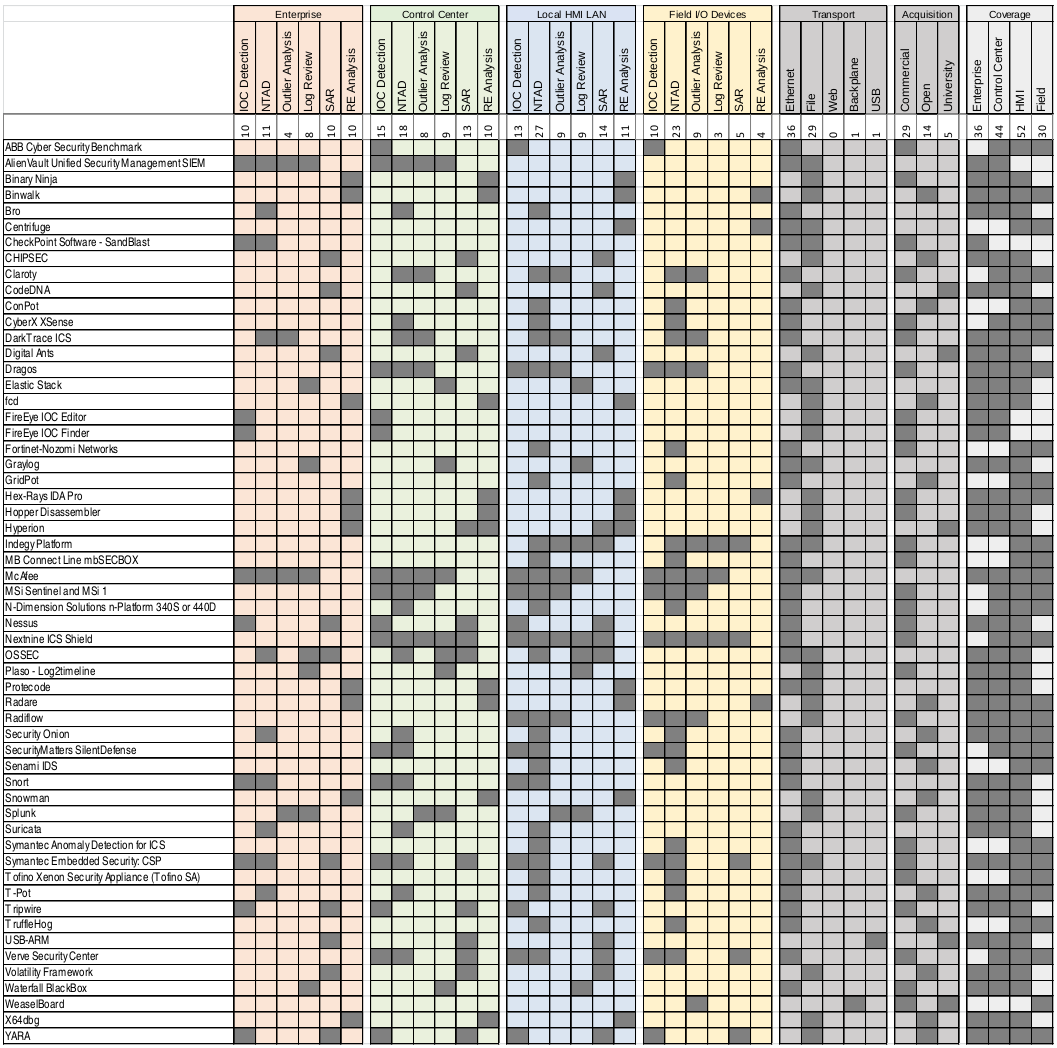
\includegraphics[width=\textwidth]{figuras/comparison_ics.png}
	\caption{Comparison by attributes of the most important ICSs\cite{comparison_ics}}
\end{figure}

\linej
\linej
One of the problems of a comparison in a table like this is that it fails to show how much a tool excels or lacks in the features it shares with others, how easy it is to use and other factors that can decide the right tool. The most relevant alternative technologies to OSSEC for this project are\cite{comparison_tools}:
\begin{itemize}
	\item Sagan: An open source HIDS, but only supports *nix operating systems (Linux, FreeBSD, OpenBSD, etc) and it lacks in features compared to OSSEC.
	\item YARA: Is not an IDS or IPS, it is just a tool that does pattern/string/signature matching, but it excels at it in performance, results and easiness to write the rules. It can be used to scan the \textbf{memory} for known patterns. YARA is being used widely in cybersecurity, for example by Avast, Kaspersky Lab, VirusTotal and McAfee Advanced Threat Defense\cite{who_is_using_yara}. We could build a system to use YARA to scan files but always combined with at least another tool, but we prefer to stick to a tested IDS.
\end{itemize}
\linej
Due to their popularity is worth mentioning the next tools, even though they are only for network:
\begin{itemize}
	\item Bro: Is an open source IDS and supports only Linux, FreeBSD, and Mac OS.
	\item Snort: Is the most popular open source IDS/IPS, but can be expensive in processing power.
	\item Suricata: Another open source IDS/IPS solution. It provides hardware acceleration and multi-threading to improve the scanning speed.
\end{itemize}
\linej
Most of the attributes in the previous comparison do not matter to us.
We chose OSSEC because the problems found on the alternatives.
Also OSSEC offers a reliable way to use an already done and thoroughly tested IDS, which we can enhance to our needs without much work.
To even ease more this we will use Wazuh, a fork of OSSEC.

\section{Objectives}
Quality is valued more than quantity in this project. Therefore anything will be reworked or discarded if it does not fully satisfy the student, Tarlogic or the professor.
\linej
\linej
The main objective is to improve intrusion detection in IDS. This can be accomplished in several ways:
\begin{itemize}
	\item Adding or changing functionality of an already existing technology.
		\subitem Coding on core or additions.
		\subitem Configuration or input of the program.
\end{itemize}
\linej
In this project the focus is on the configuration, particularly of rules to detect certain attacks. Is necessary to fully understand the attacks first to code its detection, therefore they also will need a fair amount of time.
It is important to explain the attacks and their detection clearly, in order to make this work useful for anyone else and ease any changes.
\linej
\linej
We will use OSSEC through Wazuh to code rules and decoders, without the need to change any code of the program itself.
This means this project can focus directly on detection without the need to create a full system from scratch.
If it were to be convenient to modify the detection system itself it would be considered, depending on the importance, the progress and the remaining time of the project.
\linej
\linej
The rest of the objectives can be met with each of the increments, that may or may not be done in this project (depending on the progress).
Because this project does not have a set of must have objectives they were planned in a modular fashion. Still some of them were marked as essential and if they were not to be met it would mean the failure of the project. More on its section on page \pageref{increments}.

\section{Structure of this document}
%TODO
This document has TODO chapters:
\begin{itemize}
	\item In \textbf{chapter 1} 
	\item In \textbf{chapter 2} 
	\item In \textbf{chapter 3} 
	\item In \textbf{chapter 4} 
	\item In \textbf{chapter 5} 
	\item In \textbf{chapter 6} 
	\item In \textbf{chapter 7} 
\end{itemize}



\cleardoublepage
\chapter{Requirements}

%Especificación de requisitos: debe indicarse, polo miúdo, a especificación do 
%Sistema, xunto coa información que este debe almacenar e as interfaces con outros 
%Sistemas, sexan hardware ou software, e outros requisitos (rendemento, seguridade, 
%etc).


The requirement specification is a full description of the software the project is to develop.
\linej
PMBOK\cite{pmbok} states that requirements are conditions or capabilities that a product must meet to satisfy the contract.
The requirements expose the needs of the client, which have to be accomplished to finish the project successfully.
In this project the requirements will be fullfilled in multiple stages along the project.
\linej
Note that the client in this case is Tarlogic even if the product is a contribution to an open source project.

\linej
\linej
This specification contains:
\begin{itemize}
	\item \textbf{Use cases}: Functionalities that the software will provide.
	\item \textbf{Requirements}: Depending of their type they can describe features, data, relations, properties or any details necessary to explain the system without ambiguity, in a way it can be easily understood.
\end{itemize}

In this project the functional requirements are not included because they can be considered a redundant version of the use cases, because both describe the same functionalities.
Uses cases were chosen over functional requirements because they were considered to be easier to understand and have greater detail. If this project had the need of a very complex requirement specification it would be interesting to have both, as each could help to understand the other better, but in this project the specification should be quite simple.






\section{Use cases}
A use case is a description of all the ways an end-user wants to ``use'' a system. These ``uses'' are like requests of the system, and use cases describe what that system does in response to such requests. In other words, use cases describe the conversation between a system and its user(s), known as actors. Although the system is usually automated (such as an Order system), use cases also apply to equipment, devices, or business processes.\cite{use_case_definition}


\subsection{Use cases actors}
The actors are entities external to the system that interact with it. They can be other systems, persons or even time.

%\subsection{Use cases description}
\subsection{Use cases list}

\section{Requirements analysis}

\subsection{Non functional requirements}

\subsection{Functional requirements}
As mentioned before these are omited because of the redundancy with use cases.

\subsection{Domain requirements}


\cleardoublepage
\chapter{Technologies and tools}
%TODO

\section{Introduction}
Wazuh is a fork of OSSEC. It adds a RESTFul API, has a more updated ruleset and is easier to install (providing ELK over OSSEC).
\begin{figure}[H]
  \centering
	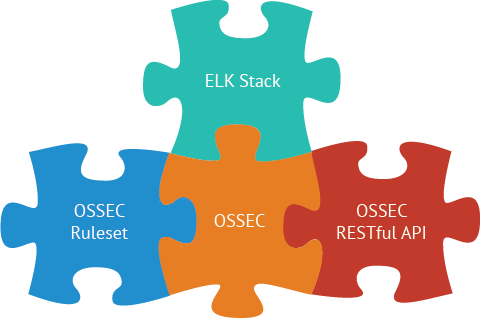
\includegraphics[width=.6\textwidth]{figuras/wazuh_stack.png}
	\caption{The different parts of Wazuh\cite{wazuh_stack}}
\end{figure}
\linej
The most interesting qualities of Wazuh for this project are\cite{wazuh_index}\cite{wazuh_documentation}: %necessary redundancy
\begin{itemize}
	\item \textbf{Rootkits detection}: Rootkits are commonly used after an attack has suceeded to use the computer of the victim leaving no traces.
	\item \textbf{File integrity monitoring}: It can provide detection of intrusions by identifying changes in content, permissions, ownership, and attributes on the monitored files. It can be used to comply with GDPR (General Data Protection Regulation).
	\item \textbf{Scalability and multi-platform}: This means that the work on this project could really be used in real work environments.
	\item \textbf{Configuration management}: The configuration is managed by the Wazuh server (Wazuh manager) and the agents can be grouped, allowing custom, grupal or global gathering and detection for each agent.
	\item \textbf{Multiple sources of data}: The scanned data can be from logs, output of commands or databases. %TODO more?
	\item \textbf{Active response}: Automated remediation to security violations and threats, to mitigate more the possible damage. For example to stop the Internet connection to isolate a compromised system.
	\item \textbf{Improved ruleset}: It is the combination of rules and decoders. Having this ruleset out of the box reduces the workload of this project. It can also serve as reference and complement some of the rules and decoders that this project intends to work on.
	\item \textbf{Open source, free and easy to contribute to}: This is optional but nice, as it offers a chance to an unexperienced student to contribute in a real and useful project. The project is hosted on Github and Google Groups. In this project the contribution would be to the ruleset\cite{wazuh_ruleset} and not to the core of Wazuh\cite{wazuh} or the documentation\cite{wazuh_documentation2}.
\end{itemize}
\linej
The RESTFul API interacts using OSSEC commands and would be interesting if this project were related to a tool issuing queries to Wazuh, but this is not the case. Anyway it is still something valuable to have as these kind of tools are very common nowadays.

\linej
\linej
Wazuh provides support and integration with multiple important tools and technologies:
\begin{itemize}
	\item Docker container for OSSEC: An ossec-server image with the ability to separate the ossec configuration/data from the container.
	\item Puppet and Ansible: For massive deployment. This can be very helpful to setup a big environment mostly because even being no need to put configuration files in the agents for Wazuh often is necessary to configure other things and the process of registering agents can be tedious manually.
	\item Network IDS integration: Gives the option to use OwlH and integrate Suricata and Bro to generate alerts in Wazuh.
	%\item Splunk infrastructure: Comprised of a Splunk Enterprise instance as indexer and a Splunk Forwarder node, as well as the Wazuh app for Splunk.
	\item VirusTotal: A free virus, malware and URL online scanning service that combines more than 40 antivirus solutions.
	\item OSQuery: Osquery can be used to expose an operating system as a high-performance relational database. This allows you to write SQL-based queries to explore operating system data.
\end{itemize}
\linej
The use of these depends on the scenario, but we only take interest in VirusTotal and Network integration. They can work as secondary detection methods for the most critical or complicated cases.

\section{Wazuh architecture}

A basic Wazuh setup has the next components\cite{wazuh_architecture}:
\begin{itemize}
	\item Wazuh server: Runs the Wazuh manager, API and Filebeat (Filebeat is only necessary in distributed architecture). It collects and analyzes data from deployed agents.
	\item ELK stack: It reads, parses, indexes, and stores alert data generated by the Wazuh server. The ELK stack is flexible, highly configurable and very used in big data.
	\item Wazuh agent: Runs on the monitored host, collecting system log and configuration data and detecting intrusions and anomalies. It talks with the Wazuh server to which it forwards collected data for further analysis.
\end{itemize}
\linej
The main difference with the architecture of OSSEC is the ELK stack, because OSSEC leaves the choice of tools to the user. ELK stands for the combination of:
\begin{itemize}
	\item Elasticsearch: Gets the data and allows search queries and analysis.
	\item Logstash: Transforms the data to the desired format. This step can make alike data from different log and output formats, trivializing the decoders work.
	\item Kibana: Shows the data in a web browser, with graphs and options like grouping and time interval. This is often easier than to write commands to scan the OSSEC log in the Wazuh server, as the data of interest tends to stay the same.
\end{itemize}
\linej
There are two possible architectures for this setup: having the ELK stack in the same machine that the Wazuh server (singlehost) or in a separated one (distributed). Each has advantages and disadvantages and in this project we will use the singlehost because in our case there are no constraints and is easier to set up and is more efficient.
\begin{figure}[H]
  \centering
	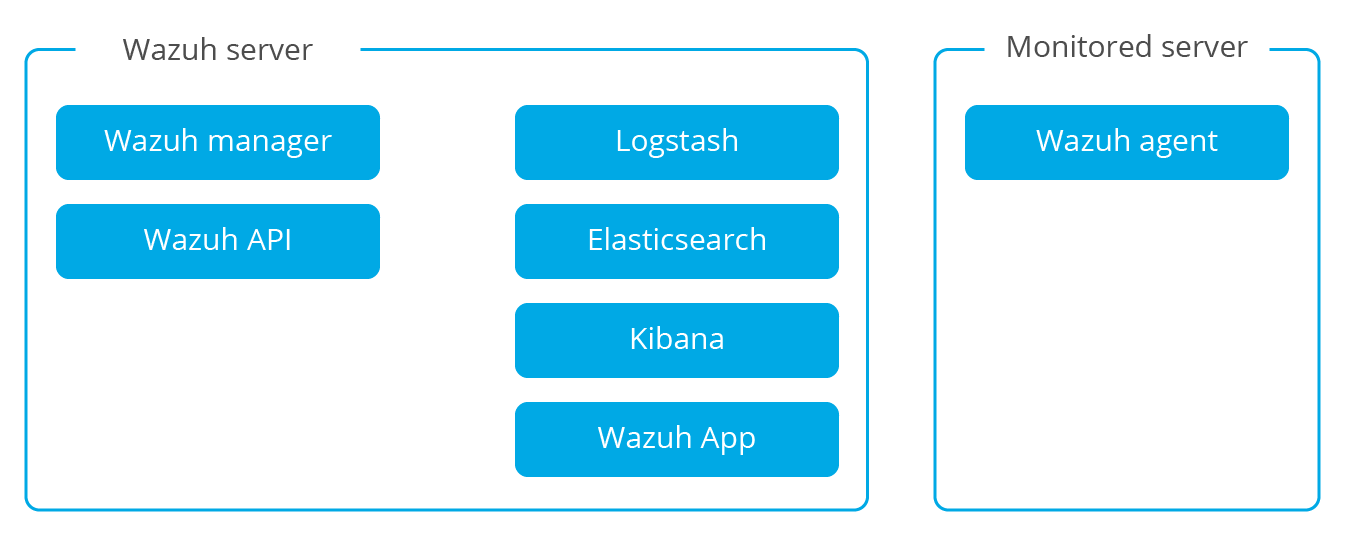
\includegraphics[width=\textwidth]{figuras/wazuh_singlehost.png}
	\caption{Singlehost architecture}
\end{figure}

\begin{figure}[H]
  \centering
	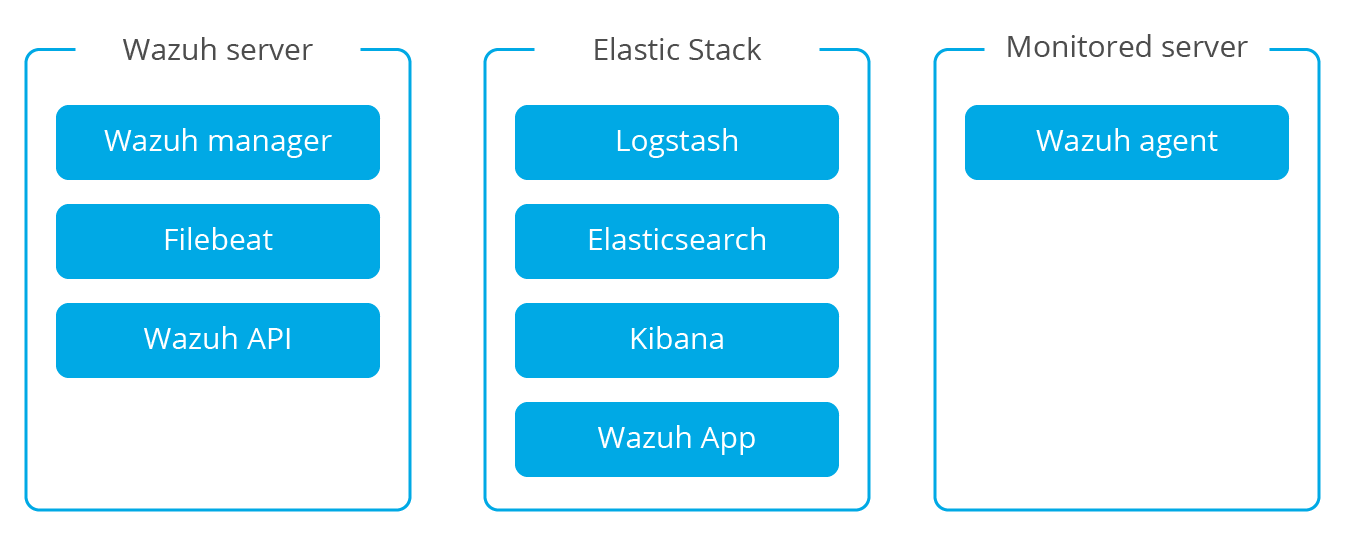
\includegraphics[width=\textwidth]{figuras/wazuh_distributed.png}
	\caption{Distributed architecture}
\end{figure}
\linej
To understand better the communications and data flow in Wazuh we will now get into more detail on the process\cite{wazuh_architecture2}\cite{wazuh_data_flow}.
\linej
\linej
Wazuh agents use the OSSEC message protocol to send collected events to the Wazuh server over port 1514 (UDP or TCP). The Wazuh server then decodes and rule-checks the received events with the analysis engine. Events that trip a rule are augmented with alert data such as rule id and rule name. The Wazuh message protocol uses a 192-bit Blowfish encryption with a full 16-round implementation, or AES encryption with 128 bits per block and 256-bit keys.
\linej
Logstash formats the incoming data and optionally enriches it with GeoIP information before sending it to Elasticsearch (port 9200/TCP). Once the data is indexed into Elasticsearch, Kibana (port 5601/TCP) is used to mine and visualize the information.
\linej
The Wazuh App runs inside Kibana constantly querying the RESTful API (port 55000/TCP on the Wazuh manager) in order to display configuration and status related information of the server and agents, as well to restart agents when desired. This communication is encrypted with TLS and authenticated with username and password.

\begin{figure}[H]
  \centering
	\makebox[\textwidth][c]{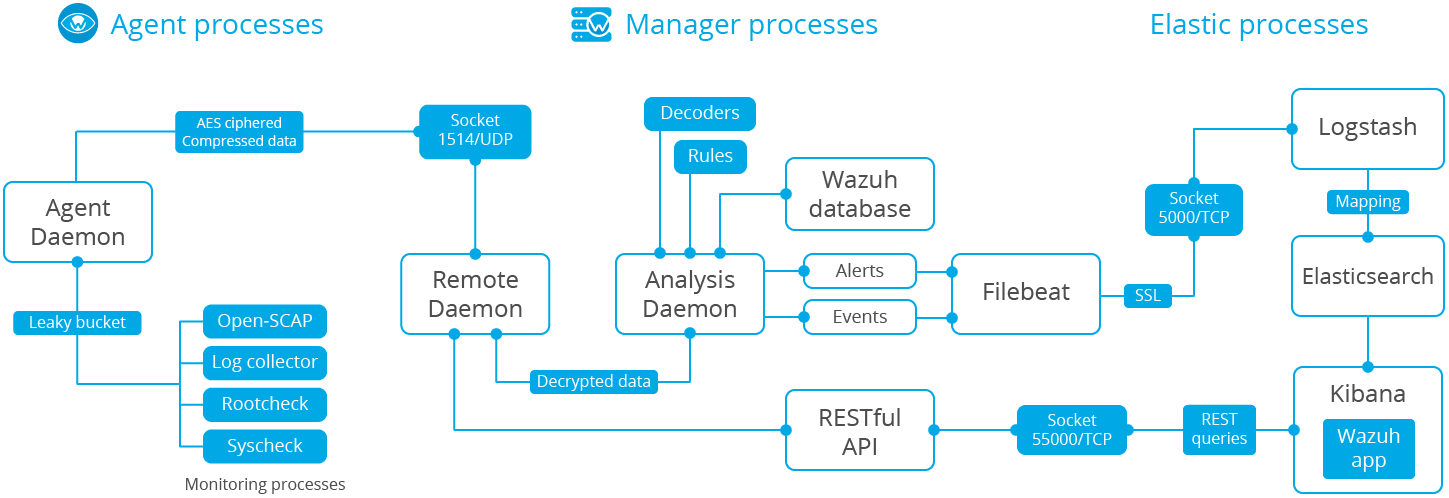
\includegraphics[width=1.2\textwidth]{figuras/wazuh_data_flow1.png}}
	\caption{Communications and data flow}
\end{figure}
\linej
Both alerts and non-alert events are stored in files on the Wazuh server in addition to being sent to Elasticsearch. These files can be written in JSON format and/or in plain text format (.log, with no decoded fields but more compact). These files are daily compressed and signed using MD5 and SHA1 checksums.


\section{Rules and decoders}
They constitute the main part of this project and they can be used to detect application or system errors, misconfigurations, attempted and/or successful malicious activities, policy violations and a variety of other security and operational issues\cite{wazuh_index}. Wazuh is quite helpful with the features and documentation of the ruleset and in this project the already existing rules and decoders were a great help as examples.
\linej
\linej
Rules can be added in \textit{/var/ossec/etc/rules/} and decoders in \textit{/var/ossec/etc/decoders/} without any issue, but to change the already existing ones in \textit{/var/ossec/ruleset/rules/} or \textit{/var/ossec/ruleset/decoders/} is a bad idea because the next changes in those files from updates would overwrite them.
%The solution is to copy the code (actually only the id is needed) of the existing item to the folder where we can add new ones, make the desired changes add \textit{overwrite=``yes''}\cite{wazuh_custom}.
\linej
\linej
As mentioned before Wazuh adds its own ruleset over the one provided by the OSSEC project. The next table shows about 20\% of the combined ruleset that Wazuh uses, where ``Out of the box'' means that the source was the OSSEC project.
\begin{figure}[H]
  \centering
	\makebox[\textwidth][c]{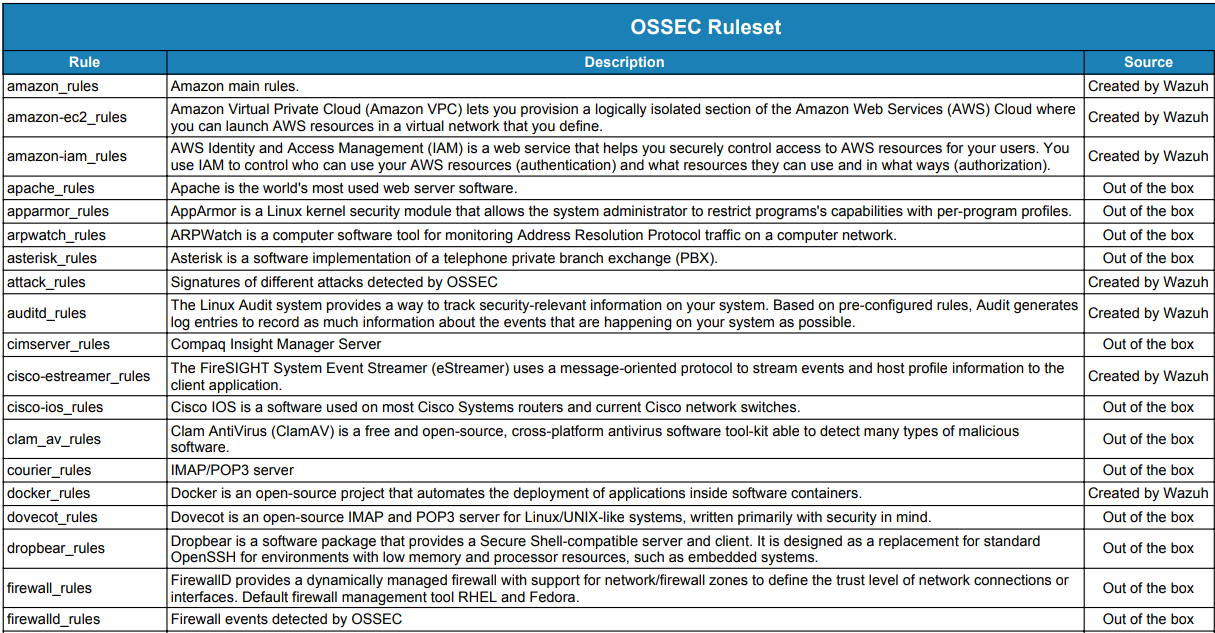
\includegraphics[width=1.1\textwidth]{figuras/wazuh_ruleset.png}}
	\caption{Portion of the ruleset used by Wazuh\cite{wazuh_ossec_ruleset}}
\end{figure}
\linej
Wazuh provides a way to manually test how an event is decoded and if an alert is generated with the tool \textit{/var/ossec/bin/ossec-logtest}\cite{wazuh_testing}, which is very useful for debugging.
To use it you only need to introduce the data as it would be received by the Wazuh manager.
Is possible to show which rules are tried and which trigger an alert for each event.
This tools does not need a restart of the wazuh-manager service whenever changes want to be tested because it reads the configuration directly.
\linej
But is also worth to mention that some times it can be missleading because it does not work in the same way as the manager.
For example the logtest may show that the log matches a certain rule but actually it has matched a previous one silently.
\linej
\linej
For example for this input:
\linej

\includegraphics[width=\textwidth]{figuras/ossec-logtest_input.png}
\linej
We get the next output:
\begin{figure}[H]
  \centering
	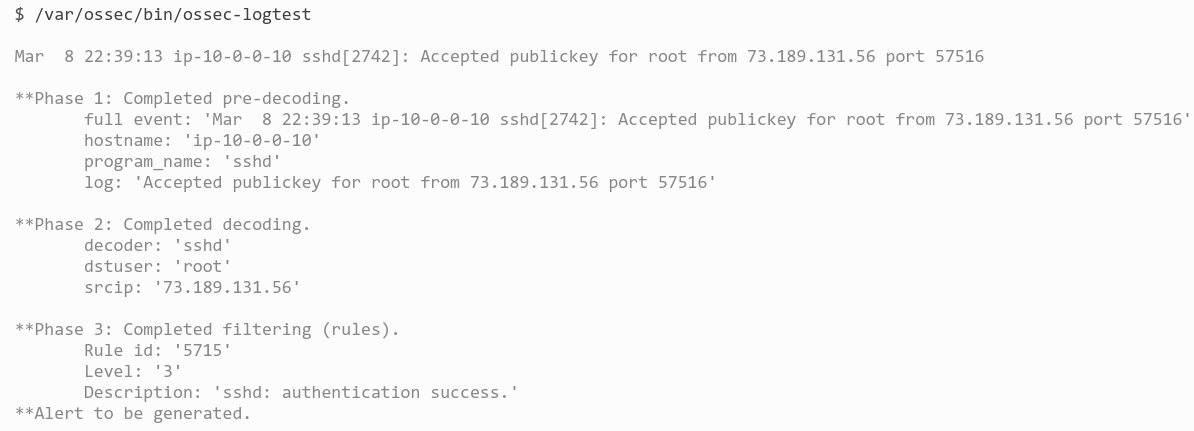
\includegraphics[width=\textwidth]{figuras/ossec-logtest_output.png}
	\caption{Example of output for ossec-logtest}
\end{figure}
\linej
%TODO cambiar currently in version
After version 3.0.0 (we are currently in 3.9) Wazuh incorporates an integrated decoder for JSON logs enabling the extraction of data from any source in this format. This can be very useful in many situations, for example trivializing the generation of alerts for Suricata (without the need for a decoder just for Suricata)\cite{wazuh_json}.
\linej
\linej
Another interesting feature is to check if a field extracted during the decoding phase is in a CDB list (constant database). The main use case of this feature is to create a white/black list of users, IPs or domain names.\cite{wazuh_cdb}.

Usually this chapter would be ``Design and Implementation'', but it was not needed because there was no serious software development during this project, as explained before.
Still a description of the components and their communication in the system is needed to fully understand it.
\linej
\linej
This project was run under a GNU/Linux distribution in one of the personal computers of the student.
Said computer has 20GB of RAM, an \textit{i5-2500k} processor and about 500GB of free disk storage for this project.
\linej
\linej
Hosting services were considered but discarded, because their biggest advantage would be to be able to work on this project anywhere (since the only user is the student). This is something that can be achieved in a home computer with port redirection and either knowing the external ip of the router or using a naming service. There was no need to connect from the outside because the student had no more classes after december. When outside, time was better spent on research or on this document.

\section{Virtual machines}
VirtualBox was chosen as the host program of the virtual machines because it was the one the student had the most experience with.
\linej
This laboratory consist of multiple virtual machines, that represent:
\begin{itemize}
	\item An enterprise domain of Windows computers, named \textbf{Wazuh.local}, managed by Windows' Active Directory:
		\begin{itemize}
			\item Windows Server 2019, as Domain Controller of the Active Directory.
			\item Windows Server 2019, as a file server.
			\item Windows 10, as a basic workstation.
		\end{itemize}
	\item The Wazuh server: A CentOS 7. As mentioned before\ref{singlehost}, we are using a single server to host both the Wazuh manager and the ELK stack.
	\item An offensive security box: In this case with Kali Linux. This is used to access the Windows boxes in some of the attacks.
\end{itemize}

\begin{figure}[H]
  \centering
	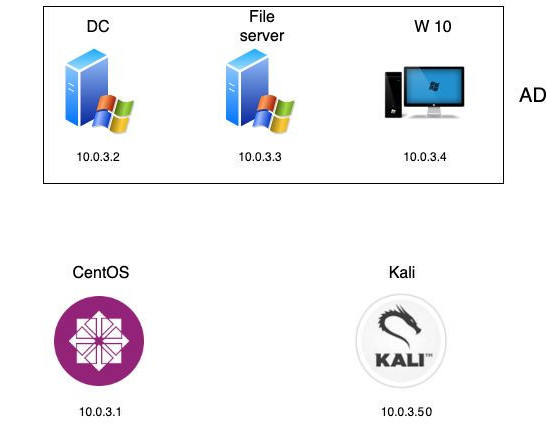
\includegraphics[width=\textwidth]{figuras/virtual_machines.jpg}
	\caption{Virtual machines in the project}
\end{figure}
\linej
Every machine has two network interfaces, one for the internal network (10.0.3.0) and another for accessing the internet connection of the host.
Each of the Windows boxes have a Wazuh agent installed, that reports to their manager (server) in the CentOS box.
All the ruleset changes and log processing was done directly on the CentOS machine.
\linej
\linej
Most of the time only the DC and the CentOS machine were powered on, but when all of them were being used at the same time they consumed about 12GB of RAM. Leavin aside booting, they did not affect performance in a perceptible way, either one to each other or to the host.
\linej
\linej
Snapshots were taken when significant changes were made, like relevant installation or configuration. Then the virtual machines with their snapshots were copied to a couple of external disks as backup. At the end of the project near 60 snapshots were taken and the virtual machines with their snapshots were using about 160GB of disk space.



\section{Technologies and tools in detail}
This section recopilates the main software used in the project for an easier overview.

\subsection{For development and configuration}
\begin{itemize}
	\item Wazuh: Wazuh\cite{wazuh} is the core of this project and some of the configuration of the system had to be done with it. In this project ruleset files were created to detect the targeted threats.
	\item Sysmon: Sysmon\cite{sysmon} reports events based on its configuration, which in most cases give more insight of the status of the system than normal Windows events.
	\item PowerShell: Some basic scripting\cite{memoria_github} was done in PowerShell to mimic attacks and to perform a particular detection with a remote command.
\end{itemize}

\subsection{For pentesting}
\begin{itemize}
	\item PowerShell scripts: Third-party tools written in PowerShell were used to mimic attacks.
	\item PowerShell and Windows builtins: Some harmless PowerShell commands were used in combination with Windows builtins in order to extract useful data for an attacker.
	\item Linux shell programs in GNU/Linux: They were used in order to fully understand how some of the security was implemented in the Windows systems. For example their network share was first tested with the Samba command \textit{smbclient}.
	\item Metasploit: It was used as framework\cite{metasploit} for getting information and to exploit security vulnerabilities, mimicking an attacker.
	\item Mimikatz: Mimikatz\cite{mimikatz_github} was one of the most used tools for extracting data and gaining privileges.
	\item Other third-party tools were used to dump data from memory or extract credentials. They were only used in order to gather enough data to assure the identification of attack patterns from different sources.
	\item OpenSSL\cite{openssl}: Set of tools for secure communications. In this project it was used to encrypt files for crypto ransomware testing.
	\item Trid\cite{trid}: It is a tool for scanning files in order to find their type.
	\item Dharma\cite{dharma}: It is a crypto ransomware malware that was executed in order to test the configuration against a real software.
\end{itemize}

\subsection{For processing logs}
\begin{itemize}
	\item The Kibana plugin for Wazuh: It provides an easy and fashionable way to show the triggered alerts with a web browser. It was only used at first, before it felt too slow and shallow.
	\item Linux shell programs in GNU/Linux: The most used were Grep, AWK and Tmux. They were used to process the logs of Wazuh for most of the project. These logs include the received events and the triggered alerts. They were a good fit because they are easy to write commands on, they are fast and the queries needed for this project were quite simple. Grep was used for finding events with certain patterns. AWK to parse logs for easier comprehension. Tmux is a terminal multiplexer, which is basically a program that controls a bunch of terminals, and was used to manage the shells and to find and copy strings in them, similar to an Integrated Development Environment (IDE).
	\item The Windows Event Viewer: To troubleshoot inspecting the logs generated from Sysmon. Some times under heavy load (particularly after booting) the agent could not send the data to the manager without a significant delay of a couple of minutes.
\end{itemize}

\subsection{For the documentation}
\begin{itemize}
	\item Git: It was used to store the memory and manage its changes, through a Github repository\cite{memoria_github}.
	\item Vim + \LaTeX + Latexmk: Vim was used as the text editor to write all the documentation and most of the ruleset and scripts. This was easier for me than using other editors because I have a fair amount of customization for Vim, in my general purpose dotfiles\cite{andresgomezvidal_gitlab}. \LaTeX was the medium the memory was writen in (including the WBS and Gantt diagrams), with Latexmk for its compilation.
	\item Draw.io: A web application for general purpose drawing\cite{drawio}. It was used for making diagrams in this project.
	\item Simplescreenrecorder: It is a GNU/Linux program. It was used to record videos during critical tasks using the virtual machines. These serve just as a way to assure the student these tasks were done exactly as he remembers them, or how to reproduce them.
	They did not take much disk space (about $\sim$110MB per hour) while still having decent image quality. The recording settings were 15 frames per second and h264 codec with a constant rate factor of 32.
	\item Linux shell programs: Some simple commands to make sure no minor elements are forgotten. For example that all references and images are used, and that any relevant acronyms are explained in the glossary.
	\item Aspell: It is a spell checker\cite{aspell}, this is a program for reviewing that words are writen correctly in the specified language. This program has a mode for \LaTeX that ignores its commands without the need of a special dictionary.
\end{itemize}



\cleardoublepage
\chapter{Project management}
A project is temporary in that it has a defined beginning and end in time, and therefore defined scope and resources.
And a project is unique in that it is not a routine operation, but a specific set of operations designed to accomplish a singular goal.
\linej
Project management, is the application of knowledge, skills, tools, and techniques to project activities to meet the project requirements\cite{pmi_project_management}.
It is important to note that the actions on each area of the project may affect other areas, increasing the difficulty of the management.

\section{Scope management}
The management of the scope of the project has the necessary processes to guarantee that the objectives are met.
The scope management allows the project to start focused in what really matters, not losing time in irrelevant details or desirable additions that we can not implementent, by identifying and describing the necessary tasks.

\subsection{Description of the scope}
This project tries to improve the detection of intrusions with the already existing HIDS Wazuh. This kind of objective can be accomplished by very different approaches. This is because the software can be used in many scenarios, is very related to other software and is in active development.
\linej
Even though some increments can be considered difficult due to the amount of new technologies and tools there should be no problem to meet the basic objectives.
This is because we have the \textbf{freedom to adapt the scope at any time} and there is more than enough time for the essential parts of the project.
\linej
\linej
From before the start of the project the interest was not on producing something specifically, but in what we could produce after having some research. This uncertainty has been reduced with planning and research for the pre-project documentation, but is still something to take in mind in the management of the project.
\linej
In practice it means that we do not expect all the planning to work and are ready to make adjustements at any time.

\subsection{Acceptation criteria}
In order to the product to be accepted the essential requeriments need to have been accomplished before the time limit of the project.
The rest of the requirements will be implemented if there is enough time left.

\subsection{Increments} \label{increments}
The essential increments to the project are:
\begin{itemize}
	\item Increment 1: \IncrementoUno.
	\item Increment 2: \IncrementoDos \ that are not builtin in a standard system installation, like Sysmon. By itself having more data does not mean more attack detection, but certain attacks could not be identified without them.
	\item Increment 3: \IncrementoTres.
\end{itemize}
\linej
These were chosen because they seem the most straightforward and Wazuh needs tangible security measures against common threats. From the assumed viewpoint these seems to be were Wazuh lacks the most right now.
\linej
\linej
The rest of the increments are considered optional and can be removed if there is not enough time left. The order is based on the estimation of the relevance of the increment for Wazuh and our project. This means for example having in mind the time estimation for the increment without stretching.
\begin{itemize}
	\item Increment 4: \IncrementoCuatro. This is considered a very important increment because it could be a selling point for some enterprises, that probably do not want the same level of security for all their computers and the time to set it up (or at least from scratch). There is a chance that something like this already exists and can be used instead of manually writing configuration profiles and scripts. For example Wazuh supports integration with OpenScap, an open source security compliance to manage configuration and tools. In any case the investigation at the start of the increment should find it.
	\item Increment 5: \IncrementoCinco. Tarlogic stated that they would like to have this increment specifically.
	\item Increment 6: \IncrementoSeis. This could have more or less the same impact as increment 1 for some clients, but Tarlogic was more interested in Windows and Wazuh seems to be more oriented towards GNU/Linux.
	\item Increment 7: \IncrementoSiete. The problem of this increment is that VirusTotal's public API key has more limited features and has a 4 requests/minute limitation\cite{virustotal_faq}. We asume the use of a public API key because it would fit the profile of a client using Wazuh, which has no charge. Also the exploration on this increment could not really be considered more than a patch to Wazuh, without really improving it, but still it would be an effective workaround for the problems we can not solve right now with only Wazuh.
\end{itemize}

\subsection{Products of the project}
At the end of the project the next elements will be delivered:
%TODO Products of the project
\begin{itemize}
	\item 
	\item 
	\item 
\end{itemize}

\subsection{Exclusions} \label{exclusions} 	%necessary redundancy with introduction?
As in any project of this kind we had to leave some ideas behind.
For example an interesting way to to take advantage from IDS is to set up a honeypot (a false server just to be compromised) and learn from the intrusions suffered, improving the defenses (firewall, IPS and IDS) for the real servers.
\linej
There are some honeypot implementations that automate (for example with machine learning) the generation of rules for certain IDSs, but is not yet a trend because there are problems\cite{snort_learning}\cite{honeypot_weka_learning}\cite{honeypot_ossec_trees}\cite{snort_honeypot}:
\begin{itemize}
	\item Experienced attackers have learned to avoid honeypots, because they are easy to identify due to the low security they have.
	\item It is not trivial to automate correctly the defense based on the information of the system, because its state can be very complex (for example due to more than one attack at the same time).
\end{itemize}
\linej
This automation would be a great solution to the need to update manually the rules and depending of the case it could even protect against day-zero vulnerabilities. Despite being interesting this was not even included as a possible increment because the complexity of the task.
If this were to be included probably it would have not ended well, because is something that even experts in cybersecurity have some trouble with at the moment.
\linej
There is also the option to use honeypots only to detect attackers with the existing rules, without looking for improving them. Normally they are easy to set up, for example clonning the virtual machine of a server and making it easier to access, removing critical data and monitoring some kind of bait for the attacker. They are not excluding from this project, but they are not explicity set to be in an increment; they will be used if they turn to be useful in some regard.
\linej
\linej
There is always a risk of intrusion disabling the security of the system.
This is more or less the same problem that cybersecurity has in any scenario and there is no way to guarantee that it will not happen.
In this case the attacker would have to somehow not be detected or cut the IDS before it sends the alert but in a way that is not suspicious (for example shutting it down completely would be obvious for a central manager).
Researching a bit on these malicius techniques is not out of the question, as they are a common occurrence after attacks, but probably there will not be enough time.
\linej
Our approach is to trust the IDS and work on improving the detection of known attacks instead of the worst case scenario.
If there was enough time we could have considered finding a solution for this problem.
\linej
\linej
Exploring a HIDS with behaviour analysis was also considered but rejected because it is more fit for a network approach. Still is a shame there is no enough time to explore IDS based on behavior analysis, because their protection against much zero-day attacks.
\linej
\linej
We focus on a host approach, leaving aside most of the detection capabilities for the network. This means less detection, a lower detection rate, less options to improve the detection process and later and worse performance in the analysis of network traffic. Having chosen to focus on HIDS the best way to have also a good NIDS process would be the use of a NIDS along with our HIDS.
\linej
Wazuh offers this kind of integration with Bro and Suricata and probably it would be possible to extend it to other NIDSs like Snort, but yet again we had to choose and this was not a priority at the moment.
\linej
\linej
For Windows systems monitoring registry changes could be explored in the same way we study events in this project.
Wazuh can detect changes in the registry as it does with other files: registering its hashes and checking for changes periodically.
Windows has audit options for registry, which generate events that allow to monitor it with Wazuh.
Sysmon also has events for the registry changes: creation, deletion, renaming and value modification.
Because the lack of time and experience this idea was left behind for most of the project, leaving aside a minor part in the last increment done.
\linej
\linej
YARA is very interesting for this kind of project, but it belongs to the Virustotal pack of malware detection tools and so it could be used with Wazuh with a Virustotal API key. The free version only allows a few queries and the option of getting a premium key was not considered. There has been for months an open issue in the Github page of Wazuh for integrating it with YARA (as other IDSs have done before), which has recently evolved to an issue to integrate YARA into Wazuh as a module\cite{yara_module}.
Unfortunately this was not done before the first increment of the project was completed, so there was no chance to use it in the end.
\linej
\linej
Sigma\cite{sigma} is a project that mantains a Generic Signature Format for SIEM Systems. This means a set of files describing threats and relevant information about them, like signatures and false positives. An automated integration with Sigma would also be possible with a script to convert Sigma rules to OSSEC, which was not even considered because it falls out the scope. It could be been used in some parts of this project as a manual resource to find patterns to look for, but in the end was not necessary.
\linej
\linej
Another idea that was left behind was to ensure the protection of the Wazuh agent itself in case of attack. This would cover the detection of processes attempting to stop or or modify the agent program or the data sent to the manager. This can also be applied to other actions like disabling logs and modifying settings or security policies. It is interesting for the project because it would be one of the first and most effective steps that a smart attacker would do to avoid being detected.

\subsection{Restrictions}
Leaving aside the time constraint of \projecthours \ hours, the two main factors to decide what improvements to choose for this project are a student without experience in proffesional cybersecurity and that we want some kind of inmediate results from this project.
This is why instead of a pure research project (for example machine learning with IDS), we opted for a more traditional and safer approach.
Because of this most of the increments were optional (due to the high probability of initial scope being too ambitious), but the first increments are considered vital to the project.
\linej
\linej
A minor restriction is to deliver correctly all the products of the project before the presentation date.


\section{Risk management}

\subsection{Risk metrics}

\begin{table}[H]
	\centering
	\begin{tabular}{|l|l|}
		\hline
		\rowcolor{gray!30}
		Chances of the risk happening & Probability \\ \hline
		$\geq$80\% & \cellcolor{red!60}High\\ \hline
		Between 30\% and 80\% & \cellcolor{yellow!40}Medium\\ \hline
		$\leq$30\% & \cellcolor{green!60}Low\\ \hline
	\end{tabular}
	\caption{Probability classification of risks}
\end{table}


\begin{table}[H]
	\centering
	\begin{tabular}{|l|l|}
		\hline
		\rowcolor{gray!30}
		Resource in Place / Effort / Cost & Impact \\ \hline
		$\geq$20\% & \cellcolor{red!60}High\\ \hline
		Between 10\% and 20\% & \cellcolor{yellow!40}Medium\\ \hline
		$\leq$10\% & \cellcolor{green!60}Low\\ \hline
	\end{tabular}
	\caption{Impact classification of risks}
\end{table}


\begin{table}[H]
	\centering
	\begin{tabular}{|c|c|c|c|c|}
	\hline
		\multicolumn{2}{|c|}{\multirow{2}{*}{\large\textbf{Exposition}}} & \multicolumn{3}{c|}{Probability}\\
		\multicolumn{2}{|c|}{} & \cellcolor{gray!15}\textbf{High} & \cellcolor{gray!15}\textbf{Medium} & \cellcolor{gray!15}\textbf{Low}\\ \hline %\cline{3-5}
		\multirow{3}{*}{Impact} & \cellcolor{gray!15}\textbf{High} & \cellcolor{red!60}High & \cellcolor{red!60}High & \cellcolor{yellow!40}Medium\\
		& \cellcolor{gray!15}\textbf{Medium} & \cellcolor{red!60}High & \cellcolor{yellow!40}Medium & \cellcolor{green!60}Low\\
		& \cellcolor{gray!15}\textbf{Low} & \cellcolor{yellow!40}Medium & \cellcolor{green!60}Low & \cellcolor{green!60}Low\\ \hline
	\end{tabular}
	\caption{Method of calculation of Exposition based of Probability and Impact}
\end{table}

\subsection{Risk types}

\subsection{Risk identification}


\newcommand{\Runo}{Optimist planning, ``best case'' (instead of a realistic ``expected case'')}
\newcommand{\Rdos}{Bad requirement specification}
\newcommand{\Rtres}{Design errors}
\newcommand{\Rcuatro}{Lack of key information from sources}
\newcommand{\Rcinco}{Lack of feedback or support from the security consultants of Tarlogic}
\newcommand{\Rseis}{The learning curve of some technologies is larger than expected}
\newcommand{\Rsiete}{The unexplained parts of the project take more time than expected}
\newcommand{\Rocho}{Can not access source material}
\newcommand{\Rnueve}{Unexpected changes to any of the software used in the project}
\newcommand{\Rdiez}{Loss of work}
\newcommand{\Ronce}{Wrong management of the project's configuration}
\newcommand{\Rdoce}{A delay in one task leads to cascading delays in the dependent tasks}
\newcommand{\Rtrece}{The student can not find a way to detect a certain occurrence}
\newcommand{\Rcatorce}{The quality of the product is not enough}
\newcommand{\Rquince}{Sickness or overwork}
\newcommand{\Rdieciseis}{Performance issues}
\newcommand{\Rdiecisiete}{Unnecessary work}
\newcommand{\Rdieciocho}{Optional requirements increment the time need to complet the project}


\begin{table}[H]
	\caption{Project risks}
	\begin{tabularx}{\textwidth}{|l|X|}
		\hline
		\rowcolor{gray!30}
		Identifier & Name \\ \hline
		%R-00 & The scope specified is too big\\ \hline
		R-01 & \Runo \\ \hline
		R-02 & \Rdos \\ \hline
		R-03 & \Rtres \\ \hline
		R-04 & \Rcuatro \\ \hline
		R-05 & \Rcinco \\ \hline
		R-06 & \Rseis \\ \hline
		R-07 & \Rsiete \\ \hline
		R-08 & \Rocho \\ \hline
		R-09 & \Rnueve \\ \hline
		R-10 & \Rdiez \\ \hline
		R-11 & \Ronce \\ \hline
		R-12 & \Rdoce \\ \hline
		R-13 & \Rtrece \\ \hline
		R-14 & \Rcatorce \\ \hline
		R-15 & \Rquince \\ \hline
		R-16 & \Rdieciseis \\ \hline
		R-17 & \Rdiecisiete \\ \hline
		R-18 & \Rdieciocho \\ \hline
	\end{tabularx}
\end{table}





\subsection{Risk analysis}


\begin{table}[H]
	\begin{tabularx}{\textwidth}{|l|X|}
		\hline
		\rowcolor{gray!30}
		Identifier & \textbf{R-001} \\ \hline
		Name & \Runo \\ \hline
		Description & An optimistic planning at the start of the project does not take into account problems or delays, and so it does not allocate time for them. \\ \hline
		Negative effects
			& Could mean the failure of the project if the objectives can not be accomplished in the time left. \\
			& Rework the planning. \\
			& Cascading delays.\\ \hline
		Probability & Medium\\ \hline
		Impact &  High\\ \hline
		Exposition &  High\\ \hline
	\end{tabularx}
\end{table}

\begin{table}[H]
	\begin{tabularx}{\textwidth}{|l|X|}
		\hline
		\rowcolor{gray!30}
		Identifier & \textbf{R-002} \\ \hline
		Name & \Rdos \\ \hline
		Description & The requirements specified at the beginning of the project are not specific enough, are not needed or there are new requirements after the beginning of the project. \\ \hline
		Negative effects
			& Need to redo the analysis of specifications. \\
			& Redo planning.  \\
			& Rework of related requirements and work based on them, including the need to test the results. \\
			& Possible failure of the project if the objectives can not be accomplished in the time left. \\ \hline
		Probability & High\\ \hline
		Impact &  High\\ \hline
		Exposition &  High\\ \hline
	\end{tabularx}
\end{table}

\begin{table}[H]
	\begin{tabularx}{\textwidth}{|l|X|}
		\hline
		\rowcolor{gray!30}
		Identifier & \textbf{R-003} \\ \hline
		Name & \Rtres \\ \hline
		Description
			& A design is not enough or is incorrect. \\
			& This can be found in later stages, when it is clear that the implementation based on the design would not satisfy the requirements. \\ \hline
		Negative effects
			& Having to redesign and maybe redo the work based on the design. \\
			& Minor delays. \\ \hline
		Probability & Low\\ \hline
		Impact &  Medium\\ \hline
		Exposition & Low\\ \hline
	\end{tabularx}
\end{table}

\begin{table}[H]
	\begin{tabularx}{\textwidth}{|l|X|}
		\hline
		\rowcolor{gray!30}
		Identifier & \textbf{R-004} \\ \hline
		Name & \Rcuatro \\ \hline
		Description & Not having key information from articles, documentation or manuals.\\ \hline
		Negative effects
			& Minor delays. \\
			& Added difficulty, increasing the resources needed. \\
			& Need to rework and test the functionality, even completely, to follow the desired procedure.\\ \hline
		Probability & Medium\\ \hline
		Impact &  Medium\\ \hline
		Exposition &  Medium\\ \hline
	\end{tabularx}
\end{table}

\begin{table}[H]
	\begin{tabularx}{\textwidth}{|l|X|}
		\hline
		\rowcolor{gray!30}
		Identifier & \textbf{R-005} \\ \hline
		Name & \Rcinco \\ \hline
		Description
			& Because I do not know enough of some technical aspects of cibersecurity to solve all the problems in this by myself in time, Tarlogic has promised to help (in a tutoring way) if a problem arises. \\
			& This help could be critical to solve or get around some of the most complex problems, which probably happen to be critical points, needing to be dealt with to continue working on that stage.\\ \hline
		Negative effects
			& Cascading delays. \\ \hline
		Probability & Medium\\ \hline
		Impact &  Medium\\ \hline
		Exposition &  Medium\\ \hline
	\end{tabularx}
\end{table}

\begin{table}[H]
	\begin{tabularx}{\textwidth}{|l|X|}
		\hline
		\rowcolor{gray!30}
		Identifier & \textbf{R-006} \\ \hline
		Name & \Rseis \\ \hline
		Description & This is a critical need because not having enough knowledge can result in an inefficient approach to accomplishing the objectives.\\ \hline
		Negative effects
			& The work is more complicated. \\ \hline
		Probability & Medium\\ \hline
		Impact &  Medium\\ \hline
		Exposition &  Medium\\ \hline
	\end{tabularx}
\end{table}

\begin{table}[H]
	\begin{tabularx}{\textwidth}{|l|X|}
		\hline
		\rowcolor{gray!30}
		Identifier & \textbf{R-007} \\ \hline
		Name & \Rsiete \\ \hline
		Description
			& There is not enough specification on what a tasks implies or not enough planning. \\
			& This means that a part of the project is not understood as it should, and the work done is not what was expected or is not enough, needing more time to finish. \\ \hline
		Negative effects
			& Could mean the failure of the project if the objectives can not be accomplished in the time left. \\ \hline
		Probability & Low\\ \hline
		Impact &  High\\ \hline
		Exposition &  Medium\\ \hline
	\end{tabularx}
\end{table}

\begin{table}[H]
	\begin{tabularx}{\textwidth}{|l|X|}
		\hline
		\rowcolor{gray!30}
		Identifier & \textbf{R-008} \\ \hline
		Name & \Rocho \\ \hline
		Description
			& All or part of the source material can not be accessed, probably because the only host of the resource is down. \\
		Negative effects
			& In some cases this could mean a delay in a critical task, delaying the whole project for an unknown period of time.\\ \hline
		Probability & Low\\ \hline
		Impact & Medium\\ \hline
		Exposition & Low\\ \hline
	\end{tabularx}
\end{table}

\begin{table}[H]
	\begin{tabularx}{\textwidth}{|l|X|}
		\hline
		\rowcolor{gray!30}
		Identifier & \textbf{R-009} \\ \hline
		Name & \Rnueve \\ \hline
		Description
			& Changes to base software could affect this project directly or indirectly: programs could fail or not work as expected. \\
			& This could mean any software changes, from simple syntax to API changes. \\
			& In a project that does not work in a bleeding edge environment, like this, this occurrence should be very rare and even if it were to happen it would have to interfere with the part of the software this project uses, which (as this is not bleeding edge) normally would be backwards compatible.\\ \hline
		Negative effects
			& Minor delays. \\ \hline
		Probability & Low\\ \hline
		Impact & Low \\ \hline
		Exposition &  Low\\ \hline
	\end{tabularx}
\end{table}

\begin{table}[H]
	\begin{tabularx}{\textwidth}{|l|X|}
		\hline
		\rowcolor{gray!30}
		Identifier & \textbf{R-010} \\ \hline
		Name & \Rdiez \\ \hline
		Description & Due to a bad configuration management or something else, there is a loss of work related to this project.\\ \hline
		Negative effects
			& Need to do again the work already done but lost.\\
			& Depending of the time needed to recover the work, there could be minor or very big delays, planning, changes to the scope of the project and even its failure.  \\ \hline
		Probability & Low\\ \hline
		Impact &  High\\ \hline
		Exposition &  Medium\\ \hline
	\end{tabularx}
\end{table}

\begin{table}[H]
	\begin{tabularx}{\textwidth}{|l|X|}
		\hline
		\rowcolor{gray!30}
		Identifier & \textbf{R-011} \\ \hline
		Name & \Ronce \\ \hline
		Description
			& The project's configuration is inefficient or lacks work. \\
			& For example due to unclear changes or taking too long to commit changes. \\ \hline
		Negative effects
			& Wrong baselines or identification of the configuration elements. \\
			& It takes more time than expected to manage the project. \\
			& Maybe the failure of the project if the objectives can not be accomplished in the time left. \\
			& This means the project suffer delays because the need to redo management work and/or planned tasks. \\ \hline
		Probability & Medium\\ \hline
		Impact &  High\\ \hline
		Exposition &  High\\ \hline
	\end{tabularx}
\end{table}

\begin{table}[H]
	\begin{tabularx}{\textwidth}{|l|X|}
		\hline
		\rowcolor{gray!30}
		Identifier & \textbf{R-012} \\ \hline
		Name & \Rdoce \\ \hline
		Description & A task gets delayed and one or more tasks depends on its completion to start, so they get delayed too.\\ \hline
		Negative effects
			& Cascading delays. \\ \hline
		Probability & Medium\\ \hline
		Impact &  Medium\\ \hline
		Exposition &  Medium\\ \hline
	\end{tabularx}
\end{table}

\begin{table}[H]
	\begin{tabularx}{\textwidth}{|l|X|}
		\hline
		\rowcolor{gray!30}
		Identifier & \textbf{R-013} \\ \hline
		Name & \Rtrece \\ \hline
		Description
			& It could be that the knowledge of the student is too limited or the problem has too much logical or mathematical difficulty.\\
			& It could be that there is impossible to detect the event with the current technologies, if so this impossibility could be hard to assure, due to the complexity of now a days technology.\\ \hline
		Negative effects
			& Cascading delays. \\ \hline
		Probability & Low\\ \hline
		Impact &  Low\\ \hline
		Exposition &  Low\\ \hline
	\end{tabularx}
\end{table}

\begin{table}[H]
	\begin{tabularx}{\textwidth}{|l|X|}
		\hline
		\rowcolor{gray!30}
		Identifier & \textbf{R-014} \\ \hline
		Name & \Rcatorce \\ \hline
		Description
			& The final result is does not comply the quality standard set for this project. \\ \hline
		Negative effects
			& The incorporation to the official repository gets rejected.\\
			& Redo planning and possibly change the scope.  \\
			& Analysis of the changes needed to improve the quality. \\ \hline
		Probability & Low\\ \hline
		Impact &  High\\ \hline
		Exposition &  Medium\\ \hline
	\end{tabularx}
\end{table}

\begin{table}[H]
	\begin{tabularx}{\textwidth}{|l|X|}
		\hline
		\rowcolor{gray!30}
		Identifier & \textbf{R-015} \\ \hline
		Name & \Rquince \\ \hline
		Description & The health of the student deteriorates to the point it affects the project.\\ \hline
		Negative effects
			& Probably the quality of the project drops. \\
			& Possibly delays, that could be hard to specify their limit. \\
			& Analysis of the changes needed to improve the quality. \\
			& In the worst case scenario the project can not continue and fails. \\ \hline
		Probability & Medium\\ \hline
		Impact &  High\\ \hline
		Exposition &  Medium\\ \hline
	\end{tabularx}
\end{table}

\begin{table}[H]
	\begin{tabularx}{\textwidth}{|l|X|}
		\hline
		\rowcolor{gray!30}
		Identifier & \textbf{R-016} \\ \hline
		Name & \Rdieciseis \\ \hline
		Description & The program is too heavy for the environment and takes too much resources, because there are not good enough optimizations or the problems are poorly approached.\\ \hline
		Negative effects
			& Minor delays. \\
			& Analysis of faster ways to solve the problem.\\
			& The need to code and test a faster solution.\\ \hline
		Probability & Low\\ \hline
		Impact &  Low\\ \hline
		Exposition &  Low\\ \hline
	\end{tabularx}
\end{table}

\begin{table}[H]
	\begin{tabularx}{\textwidth}{|l|X|}
		\hline
		\rowcolor{gray!30}
		Identifier & \textbf{R-017} \\ \hline
		Name & \Rdiecisiete \\ \hline
		Description
			& Resources are wasted in work that latter is not used. \\
			& This could happen because multiple reasons, like wrong assumptions or balancing of the remaining time of the project.\\ \hline
		Negative effects
			& Minor delays. \\ \hline
		Probability & Low\\ \hline
		Impact &  Low\\ \hline
		Exposition &  Low\\ \hline
	\end{tabularx}
\end{table}

\begin{table}[H]
	\begin{tabularx}{\textwidth}{|l|X|}
		\hline
		\rowcolor{gray!30}
		Identifier & \textbf{R-018} \\ \hline
		Name & \Rdieciocho \\ \hline
		Description
			& Optional requirements get too much time or are treated as vital. \\ \hline
		Negative effects
			& The task related to these requirements get too much resources.\\
			& Vital requirements get less resources, making the project loss value.  \\ \hline
		Probability & Low\\ \hline
		Impact &  Low\\ \hline
		Exposition &  Low\\ \hline
	\end{tabularx}
\end{table}

\subsection{Risk planning}
\newcolumntype{y}{>{\hsize=.15\hsize}X}
\newcolumntype{z}{>{\hsize=.85\hsize}X}

\begin{table}[H]
	\begin{tabularx}{\textwidth}{|y|z|}
		\hline
		\rowcolor{gray!30}
		Identifier & \textbf{R-001} \\ \hline
		Name & \Runo \\ \hline
		Indicator & There are 3 consecutive delays, after the beginning of the project.\\ \hline
		Prevention: Avoid
			& Allocate a bit more time than initially expected for each task, in case something goes wrong.\\ \hline
		Correction: Mitigate
			& Reduce the scope of the project, leaving out initially planned increments. \\ \hline
	\end{tabularx}
\end{table}

\begin{table}[H]
	\begin{tabularx}{\textwidth}{|y|z|}
		\hline
		\rowcolor{gray!30}
		Identifier & \textbf{R-002} \\ \hline
		Name & \Rdos \\ \hline
		Indicator & There are 3 changes in the requirements specification.\\ \hline
		Prevention: Mitigate
			& Confirm that all the requirements have been identified at the beginning of the project.\\
			& Assure that there is no ambiguity in the requirement specification.\\ \hline
		Correction: Mitigate
			& Reduce the scope of the project.  \\ \hline
	\end{tabularx}
\end{table}

\begin{table}[H]
	\begin{tabularx}{\textwidth}{|y|z|}
		\hline
		\rowcolor{gray!30}
		Identifier & \textbf{R-003} \\ \hline
		Name & \Rtres \\ \hline
		Indicator & There are 3 designs that need rework.\\ \hline
		Prevention: Mitigate
			& Use design patterns if needed (this project should have very simple designs, so it is possible that there is no need to use them). \\
			& Make the design as simple and modular as possible. \\ \hline
		Correction: Mitigate
			& Redesign and probably change and test the work based on the design.\\ \hline
	\end{tabularx}
\end{table}

\begin{table}[H]
	\begin{tabularx}{\textwidth}{|y|z|}
		\hline
		\rowcolor{gray!30}
		Identifier & \textbf{R-004} \\ \hline
		Name & \Rcuatro \\ \hline
		Indicator & The duration of the study of the attack and the related tools takes 50\% than expected. \\ \hline
		Correction: Mitigate
			& Ask the security consultants of Tarlogic for assistance. \\
			& Maybe the need to rework completely some functionality. \\ \hline
	\end{tabularx}
\end{table}

\begin{table}[H]
	\begin{tabularx}{\textwidth}{|y|z|}
		\hline
		\rowcolor{gray!30}
		Identifier & \textbf{R-005} \\ \hline
		Name & \Rcinco \\ \hline
		Indicator & A simple technical question takes more than 2 working days to be answered or a complex question takes more than 7 working days.\\ \hline
		Prevention: Mitigate & Ask in a clear way and with as many details as possible.\\ \hline
		Correction: Mitigate
			& Redo planning and possibly change the scope.  \\ \hline
	\end{tabularx}
\end{table}

\begin{table}[H]
	\begin{tabularx}{\textwidth}{|y|z|}
		\hline
		\rowcolor{gray!30}
		Identifier & \textbf{R-006} \\ \hline
		Name & \Rseis \\ \hline
		Indicator & The duration of the study of the technologies takes 50\% than expected. \\ \hline
		Correction: Mitigate
			& Redo planning and possibly change the scope.  \\
			& Maybe the need to rework completely some functionality. \\ \hline
	\end{tabularx}
\end{table}

\begin{table}[H]
	\begin{tabularx}{\textwidth}{|y|z|}
		\hline
		\rowcolor{gray!30}
		Identifier & \textbf{R-007} \\ \hline
		Name & \Rsiete \\ \hline
		Indicator & A task takes 15\% more time than expected and when the causes are investigated it is revealed that there were ambiguous descriptions or planning.\\ \hline
		Prevention: Avoid & Try to detail every part enough, having no obvious ambiguity.\\ \hline
		Correction: Mitigate
			& Possible need to redo the specifications.  \\
			& Redo planning and possibly change the scope.  \\
			& Maybe having to redo related work.  \\ \hline
	\end{tabularx}
\end{table}

\begin{table}[H]
	\begin{tabularx}{\textwidth}{|y|z|}
		\hline
		\rowcolor{gray!30}
		Identifier & \textbf{R-008} \\ \hline
		Name & \Rocho \\ \hline
		Indicator & There have been at least 10 failed attempts to download the source material, at least 5 with a computer A in a network X and at least 5 with a computer B in a network Y.\\ \hline
		Prevention: Avoid & When possible choose the source with the best uptime.\\ \hline
		Correction: Mitigate
			& Redo planning and possibly change the scope. \\
			& Possible need to cut out the part of the project that depends on this source. \\
			& Maybe find another source or wait to the original source to be accessible again.\\ \hline
	\end{tabularx}
\end{table}

\begin{table}[H]
	\begin{tabularx}{\textwidth}{|y|z|}
		\hline
		\rowcolor{gray!30}
		Identifier & \textbf{R-009} \\ \hline
		Name & \Rnueve \\ \hline
		Indicator & There are 3 failures due to a change in software version.\\ \hline
		Prevention: Mitigate & When possible use software that follow good design guidelines and try to be backwards compatible.\\ \hline
		Correction: Mitigate & Need to adapt the software to work as expected or remove the related functionalities. \\ \hline
	\end{tabularx}
\end{table}

\begin{table}[H]
	\begin{tabularx}{\textwidth}{|y|z|}
		\hline
		\rowcolor{gray!30}
		Identifier & \textbf{R-010} \\ \hline
		Name & \Rdiez \\ \hline
		Indicator & The need to replicate already done work is greater than 30 minutes.\\ \hline
		Prevention: Mitigate & Automate backing up the data and store the copies both in a cloud storage service and in a local disk.\\ \hline
		Correction: Mitigate
			& Recover the last backup available of the work. \\
			& If needed work even outside schedule and in holidays. \\ \hline
	\end{tabularx}
\end{table}

\begin{table}[H]
	\begin{tabularx}{\textwidth}{|y|z|}
		\hline
		\rowcolor{gray!30}
		Identifier & \textbf{R-011} \\ \hline
		Name & \Ronce \\ \hline
		Indicator & There are 3 delays because of the configuration of the project.\\ \hline
		Prevention: Avoid
			& The configuration of the project should be just complex enough (whithout ambiguity, to ensure a proper management), but not too much complex (which would be hard to follow). \\
			& Use of familiar and standard tools, like Git.\\
			& Study of the configuration management done in previous final degree projects, to get a proper idea of its scope and details.\\ \hline
	\end{tabularx}
\end{table}

\begin{table}[H]
	\begin{tabularx}{\textwidth}{|y|z|}
		\hline
		\rowcolor{gray!30}
		Identifier & \textbf{R-012} \\ \hline
		Name & \Rdoce \\ \hline
		Indicator & At least 2 tasks are delayed, due to only one of them needing more time.\\ \hline
		Prevention: Avoid
			& When planning, avoid task dependencies whenever possible. \\
			& Optionally use a lifecycle based on increments.\\ \hline
		Correction: Mitigate & Redo planning and possibly change the scope. \\ \hline
	\end{tabularx}
\end{table}

\begin{table}[H]
	\begin{tabularx}{\textwidth}{|y|z|}
		\hline
		\rowcolor{gray!30}
		Identifier & \textbf{R-013} \\ \hline
		Name & \Rtrece \\ \hline
		Indicator & Writing code that detects the occurrence takes 30\% more time than planned.\\ \hline
		Prevention: Mitigate
			& Have as much information on the problem as possible. \\ \hline
		Correction: Mitigate
			& Ask the security consultants of Tarlogic for help. \\
			& Demonstrate that it is possible to detect it. \\ \hline
	\end{tabularx}
\end{table}

\begin{table}[H]
	\begin{tabularx}{\textwidth}{|y|z|}
		\hline
		\rowcolor{gray!30}
		Identifier & \textbf{R-014} \\ \hline
		Name & \Rcatorce \\ \hline
		Indicator & Getting 10 suggestions to rework functionality.\\ \hline
		Prevention: Avoid & Follow design patterns. Follow the design guidelines of the official repository when possible.\\ \hline
		Correction: Mitigate
			& Need to redo and test work. \\
			& Optionally pass some kind of quality control. \\ \hline
	\end{tabularx}
\end{table}

\begin{table}[H]
	\begin{tabularx}{\textwidth}{|y|z|}
		\hline
		\rowcolor{gray!30}
		Identifier & \textbf{R-015} \\ \hline
		Name & \Rquince \\ \hline
		Indicator & There is an unexpected delay because the functionality is not done but there has not been any important issues that could explain it but there is a clear deterioration of the student health. \\ \hline
		Prevention: Avoid
			& Stay healthy by following a regular schedule for work and exercising, that includes multiple rest periods.\\
			& Optionally maintain a diet.\\ \hline
		Correction: Mitigate & Go to the doctor and follow any instructions to improve the recovery.\\ \hline
	\end{tabularx}
\end{table}

\begin{table}[H]
	\begin{tabularx}{\textwidth}{|y|z|}
		\hline
		\rowcolor{gray!30}
		Identifier & \textbf{R-016} \\ \hline
		Name & \Rdieciseis \\ \hline
		Indicator & The program takes 30\% more resources that at the beginning of the project.\\ \hline
		Prevention: Mitigate & If possible use efficient algorithms and check the efficiency after the testing is done for each increment.\\ \hline
	\end{tabularx}
\end{table}

\begin{table}[H]
	\begin{tabularx}{\textwidth}{|y|z|}
		\hline
		\rowcolor{gray!30}
		Identifier & \textbf{R-017} \\ \hline
		Name & \Rdiecisiete \\ \hline
		Indicator & There is at least one functionality not necessary or useful for any requirement.\\ \hline
		Prevention: Avoid & In the design stage make sure that everything is really needed.\\ \hline
		Correction: Mitigate & Evaluate again if the work planned is really needed.\\ \hline
	\end{tabularx}
\end{table}

\begin{table}[H]
	\begin{tabularx}{\textwidth}{|y|z|}
		\hline
		\rowcolor{gray!30}
		Identifier & \textbf{R-018} \\ \hline
		Name & \Rdieciocho \\ \hline
		Indicator & There is at least one functionality from an optional requirement, when the project is behind its schedule and there are vital requirements not yet accomplished.\\ \hline
		Prevention: Avoid & The planning leaves the non-vital requirements for the end of the project.\\ \hline
		Correction: Mitigate & Redo the planning.\\ \hline
	\end{tabularx}
\end{table}



\subsection{Risk supervision}


%\begin{table}[H]
%	\begin{tabularx}{\textwidth}{|l|X|}
%		\hline
%		\rowcolor{gray!30}
%		Identifier & \textbf{R-001} \\ \hline
%		Name & \Runo \\ \hline
%		Date & TODO \\ \hline
%		Actions & TODO \\ \hline
%		New probability & TODO \\ \hline
%		New impact &  TODO \\ \hline
%		New exposition &  TODO \\ \hline
%	\end{tabularx}
%\end{table}

\section{Configuration management}
The objective of the management of the configuration is to control the changes on the configuration elements, for the duration of the project. This assures the work is always archived, resulting in multiple control advantages.

\linej
\linej
A Git repository\cite{memoria_github} hosted on Github was used to manage the documentation of the project, which revolves mostly around this document.
Another private Git repository was used to keep track of notes, uncertain elements and development in process.
\linej
Git commits are used to keep track of the changes made in the documentation.
Issues, milestones, releases and other features were not used, but they could be if any need appeared.
There is only the master branch, because this project is not about software development and there is only one contributor.

\subsection{Configuration elements}
They are the items that need to be monitored in order to guarantee the consistency of the project.
They can be grouped into:
\begin{itemize}
	\item \textbf{Code}: The scripts and ruleset elements created in the project.
	\item \textbf{Diagrams and images}: They help to explain some of the key concepts of the project.
	\item \textbf{Memory of the project}: This very document. It is mandatory because it explains the whole project. Without this document there would be no way to understand it. This item actually makes use of the other two, to fully document the project.
\end{itemize}

This does not include the virtual machines nor its snapshots because by themselves they are not configuration material, but a result of applying certain configuration over generic images of operative systems. This configuration is already documented by other sources, cited in this documented. Still local backups were made because they are still important archives to the project.
%TODO citar en donde toque (manual de usuario?) fuentes para instalar y configurar las MV

\section{Cost management}
In this section an estimation of the costs of the project is made based on the relevant data available at the end of the project.
\linej
The project is set in Spain, therefore the currency used is the Euro (\euro{}). This is used up to a precision of cents.
\linej
Even though Tarlogic is considered the client there is no payment to the student because this is the final project of a degree.
\linej
The costs were divided into \textit{direct costs} and \textit{indirect costs}.

\subsection{Direct costs}
All the software used in the project was free, including the Windows images (they were free trials).
\linej
\linej
Other materials are the CD to burn the software of the project and the version of this document in paper.
Their combined cost is estimated in 20\euro{}.
\linej
\linej
The rest of the direct costs are the human and hardware resources.

\subsubsection{Human resources}
%this needs the xfp package, for some reason the method with \the\numexpr operation_here \relax that works in planning does not here
\newcommand{\hourBias}{\the\numexpr 20*14*8 \relax}
\newcommand{\ProjectManagerAnnual}{45448}
\newcommand{\SeniorEngineerAnnual}{29754}
\newcommand{\SysAdminAnnual}{24234}
\newcommand{\JuniorDeveloperAnnual}{16000}
\newcommand{\ProjectManagerSC}{   \fpeval{trunc(\ProjectManagerAnnual * 0.32 ,2)}}
\newcommand{\ProjectManagerTotal}{\fpeval{trunc(\ProjectManagerAnnual * 1.32 ,2)}}
\newcommand{\ProjectManagerHour}{ \fpeval{trunc(\ProjectManagerTotal  / \hourBias ,2)}}
\newcommand{\SeniorEngineerSC}{\fpeval{trunc(   \SeniorEngineerAnnual * 0.32 ,2)}}
\newcommand{\SeniorEngineerTotal}{\fpeval{trunc(\SeniorEngineerAnnual * 1.32 ,2)}}
\newcommand{\SeniorEngineerHour}{\fpeval{trunc( \SeniorEngineerTotal  / \hourBias ,2)}}
\newcommand{\SysAdminSC}{\fpeval{trunc(   \SysAdminAnnual * 0.32 ,2)}}
\newcommand{\SysAdminTotal}{\fpeval{trunc(\SysAdminAnnual * 1.32 ,2)}}
\newcommand{\SysAdminHour}{\fpeval{trunc( \SysAdminTotal  / \hourBias ,2)}}
\newcommand{\JuniorDeveloperSC}{\fpeval{trunc(   \JuniorDeveloperAnnual * 0.32 ,2)}}
\newcommand{\JuniorDeveloperTotal}{\fpeval{trunc(\JuniorDeveloperAnnual * 1.32 ,2)}}
\newcommand{\JuniorDeveloperHour}{\fpeval{trunc( \JuniorDeveloperTotal  / \hourBias ,2)}}
\newcommand{\TutorHours}{11.25}
\newcommand{\ProjectManagerRoleHours}{\fpeval{trunc( \TutorHours * 2 ,2)}}
\newcommand{\ProjectManagerHourTotal}{\fpeval{trunc( \ProjectManagerHour * \TutorHours * 2 ,2)}}
\newcommand{\SeniorEngineerHourTotal}{\fpeval{trunc( \SeniorEngineerHour * \TutorHours ,2)}}
\newcommand{\SysAdminHourTotal}{\fpeval{trunc( \SysAdminHour * \TutorHours ,2)}}
\newcommand{\JuniorDeveloperHourTotal}{\fpeval{trunc( \JuniorDeveloperHour * \projecthours ,2)}}
\newcommand{\HRTotal}{\fpeval{trunc( \ProjectManagerHourTotal + \SeniorEngineerHourTotal + \SysAdminHourTotal + \JuniorDeveloperHourTotal,2)}}
The human resources are the student, the director from the University, the director from Tarlogic and two members of Tarlogic that helped the student with issues at several points in the project.
\linej
\linej
The next salary parameters are assumed:
\begin{itemize}
	\item There are 14 payments per year.
	\item Social Security costs 32\% of the brute salary.
	\item The job journey is 8 hours of work per day and there are 20 working days per month.
\end{itemize}
\linej
The estimation of the hours that the student worked on the project comes from:
\begin{itemize}
	\item The worked time while the project was on hold is zero.
	\item In the first weeks of the project the the estimation of hours worked per week is 21. The project started the day 1 of November and was put on hold 35 days later.
	\item After returning to work on the project on the 25 of February the estimation of hours worked per week is 11, and lasted for 68 days until the project was on hold for two weeks.
	\item In the last stage of the project the estimation of hours worked per week is 21 again. This lasted 65 days, from the 20 of May until the end of the project.
\end{itemize}
\linej
Therefore the estimation is: $(35+65) \cdot 21/7 + 68 \cdot 11/7 + \TutorHours$ = 418.10 hours.
\linej
\linej
The estimation of the hours that the directors and the involved members of Tarlogic is \TutorHours hours.
This value is the usual estimation of hours for tutoring and evaluation.
\linej
\linej
The annual brute income for the job titles are taken from the website \textit{Indeed}\cite{indeed}, which calculates the average of hundreds of job offers in the last months.
In the case of the student the salary was an optimistic value.
\linej
The job title assumed for the student is Junior Developer.
The job title assumed for the directors is Project Manager.
The Project Manager has \ProjectManagerRoleHours hours because this project has 2 directors.
\linej
\begin{table}[H]
	\begin{tabularx}{\textwidth}{|X|l|l|l|l|}
		\hline
		\rowcolor{gray!30}
		Role                             & Brute annual                 & Social Security          &    Total annual             & Cost/Hour\\ \hline
		Project Manager                  & \ProjectManagerAnnual\euro{} & \ProjectManagerSC\euro{} & \ProjectManagerTotal\euro{} & \ProjectManagerHour\euro{}\\ \hline
		Senior Engineer in Cybersecurity & \SeniorEngineerAnnual\euro{} & \SeniorEngineerSC\euro{} & \SeniorEngineerTotal\euro{} & \SeniorEngineerHour\euro{}\\ \hline
		System Administrator             & \SysAdminAnnual\euro{}       & \SysAdminSC\euro{}       & \SysAdminTotal\euro{}       & \SysAdminHour\euro{}\\ \hline
		Junior Developer                 & \JuniorDeveloperAnnual\euro{}& \JuniorDeveloperSC\euro{}& \JuniorDeveloperTotal\euro{}& \JuniorDeveloperHour\euro{}\\ \hline
	\end{tabularx}
	\caption{Annual costs of the human resources}
\end{table}
\begin{table}[H]
	\begin{tabularx}{\textwidth}{|X|l|l|l|}
		\hline
		\rowcolor{gray!30}
		Role                             & Hours                  & Cost/Hour                  & Total cost\\ \hline
		Project Manager                  & \fpeval{\TutorHours*2} & \ProjectManagerHour\euro{} & \ProjectManagerHourTotal\euro{}\\ \hline
		Senior engineer in cybersecurity & \TutorHours            & \SeniorEngineerHour\euro{} & \SeniorEngineerHourTotal\euro{}\\ \hline
		System administrator             & \TutorHours            & \SysAdminHour\euro{}       & \SysAdminHourTotal\euro{}\\ \hline
		Junior Developer                 & \projecthours          & \JuniorDeveloperHour\euro{}& \JuniorDeveloperHourTotal\euro{}\\ \hline
	\end{tabularx}
	\caption{Costs of the human resources for the hours dedicated to the project}
\end{table}
\linej
The total of the last table is \HRTotal\euro{}.

\subsubsection{Hardware resources}
The cost of the hardware is calculated with the amortization and the total price of the item, with the next formula:
\begin{figure}[H]
	\[ \frac{Price\ of\ the\ item}{12 \cdot Duration\ of\ the\ item\ in\ years} \cdot Duration\ of\ the\ project\ in\ months\ \]
	\caption{Formula to calculate the cost of hardware items}
\end{figure}
\linej
In this case it is assumed that the duration of project is 5.5 months, due to the time the project was on hold.
The duration of the hardware items is estimated in 3-5 years, so the average is used in this case for all the items.
\linej
\linej
The hardware items are:
\begin{itemize}
	\item A computer leaning to the higher end in order to run the set of virtual machines: with 20 GB of RAM, an \textit{i5-2500k} processor and about 500GB of free disk storage (of which 100GB were of Solid State Disk). The estimation of the computer is hard to make because it is several years old and made of parts buyed years apart from each other. The value estimated is 1250\euro{}, therefore resulting in a cost of 143.23\euro{}.
	\item A monitor of 24 inches valued in 147.75\euro{} last year. Using the previous formula the cost is 16.93\euro{}.
	\item Other peripheral devices: their collective value is estimated in 20\euro{}, therefore resulting in a cost of 2.23\euro{}.
\end{itemize}
\linej
\newcommand{\HardwareTotal}{162.39}
\newcommand{\DirectCosts}{\fpeval{trunc( \HRTotal + \HardwareTotal ,2)}}
\newcommand{\IndirectCosts}{\fpeval{trunc( \DirectCosts * 0.2 ,2)}}
\newcommand{\CostsTotal}{\fpeval{trunc( \DirectCosts * 1.2 ,2)}}
The total of the hardware cost is \HardwareTotal\euro{}.

\subsection{Indirect costs}
The indirect costs of the project mean hidden costs in the resources used.
For example the cost of the Internet connection, electrical devices, etc.
\linej
According to the General Secretary of the University of Santiago de Compostela the indirect costs in this kind of final degree project should be calculated as an extra 20\% of the direct costs\cite{indirect_costs}.
\linej
\linej
Because the estimation of the direct costs is \DirectCosts\euro{}, the indirect costs adds \IndirectCosts\euro{} over it.

\subsection{Total costs of the project}
The total costs is calculated simply by the addition of direct and indirect costs, resulting in \CostsTotal\euro{}.

\section{Time management}



\subsection{Methodology}

%Planificación e presupostos: debe incluír a estimación do costo (presuposto) e dos 
%recursos necesarios para efectuar a implantación do Traballo, xunto coa planificación 
%temporal do mesmo e a división en fases e tarefas. Recoméndase diferenciar os costos relativos a persoal dos relativos a outros gastos como instalacións e equipos.





%WBS==EDT (translation!)
\subsection{WBS}
The Work Breakdown Structure is a decomposition of the project into smaller components (tasks).

\newpage
{\footnotesize
\begin{forest} for tree={
    grow=east,
    growth parent anchor=east,
    parent anchor=east,
    child anchor=west,
    edge path={\noexpand\path[\forestoption{edge},->, >={latex}] 
         (!u.parent anchor) -- +(5pt,0pt) |- (.child anchor)
         \forestoption{edge label};}
}
[Improvements in IDS: adding functionality to Wazuh, root
    [Closing of the project, onode
        [Project documentation, tnode]
        [Pull request to the official ruleset repository, tnode]
    ]
    [Increment 7: \IncrementoSiete, onode
        [Improved integration with antivirus and website scanners, tnode]
        %[Study of the present status, tnode]
    ]
    [Increment 6: \IncrementoSeis, onode
        [Rules and decoders, tnode]
        %[Analysis and writing of rules/decoders, tnode]
        %[Study of the present status, tnode]
    ]
    [Increment 5: \IncrementoCinco, onode
        [Rules and decoders, tnode]
        %[Analysis and writing of rules/decoders, tnode]
        %[Study of GPDR issues, tnode]
    ]
    [Increment 4: \IncrementoCuatro, onode
        [Configuration changes, tnode]
        %[Analysis of requirements, tnode]
    ]
    [Increment 3: \IncrementoTres, onode
        [Rules and decoders, tnode]
        %[Analysis and writing of rules/decoders and actions, tnode]
        %[Study of ransomware attack patterns, tnode]
    ]
    [Increment 2: \IncrementoDos, onode
        [Rules and decoders, tnode]
        %[Analysis and writing of rules/decoders, tnode]
        %[Study of Sysmon tools, tnode]
    ]
    [Increment 1: \IncrementoUno, onode
        [Rules and decoders, tnode]
        %[Detailed study of each attack and patterns, tnode]
    ]
    [Beginning of the project, onode
        [Setup of the work environment, tnode]
        [Study of Wazuh documentation and related tools and technologies, tnode]
    ]
    [Project management, onode
        [Cost management, tnode]
        [Configuration management, tnode]
        [Time management, tnode]
        [Risk management, tnode]
        [Requirement management, tnode]
        [Scope management, tnode]
    ]
]
\end{forest}
}



\linej
\large\textbf{WBS dictionary}:\normalsize
\begin{enumerate}
	\item \textbf{Project management}
	\begin{enumerate}[label=\alph*]
		\item \textbf{Scope management}: Scope explanation, set the restrictions of the project and determine what is going to be turned in at the end of the project.
		\item \textbf{Requirement management}: Analysis, requirement specification and probably a traceability matrix.
		\item \textbf{Risk management}: Identification, analysis, classification, planning and supervision of risks.
		\item \textbf{Time management}: Planning (initial and real), any planning changes and necessary measures.
		\item \textbf{Configuration management}: Documentation on the management of changes and control version.
		\item \textbf{Cost management}: Cost estimation (direct and indirect) of software, hardware and resources.
	\end{enumerate}

	\item \textbf{Beginning of the project}
	\begin{enumerate}[label=\alph*]
		\item \textbf{Study of Wazuh documentation and related tools and technologies}: Is the base for multiple aspects of the project and if it is done correctly it can mean less hours in related work.
		\item \textbf{Setup of the work environment}: Installation and basic configuration of the virtual machines of the project, like having a functional Wazuh environment.
	\end{enumerate}

	\item \textbf{Increment 1}
	\begin{enumerate}[label=\alph*]
		\item \textbf{Rules and decoders}: The objective is to be able to detect common attacks in Windows Server (specifically 2016 and 2019), but it should be backwards compatible and depending on the difficulty it could be worth to ensure support for Windows 10 Pro too. This rules are the final product of this increment, which probably will need more time than any other increment, because its heavy study and testing.
	\end{enumerate}

	\item \textbf{Increment 2}
	\begin{enumerate}[label=\alph*]
		\item \textbf{Rules and decoders}: It will need a preliminary study of Sysmon and the ways to use its data to improve detection in certain situations. It is possible that this increment will modify rules and decoders of the previous one.
	\end{enumerate}

	\item \textbf{Increment 3}
	\begin{enumerate}[label=\alph*]
		\item \textbf{Rules and decoders}: This increment tries to produce rules and decoders to detect ransomware and launch alerts and maybe actions against the attack, like rollback to a previous backup or try to stop the attack from repeating in a short period of time.
	\end{enumerate}

	\item \textbf{Increment 4}
	\begin{enumerate}[label=\alph*]
		\item \textbf{Configuration changes}: Adapt Wazuh to the typical requirements from enterprises. This means that an enterprise could choose from a set of templates, with different security profiles.
	\end{enumerate}

	\item \textbf{Increment 5}
	\begin{enumerate}[label=\alph*]
		\item \textbf{Rules and decoders}: Most should be focused on detecting changes on the protected files. Part of this increment should be the investigation on normal problems of these technologies and recent innovations and solutions.
	\end{enumerate}

	\item \textbf{Increment 6}
	\begin{enumerate}[label=\alph*]
		\item \textbf{Rules and decoders}: There would be preliminary study to do, but the increment should be about expanding the already done work in the field, probably focusing in services and security technologies like SELinux or AppArmor.
	\end{enumerate}

	\item \textbf{Increment 7}
	\begin{enumerate}[label=\alph*]
		\item \textbf{Improved integration with antivirus and website scanners}: The idea is to improve the detection as much as possible with the help of VirusTotal malware scanners, which is updated consistently and so it would mean a consistently updated detection for a system with Wazuh without the need to write new rules and decoders. Obviously there is a difference in the scope and objectives of these technologies, which can be redundant, but this could be certainly interesting in some cases.
	\end{enumerate}

	\item \textbf{Closing of the project}
	\begin{enumerate}[label=\alph*]
		\item \textbf{Pull request to the official ruleset repository}: There is a fundamental need to investigate the correct way to organize the the forked repository for a pull request to an official repository like this. In any case the status of the fork should be checked before and there should be a high amount of commits and use a different branch for each functionality, allowing an easier way to select what to admit or not in the official repository.
		\item \textbf{Project documentation}: The memory and presentation of the project and whatever other documentation if necessary.
	\end{enumerate}
\end{enumerate}







\subsection{Initial planning}


%TODO?
%holidays in gantt
%marked in the calendar or adding more days manually
	%https://tex.stackexchange.com/questions/106419/how-to-colour-the-pgfgantt-canvas-based-on-calendar-dates
	%https://tex.stackexchange.com/questions/163482/pgfgantt-customization-of-canvas-to-mark-vacations/163521




%Study of attack implies writing tests (attacks)

%TODO: at least set dates for increments



%independent duration in days
%\newcommand{\Duno}{21} %draft
\newcommand{\Duno}{0}
\newcommand{\Ddos}{7}
\newcommand{\Dtres}{28}
\newcommand{\Dcuatro}{7}
\newcommand{\Dcinco}{21}
\newcommand{\Dseis}{7}
\newcommand{\Dsiete}{21}
\newcommand{\Docho}{14}
\newcommand{\Dnueve}{14}
\newcommand{\Ddiez}{14}

%dependent duration (ending time) in weeks
\newcommand{\Funo}{\the\numexpr \Duno /7 \relax}
\newcommand{\Fdos}{\the\numexpr \Funo + \Ddos/7 \relax}
\newcommand{\Ftres}{\the\numexpr \Fdos + \Dtres/7 \relax}
\newcommand{\Fcuatro}{\the\numexpr \Ftres + \Dcuatro/7 \relax}
\newcommand{\Fcinco}{\the\numexpr \Fcuatro + \Dcinco/7 \relax}
\newcommand{\Fseis}{\the\numexpr \Fcinco + \Dseis/7 \relax}
\newcommand{\Fsiete}{\the\numexpr \Fseis + \Dsiete/7 \relax}
\newcommand{\Focho}{\the\numexpr \Fsiete + \Docho/7 \relax}
\newcommand{\Fnueve}{\the\numexpr \Focho + \Dnueve/7 \relax}
\newcommand{\Fdiez}{\the\numexpr \Fnueve + \Ddiez/7 \relax}

%dependent duration (ending time) in days
\newcommand{\Frequirement}{2}

\newcommand{\Plen}{19} %duration of the project in weeks

\newcommand{\Dlen}{0} %variable used later

\newcommand{\Cimportant}{red!70}
\newcommand{\Coptional}{cyan!30}
\newcommand{\Cnormal}{yellow!80}


The tasks marked in \colorbox{\Cimportant}{red} are essential to the project, meanwhile the ones marked in \colorbox{\Coptional}{cyan} are considered optional and only will be done if there is enough time left. The tasks marked in \colorbox{\Cnormal}{yellow} are normal, and they are used when there is no need to distinguish between essential and optional.
\linej
\linej
The next Gantt diagram shows the initial planning, from the draft proposal (31/10/2018) to the end of the project (20/02/2019).
\linej
Furthermore the last two weeks are marked with a grey overlay to mark that there are only about 17 weeks before the due date of this project (in February). This difference is because the estimation of the tasks was made by the student and so it is not reliable, which means that it could be optimistic or pessimist. Thus the need to either reduce tasks or have more that there were expected to fit.


\begin{figure}[H]
	\begin{center}
	\begin{ganttchart}[
		vgrid
	]{1}{\Plen}
		\newganttlinktypealias{straight}{f-s}
		\setganttlinklabel{straight}{}
		\gantttitle{Planning of the project in weeks}{\Plen} \\
		\gantttitlelist{1,...,\Plen}{1} \\


	\ganttbar[name=fuera-de-plazo-top,bar/.style={fill=none, draw=none}]{}{18}{\Plen} 			% top node


		\ganttgroup{Project management}{1}{\Plen} \\
		%\ganttbar[name=Draft]{Draft proposal}{1}{\Funo} \\
		\ganttbar[name=Beginning,bar/.append style={fill=\Cimportant}]{Beginning of the project}{\the\numexpr \Funo + 1 \relax}{\Fdos} \\
		\ganttbar[name=Increment1,bar/.append style={fill=\Cimportant}]{Increment 1}{\the\numexpr \Fdos + 1 \relax}{\Ftres} \\
		\ganttbar[name=Increment2,bar/.append style={fill=\Cimportant}]{Increment 2}{\the\numexpr \Ftres + 1 \relax}{\Fcuatro} \\
		\ganttbar[name=Increment3,bar/.append style={fill=\Cimportant}]{Increment 3}{\the\numexpr \Fcuatro + 1 \relax}{\Fcinco} \\
		\ganttbar[name=Increment4,bar/.append style={fill=\Coptional}]{Increment 4}{\the\numexpr \Fcinco + 1 \relax}{\Fseis} \\
		\ganttbar[name=Increment5,bar/.append style={fill=\Coptional}]{Increment 5}{\the\numexpr \Fseis + 1 \relax}{\Fsiete} \\
		\ganttbar[name=Increment6,bar/.append style={fill=\Coptional}]{Increment 6}{\the\numexpr \Fsiete + 1 \relax}{\Focho} \\
		\ganttbar[name=Increment7,bar/.append style={fill=\Coptional}]{Increment 7}{\the\numexpr \Focho + 1 \relax}{\Fnueve} \\
		\ganttbar[name=Closing,bar/.append style={fill=\Cimportant}]{Closing of the project}{\the\numexpr \Fnueve + 1 \relax}{\Fdiez} \\

		%\ganttlink[link type=straight]{Draft}{Beginning}
		\ganttlink[link type=straight]{Beginning}{Increment1}
		\ganttlink[link type=straight]{Increment1}{Increment2}
		\ganttlink[link type=straight]{Increment2}{Increment3}
		\ganttlink[link type=straight]{Increment3}{Increment4}
		\ganttlink[link type=straight]{Increment4}{Increment5}
		\ganttlink[link type=straight]{Increment5}{Increment6}
		\ganttlink[link type=straight]{Increment6}{Increment7}
		\ganttlink[link type=straight]{Increment7}{Closing}


	\ganttbar[name=fuera-de-plazo-bottom,bar/.style={fill=none, draw=none}]{}{18}{\Plen} 			% bottom node
	\begin{scope}
	\draw [opacity=0.2,line width=28] (fuera-de-plazo-top) -- ($(fuera-de-plazo-bottom)+(0,-15pt)$);
	\end{scope}

	\end{ganttchart}
	\end{center}
	\caption{Planning simplification}
\end{figure}


\linej
The rest of the Gantt diagrams are organized in days, for a more detailed planning.
\linej
It is important to note that these plannings could change during the project, either because controlled measures or any unexpected reason.
\linej
The order they are implemented could change too and that is the reason because these diagrams have not a set date for start and end, yet.
\linej
\linej
In other words, they could be described as the models for the final Gantt diagrams.



\renewcommand{\Dlen}{\Ddos}
\begin{figure}[H]
	\begin{center}
	\begin{ganttchart}[
		x unit=0.8cm,
		y unit title=1.0cm,
		y unit chart=1.0cm,
		vgrid
	]{1}{\Dlen}
		\newganttlinktypealias{straight}{f-s}
		\setganttlinklabel{straight}{}
		\gantttitle{Planning in days}{\Dlen} \\
		\gantttitlelist{1,...,\Dlen}{1} \\


		\ganttgroup[name=prel]{Preliminary study and investigation}{1}{5} \\
		\ganttbar[name=Wazuh,bar/.append style={fill=\Cnormal}]{Wazuh documentation}{1}{3} \\
		\ganttbar[name=Pentesting,bar/.append style={fill=\Cnormal}]{Pentesting tools}{4}{5} \\
		\ganttmilestone[name=fmilestone]{Basic knowledge of the technologies}{5} \\

		\ganttgroup[name=workenv]{Work environment preparations}{6}{7} \\
		\ganttbar[name=InstallVM,bar/.append style={fill=\Cnormal}]{Installing virtual machines}{6}{6} \\
		\ganttbar[name=settingW,bar/.append style={fill=\Cnormal}]{Setting up Wazuh}{6}{7} \\
		\ganttbar[name=settingO,bar/.append style={fill=\Cnormal}]{Setting up other tools}{7}{7} \\

		\ganttmilestone[name=milestone]{Ready to start the first increment}{\Dlen} \\

		\ganttlink{prel}{workenv}
		\ganttlink[link type=straight]{Wazuh}{fmilestone}
		\ganttlink[link type=straight]{Pentesting}{fmilestone}
		\ganttlink{InstallVM}{settingW}
		\ganttlink{InstallVM}{settingO}
		\ganttlink[link bulge=0.15]{settingW}{milestone}
		\ganttlink[link type=straight]{settingO}{milestone}

	\end{ganttchart}
	\end{center}
	\caption{``Beginning of the project'' planning}
\end{figure}






\renewcommand{\Dlen}{\Dtres}
\begin{figure}[H]
	\advance\leftskip-1.0cm
	\begin{ganttchart}[
		x unit=0.30cm,
		y unit title=1.0cm,
		y unit chart=1.0cm,
		vgrid,
		bar/.append style={fill=\Cnormal},
		milestone label font=\itshape\footnotesize,
		group label font=\bfseries\footnotesize,
		bar label font=\footnotesize,
		title label font=\scriptsize,
	]{1}{\Dlen}
		\newganttlinktypealias{straight}{f-s}
		\setganttlinklabel{straight}{}
		\gantttitle{Planning in days}{\Dlen} \\
		\gantttitlelist{1,...,\Dlen}{1} \\

	\newcommand{\Dstudy}{14}
	\newcommand{\Daction}{\the\numexpr \Dstudy + 5 \relax}


		\ganttgroup[name=pstudy]{Preliminary study and investigation}{1}{\Dstudy} \\
		\ganttbar[name=list]{Identify the attacks to detect}{1}{1} \\
		\ganttbar[name=attack]{Detailed study of each attack}{2}{9} \\
		\ganttbar[name=tools]{Detailed study related tools}{2}{9} \\
		\ganttbar[name=detection]{Exploration of detection options}{10}{\Dstudy} \\
		\ganttbar[name=fdetection]{Discard undetectable attacks}{\Dstudy}{\Dstudy} \\
		\ganttbar[name=design]{Basic design of each attack}{\Dstudy}{\Dstudy} \\

		\ganttgroup[name=action]{Code the detection}{\the\numexpr \Dstudy + 1 \relax}{\Daction} \\
		\ganttbar[name=RD]{Writing rules and decoders}{\the\numexpr \Dstudy + 1 \relax}{\Daction} \\
		\ganttbar[name=actions, bar/.append style={fill=\Coptional},]{Automation of actions}{\Daction}{\Daction} \\
		\ganttbar[name=normalWindows, bar/.append style={fill=\Coptional},]{Support for Windows 10}{\Daction}{\Daction} \\
		%\ganttbar[name=additional,bar/.append style={fill=\Coptional}]{Possible additional study and investigation}{\Daction}{\Daction} \\

		\ganttgroup[name=TF]{Testing and fixing}{\the\numexpr \Daction + 1 \relax}{\Dlen} \\
		\ganttbar[name=test]{Testing}{\the\numexpr \Daction + 1 \relax}{\Dlen} \\
		\ganttbar[name=fix]{Fixing}{\the\numexpr \Daction + 1 \relax}{\Dlen} \\

		\ganttmilestone[name=milestone]{Certain attacks can be detected now}{\Dlen} \\

		\ganttlink[link type=straight]{list}{attack}
		\ganttlink{list}{tools}
		\ganttlink{attack}{detection}
		\ganttlink[link type=straight]{tools}{detection}
		\ganttlink{detection}{fdetection}
		\ganttlink{fdetection}{design}
		\ganttlink[link bulge=3]{pstudy}{action}
		\ganttlink{action}{TF}
		\ganttlink{TF}{milestone}

	\end{ganttchart}
	\caption{``Increment 1: \IncrementoUno'' planning}
\end{figure}






\renewcommand{\Dlen}{\Dcuatro}
\begin{figure}[H]
	\begin{center}
	\begin{ganttchart}[
		x unit=0.8cm,
		y unit title=1.0cm,
		y unit chart=1.0cm,
		vgrid,
		bar/.append style={fill=\Cnormal},
	]{1}{\Dlen}
		\newganttlinktypealias{straight}{f-s}
		\setganttlinklabel{straight}{}
		\gantttitle{Planning in days}{\Dlen} \\
		\gantttitlelist{1,...,\Dlen}{1} \\

	\newcommand{\Dstudy}{2}
	\newcommand{\Daction}{\the\numexpr \Dstudy + 3 \relax}


		\ganttgroup[name=pstudy]{Preliminary study and investigation}{1}{\Dstudy} \\
		\ganttbar[name=ssysmon]{Detection advantages with Sysmon}{1}{2} \\
		\ganttbar[name=listD]{Identify the cases to change}{2}{2} \\
		\ganttbar[name=listA]{Identify the attacks that can be detected now}{2}{2} \\

		\ganttgroup[name=action]{Code the detection}{\the\numexpr \Dstudy + 1 \relax}{\Daction} \\
		\ganttbar[name=CRD]{Changing rules and decoders}{\the\numexpr \Dstudy + 1 \relax}{\Daction} \\
		\ganttbar[name=ARD]{Adding rules and decoders}{\the\numexpr \Dstudy + 1 \relax}{\Daction} \\

		\ganttgroup[name=TF]{Testing and fixing}{\the\numexpr \Daction + 1 \relax}{\Dlen} \\
		\ganttbar[name=test]{Testing}{\the\numexpr \Daction + 1 \relax}{\Dlen} \\
		\ganttbar[name=fix]{Fixing}{\the\numexpr \Daction + 1 \relax}{\Dlen} \\

		\ganttmilestone[name=milestone]{Improved detection using data from Sysmon}{\Dlen} \\

		\ganttlink[link type=straight]{ssysmon}{listD}
		\ganttlink[link type=straight]{ssysmon}{listA}
		\ganttlink{pstudy}{action}
		\ganttlink{action}{TF}
		\ganttlink{TF}{milestone}

	\end{ganttchart}
	\end{center}
	\caption{``Increment 2: \IncrementoDos'' planning}
\end{figure}





\renewcommand{\Dlen}{\Dcinco}
\begin{figure}[H]
	\begin{center}
	\begin{ganttchart}[
		x unit=0.35cm,
		y unit title=1.0cm,
		y unit chart=1.0cm,
		vgrid,
		bar/.append style={fill=\Cnormal},
		milestone label font=\itshape\footnotesize,
		group label font=\bfseries\footnotesize,
		bar label font=\footnotesize,
		title label font=\footnotesize,
	]{1}{\Dlen}
		\newganttlinktypealias{straight}{f-s}
		\setganttlinklabel{straight}{}
		\gantttitle{Planning in days}{\Dlen} \\
		\gantttitlelist{1,...,\Dlen}{1} \\

	\newcommand{\Dstudy}{10}
	\newcommand{\Daction}{\the\numexpr \Dstudy + 3 \relax}


		\ganttgroup[name=pstudy]{Preliminary study and investigation}{1}{\Dstudy} \\
		\ganttbar[name=list]{Identify the attacks to detect}{1}{1} \\
		\ganttbar[name=attack]{Detailed study of each attack}{2}{7} \\
		\ganttbar[name=tools]{Detailed study related tools}{2}{7} \\
		\ganttbar[name=detection]{Exploration of detection options}{8}{\Dstudy} \\
		\ganttbar[name=fdetection]{Discard undetectable attacks}{\Dstudy}{\Dstudy} \\
		\ganttbar[name=design]{Basic design of each attack}{\Dstudy}{\Dstudy} \\

		\ganttgroup[name=action]{Code the detection}{\the\numexpr \Dstudy + 1 \relax}{\Daction} \\
		\ganttbar[name=RD]{Writing rules and decoders}{\the\numexpr \Dstudy + 1 \relax}{\Daction} \\
		\ganttbar[name=actions, bar/.append style={fill=\Coptional},]{Automation of actions}{\Daction}{\Daction} \\

		\ganttgroup[name=TF]{Testing and fixing}{\the\numexpr \Daction + 1 \relax}{\Dlen} \\
		\ganttbar[name=test]{Testing}{\the\numexpr \Daction + 1 \relax}{\Dlen} \\
		\ganttbar[name=fix]{Fixing}{\the\numexpr \Daction + 1 \relax}{\Dlen} \\

		\ganttmilestone[name=milestone]{Protection against certain ransomware attacks}{\Dlen} \\

		\ganttlink[link type=straight]{list}{attack}
		\ganttlink{list}{tools}
		\ganttlink{attack}{detection}
		\ganttlink[link type=straight]{tools}{detection}
		\ganttlink{detection}{fdetection}
		\ganttlink{fdetection}{design}
		\ganttlink{pstudy}{action}
		\ganttlink{action}{TF}
		\ganttlink{TF}{milestone}

	\end{ganttchart}
	\end{center}
	\caption{``Increment 3: \IncrementoTres'' planning}
\end{figure}







\renewcommand{\Dlen}{\Dseis}
\begin{figure}[H]
	\begin{center}
	\begin{ganttchart}[
		x unit=0.8cm,
		y unit title=1.0cm,
		y unit chart=1.0cm,
		vgrid,
		bar/.append style={fill=\Cnormal},
	]{1}{\Dlen}
		\newganttlinktypealias{straight}{f-s}
		\setganttlinklabel{straight}{}
		\gantttitle{Planning in days}{\Dlen} \\
		\gantttitlelist{1,...,\Dlen}{1} \\

	\newcommand{\Dstudy}{2}
	\newcommand{\Daction}{\the\numexpr \Dstudy + 3 \relax}


		\ganttgroup[name=pstudy]{Preliminary study and investigation}{1}{\Dstudy} \\
		\ganttbar[name=needs]{Find out common needs for enterprises}{1}{\Dstudy} \\
		\ganttbar[name=list]{Identify reasonable configurations}{\Dstudy}{\Dstudy} \\

		\ganttgroup[name=action]{Code the detection}{\the\numexpr \Dstudy + 1 \relax}{\Daction} \\
		\ganttbar[name=RD]{Setting up each configuration}{\the\numexpr \Dstudy + 1 \relax}{\Daction} \\

		\ganttgroup[name=TF]{Testing and fixing}{\the\numexpr \Daction + 1 \relax}{\Dlen} \\
		\ganttbar[name=test]{Testing}{\the\numexpr \Daction + 1 \relax}{\Dlen} \\
		\ganttbar[name=fix]{Fixing}{\the\numexpr \Daction + 1 \relax}{\Dlen} \\

		\ganttmilestone[name=milestone]{Set of Wazuh configurations}{\Dlen} \\

		\ganttlink[link type=straight]{needs}{list}
		\ganttlink[link bulge=0.2]{pstudy}{action}
		\ganttlink{action}{TF}
		\ganttlink{TF}{milestone}

	\end{ganttchart}
	\end{center}
	\caption{``Increment 4: \IncrementoCuatro'' planning}
\end{figure}





\renewcommand{\Dlen}{\Dsiete}
\begin{figure}[H]
	\begin{center}
	\begin{ganttchart}[
		x unit=0.35cm,
		y unit title=1.0cm,
		y unit chart=1.0cm,
		vgrid,
		bar/.append style={fill=\Cnormal},
		milestone label font=\itshape\footnotesize,
		group label font=\bfseries\footnotesize,
		bar label font=\footnotesize,
		title label font=\footnotesize,
	]{1}{\Dlen}
		\newganttlinktypealias{straight}{f-s}
		\setganttlinklabel{straight}{}
		\gantttitle{Planning in days}{\Dlen} \\
		\gantttitlelist{1,...,\Dlen}{1} \\

	\newcommand{\Dstudy}{10}
	\newcommand{\Daction}{\the\numexpr \Dstudy + 4 \relax}


		\ganttgroup[name=pstudy]{Preliminary study and investigation}{1}{\Dstudy} \\
		\ganttbar[name=list]{Identify the situations to detect}{1}{1} \\
		\ganttbar[name=attack]{Detailed study of each case}{2}{5} \\
		\ganttbar[name=tools]{Detailed study related tools}{2}{5} \\
		\ganttbar[name=detection]{Exploration of detection options}{6}{\Dstudy} \\
		\ganttbar[name=fdetection]{Discard undetectable cases}{\Dstudy}{\Dstudy} \\
		\ganttbar[name=design]{Basic design of each case}{\Dstudy}{\Dstudy} \\

		\ganttgroup[name=action]{Code the detection}{\the\numexpr \Dstudy + 1 \relax}{\Daction} \\
		\ganttbar[name=RD]{Writing rules and decoders}{\the\numexpr \Dstudy + 1 \relax}{\Daction} \\
		\ganttbar[name=actions, bar/.append style={fill=\Coptional},]{Automation of actions}{\Daction}{\Daction} \\

		\ganttgroup[name=TF]{Testing and fixing}{\the\numexpr \Daction + 1 \relax}{\Dlen} \\
		\ganttbar[name=test]{Testing}{\the\numexpr \Daction + 1 \relax}{\Dlen} \\
		\ganttbar[name=fix]{Fixing}{\the\numexpr \Daction + 1 \relax}{\Dlen} \\

		\ganttmilestone[name=milestone]{Protection for certain GPDR problems}{\Dlen} \\

		\ganttlink[link type=straight]{list}{attack}
		\ganttlink{list}{tools}
		\ganttlink{attack}{detection}
		\ganttlink[link type=straight]{tools}{detection}
		\ganttlink{detection}{fdetection}
		\ganttlink{fdetection}{design}
		\ganttlink{pstudy}{action}
		\ganttlink{action}{TF}
		\ganttlink{TF}{milestone}

	\end{ganttchart}
	\end{center}
	\caption{``Increment 5: \IncrementoCinco'' planning}
\end{figure}



\renewcommand{\Dlen}{\Docho}
\begin{figure}[H]
	\begin{center}
	\begin{ganttchart}[
		x unit=0.50cm,
		y unit title=1.0cm,
		y unit chart=1.0cm,
		vgrid,
		bar/.append style={fill=\Cnormal},
		milestone label font=\itshape\footnotesize,
		group label font=\bfseries\footnotesize,
		bar label font=\footnotesize,
		title label font=\footnotesize,
	]{1}{\Dlen}
		\newganttlinktypealias{straight}{f-s}
		\setganttlinklabel{straight}{}
		\gantttitle{Planning in days}{\Dlen} \\
		\gantttitlelist{1,...,\Dlen}{1} \\

	\newcommand{\Dstudy}{7}
	\newcommand{\Daction}{\the\numexpr \Dstudy + 2 \relax}


		\ganttgroup[name=pstudy]{Preliminary study and investigation}{1}{\Dstudy} \\
		\ganttbar[name=list]{Identify the attacks to detect}{1}{1} \\
		\ganttbar[name=attack]{Detailed study of each attack}{2}{4} \\
		\ganttbar[name=tools]{Detailed study related tools}{2}{4} \\
		\ganttbar[name=detection]{Exploration of detection options}{5}{\Dstudy} \\
		\ganttbar[name=fdetection]{Discard undetectable cases}{\Dstudy}{\Dstudy} \\
		\ganttbar[name=design]{Basic design of each attack}{\Dstudy}{\Dstudy} \\

		\ganttgroup[name=action]{Code the detection}{\the\numexpr \Dstudy + 1 \relax}{\Daction} \\
		\ganttbar[name=RD]{Writing rules and decoders}{\the\numexpr \Dstudy + 1 \relax}{\Daction} \\
		\ganttbar[name=actions, bar/.append style={fill=\Coptional},]{Automation of actions}{\Daction}{\Daction} \\

		\ganttgroup[name=TF]{Testing and fixing}{\the\numexpr \Daction + 1 \relax}{\Dlen} \\
		\ganttbar[name=test]{Testing}{\the\numexpr \Daction + 1 \relax}{\Dlen} \\
		\ganttbar[name=fix]{Fixing}{\the\numexpr \Daction + 1 \relax}{\Dlen} \\

		\ganttmilestone[name=milestone]{Certain attacks can be detected now}{\Dlen} \\

		\ganttlink[link type=straight]{list}{attack}
		\ganttlink{list}{tools}
		\ganttlink{attack}{detection}
		\ganttlink[link type=straight]{tools}{detection}
		\ganttlink{detection}{fdetection}
		\ganttlink{fdetection}{design}
		\ganttlink{pstudy}{action}
		\ganttlink{action}{TF}
		\ganttlink{TF}{milestone}

	\end{ganttchart}
	\end{center}
	\caption{``Increment 6: \IncrementoSeis'' planning}
\end{figure}





\renewcommand{\Dlen}{\Dnueve}
\begin{figure}[H]
	\begin{center}
	\begin{ganttchart}[
		x unit=0.50cm,
		y unit title=1.0cm,
		y unit chart=1.0cm,
		vgrid,
		bar/.append style={fill=\Cnormal},
		milestone label font=\itshape\footnotesize,
		group label font=\bfseries\footnotesize,
		bar label font=\footnotesize,
		title label font=\footnotesize,
	]{1}{\Dlen}
		\newganttlinktypealias{straight}{f-s}
		\setganttlinklabel{straight}{}
		\gantttitle{Planning in days}{\Dlen} \\
		\gantttitlelist{1,...,\Dlen}{1} \\

	\newcommand{\Dstudy}{7}
	\newcommand{\Daction}{\the\numexpr \Dstudy + 2 \relax}


		\ganttgroup[name=pstudy]{Preliminary study and investigation}{1}{\Dstudy} \\
		\ganttbar{Malware detection techniques with VirusTotal}{1}{\Dstudy} \\
		\ganttbar{Wazuh documentation on VirusTotal integration}{6}{\Dstudy} \\

		\ganttgroup[name=action]{Modifications needed}{\the\numexpr \Dstudy + 1 \relax}{\Daction} \\
		\ganttbar[name=RD]{Changes in the configuration}{\the\numexpr \Dstudy + 1 \relax}{\Daction} \\
		\ganttbar[name=hacks]{Writing custom attacks}{\the\numexpr \Dstudy + 1 \relax}{\Daction} \\
		\ganttbar[name=actions, bar/.append style={fill=\Coptional},]{Automation of actions}{\Daction}{\Daction} \\

		\ganttgroup[name=TF]{Testing and fixing}{\the\numexpr \Daction + 1 \relax}{\Dlen} \\
		\ganttbar[name=test]{Testing}{\the\numexpr \Daction + 1 \relax}{\Dlen} \\
		\ganttbar[name=fix]{Fixing}{\the\numexpr \Daction + 1 \relax}{\Dlen} \\

		\ganttmilestone[name=milestone]{Detection based on VirusTotal}{\Dlen} \\

		\ganttlink{pstudy}{action}
		\ganttlink{action}{TF}
		\ganttlink{TF}{milestone}

	\end{ganttchart}
	\end{center}
	\caption{``Increment 7: \IncrementoSiete'' planning}
\end{figure}





\renewcommand{\Dlen}{\Ddiez}
\begin{figure}[H]
	\begin{center}
	\begin{ganttchart}[
		x unit=0.45cm,
		y unit title=1.0cm,
		y unit chart=1.0cm,
		vgrid,
		bar/.append style={fill=\Cnormal},
		milestone label font=\itshape\footnotesize,
		group label font=\bfseries\footnotesize,
		bar label font=\footnotesize,
		title label font=\footnotesize,
	]{1}{\Dlen}
		\newganttlinktypealias{straight}{f-s}
		\setganttlinklabel{straight}{}
		\gantttitle{Planning in days}{\Dlen} \\
		\gantttitlelist{1,...,\Dlen}{1} \\


		\ganttgroup[name=repo]{Ruleset repository}{1}{3} \\
		\ganttbar[name=revision]{Revision of the guidelines of the official repository}{1}{3} \\
		\ganttmilestone[name=rmilestone]{Pull request to the official repository}{3} \\

		\ganttgroup[name=documentation]{Documentation of the project}{1}{\Dlen} \\
		\ganttbar[name=memory]{Project memory}{1}{12} \\
		\ganttbar[name=other, bar/.append style={fill=\Coptional},]{Other documentation}{12}{12} \\
		\ganttbar[name=presentation]{Project presentation}{13}{\Dlen} \\
		\ganttmilestone[name=dmilestone]{Project documentation}{\Dlen} \\

		\ganttlink{revision}{rmilestone}

		\ganttlink{memory}{dmilestone}
		\ganttlink{presentation}{dmilestone}

	\end{ganttchart}
	\end{center}
	\caption{``Closing of the project'' planning}
\end{figure}







%makes no sense by days
%\begin{figure}[h!bt]
%	\begin{center}
%	\begin{ganttchart}[
%	hgrid style/.style={draw=black, line width=.3pt},
%	vgrid={*1{draw=black!5, line width=.75pt}},
%	link/.style={-latex},
%	]{1}{\Duno}
%		\newganttlinktypealias{straight}{f-s}
%		\setganttlinklabel{straight}{}
%		\gantttitle{Planning in days}{\Duno} \\
%		\gantttitlelist{1,...,\Duno}{1} \\
%
%		\ganttgroup[name=Management]{Project management}{1}{\Duno} \\
%
%		\ganttbar[name=Scope]{Scope management}{1}{1}
%		\ganttbar[name=Requirement]{Requirement management}{1}{\Frequirement}
%        \ganttbar[name=Risk]{Risk management}{\Frequirement}{15}
%        \ganttbar[name=Time]{Time management}{\Frequirement}{\Duno}
%        \ganttbar[name=Configuration]{Configuration management}{\Frequirement}{10}
%        \ganttbar[name=Cost]{Cost management}{\Frequirement}{}
%
%		\ganttlink[link type=straight]{Scope}{Requirement}
%		\ganttlink[link type=straight]{Requirement}{Risk}
%		\ganttlink[link type=straight]{Requirement}{Time}
%		\ganttlink[link type=straight]{Requirement}{Configuration}
%		\ganttlink[link type=straight]{Requirement}{Cost}
%
%	\end{ganttchart}
%	\end{center}
%	\caption{Detailed planning of ``Project management''}
%\end{figure}






\subsection{Real planning}
Due to changes on the scope and a 3 month delay due to personal matters of the student there is a big difference with the initial planning.

\newcommand{\PStart}{2018-11-01}
\newcommand{\FBeginning}{2018-11-07}
\newcommand{\SIncrementoUnoInicial}{2018-11-08}
\newcommand{\FIncrementoUnoInicial}{2018-12-05}
\newcommand{\FPause}{2019-02-25}
\newcommand{\FComeback}{2019-02-28}
\newcommand{\FIncrementoUnoFinal}{2019-05-05}
%\newcommand{\FIncrementoTres}{}
%\newcommand{\FIncrementoCuatro}{}
%\newcommand{\FIncrementoCinco}{}
%\newcommand{\FIncrementoSeis}{}
%\newcommand{\FIncrementoSiete}{}
\newcommand{\SClosing}{2019-06-29}
\newcommand{\PClosing}{2019-07-17}


\begin{figure}[H]
	\advance\leftskip-1.5cm
	\begin{ganttchart}[
		time slot format=isodate,
		time slot format/start date=\PStart,
		x unit=0.05cm,
		y unit title=1.0cm,
		y unit chart=1.0cm,
		bar/.append style={fill=\Cnormal},
		milestone label font=\itshape\footnotesize,
		group label font=\bfseries\footnotesize,
		bar label font=\footnotesize,
		title label font=\footnotesize,
		title height=0.5,
		title top shift=-.5,
		%vgrid
	]{\PStart}{\PClosing}
		\newganttlinktypealias{straight}{f-s}
		\setganttlinklabel{straight}{}
		\gantttitlecalendar{year, month=name}
		
		%\ganttbar[name=pause-background-top,bar/.style={fill=none, draw=none}]{}{\FIncrementoUnoInicial}{\FPause} 			% top node

		\ganttgroup{Project management}{\PStart}{\PClosing} \\
		\ganttbar[name=Beginning]{Beginning of the project}{\PStart}{\FBeginning} \\
		\ganttbar[name=Increment1Start]{Increment 1}{\SIncrementoUnoInicial}{\FIncrementoUnoInicial} \\ %pausa 3 meses
		\ganttbar[name=Pause, bar/.append style={fill=gray!80}]{Project on hold}{\FIncrementoUnoInicial}{\FPause} \\
		\ganttbar[name=Comeback]{Updating tools of the project}{\FPause}{\FComeback} \\
		\ganttbar[name=Increment1End]{Increment 1}{\FComeback}{\FIncrementoUnoFinal} \\
		%\ganttbar[name=Increment3}]{Increment 3}{}{} \\
		%\ganttbar[name=Increment4]{Increment 4}{}{} \\
		%\ganttbar[name=Increment5]{Increment 5}{}{} \\
		%\ganttbar[name=Increment6]{Increment 6}{}{} \\
		%\ganttbar[name=Increment7]{Increment 7}{}{} \\
		\ganttbar[name=Closing]{Closing of the project}{\SClosing}{\PClosing} \\

		\ganttlink[link type=straight]{Beginning}{Increment1Start}
		\ganttlink[link type=straight]{Increment1Start}{Pause}
		\ganttlink[link type=straight]{Pause}{Comeback}
		\ganttlink[link type=straight]{Comeback}{Increment1End}
		%\ganttlink[link type=straight]{Increment1}{Increment3}
		%\ganttlink[link type=straight]{Increment3}{Increment4}
		%\ganttlink[link type=straight]{Increment4}{Increment5}
		%\ganttlink[link type=straight]{Increment5}{Increment6}
		%\ganttlink[link type=straight]{Increment6}{Increment7}
		%\ganttlink[link type=straight]{Increment7}{Closing}

		%\ganttbar[name=pause-background-bottom,bar/.style={fill=none, draw=none}]{}{\FIncrementoUnoInicial}{\FPause} 			% bottom node
		%\begin{scope}
		%\draw [opacity=0.2,line width=122] (pause-background-top) -- ($(pause-background-bottom)+(0,-15pt)$);
		%\end{scope}

	\end{ganttchart}
	\caption{Planning simplification}
\end{figure}



\begin{figure}[H]
	\begin{center}
	\begin{ganttchart}[
		time slot format=isodate,
		time slot format/start date=\PStart,
		x unit=0.80cm,
		y unit title=1.0cm,
		y unit chart=1.0cm,
		bar/.append style={fill=\Cnormal},
		milestone label font=\itshape\footnotesize,
		group label font=\bfseries\footnotesize,
		bar label font=\footnotesize,
		title label font=\footnotesize,
		title height=0.5,
		title top shift=-.5,
		vgrid
		]{\PStart}{\FBeginning}
		\newganttlinktypealias{straight}{f-s}
		\setganttlinklabel{straight}{}
		\gantttitlecalendar{month=name, week, day}


		\ganttgroup[name=prel]{Preliminary study and investigation}{\PStart}{2018-11-05} \\
		\ganttbar[name=Wazuh,bar/.append style={fill=\Cnormal}]{Wazuh documentation}{\PStart}{2018-11-02} \\
		\ganttbar[name=Pentesting,bar/.append style={fill=\Cnormal}]{Pentesting tools}{\PStart}{2018-11-05} \\
		\ganttmilestone[name=fmilestone]{Basic knowledge of the technologies}{2018-11-05} \\

		\ganttgroup[name=workenv]{Work environment preparations}{2018-11-06}{2018-11-07} \\
		\ganttbar[name=InstallVM,bar/.append style={fill=\Cnormal}]{Installing virtual machines}{2018-11-06}{2018-11-06} \\
		\ganttbar[name=settingW,bar/.append style={fill=\Cnormal}]{Setting up Wazuh}{2018-11-06}{2018-11-07} \\
		\ganttbar[name=settingO,bar/.append style={fill=\Cnormal}]{Setting up other tools}{2018-11-06}{2018-11-07} \\

		\ganttmilestone[name=milestone]{Ready to start the first increment}{\FBeginning} \\

		\ganttlink{prel}{workenv}
		\ganttlink[link type=straight]{Wazuh}{fmilestone}
		\ganttlink[link type=straight]{Pentesting}{fmilestone}
		\ganttlink[link type=straight]{InstallVM}{settingW}
		\ganttlink{InstallVM}{settingO}
		\ganttlink{settingW}{milestone}
		\ganttlink[link type=straight]{settingO}{milestone}

	\end{ganttchart}
	\end{center}
	\caption{``Beginning of the project'' planning}
\end{figure}




This was not planned beforehand but it seemed like a good idea to leave some time to investigate exactly what did change while the project was on hold.
Also a new setup of critical installations, because the documentation of the process before was lacking in details slightly.
\linej
The Kibana plugin for Wazuh stopped working because there was a version mismatch with the installed version of Wazuh. Even though it was not critical it was fixed as soon as it was noticed.

\begin{figure}[H]
	\begin{center}
	\begin{ganttchart}[
		time slot format=isodate,
		time slot format/start date=\FPause,
		x unit=0.80cm,
		y unit title=1.0cm,
		y unit chart=1.0cm,
		bar/.append style={fill=\Cnormal},
		milestone label font=\itshape\footnotesize,
		group label font=\bfseries\footnotesize,
		bar label font=\footnotesize,
		title label font=\footnotesize,
		title height=0.5,
		title top shift=-.5,
		vgrid
		]{\FPause}{\FComeback}
		\newganttlinktypealias{straight}{f-s}
		\setganttlinklabel{straight}{}
		\gantttitlecalendar{month=name, week, day}


		\ganttgroup[name=prel]{Check changes from last working setup}{\FPause}{2019-02-27} \\
		\ganttbar[name=tools]{Wazuh documentation and tools used in the project}{\FPause}{2019-02-25} \\
		\ganttbar[name=attacks]{Known and new attacks}{2019-02-26}{2019-02-27} \\
		\ganttmilestone[name=fmilestone]{Basic knowledge of the changes}{2019-02-27} \\

		\ganttbar[name=set]{Installing virtual machines and setting up tools}{2019-02-26}{\FComeback} \\
		\ganttmilestone[name=milestone]{Ready to continue with the increments}{\FComeback} \\

		\ganttlink{tools}{set}
		\ganttlink[link type=straight]{tools}{fmilestone}
		\ganttlink[link type=straight]{attacks}{fmilestone}
		\ganttlink[link type=straight]{set}{milestone}

	\end{ganttchart}
	\end{center}
	\caption{``Updating tools of the project'' planning}
\end{figure}




\begin{figure}[H]
	\advance\leftskip-2cm
	\begin{ganttchart}[
		time slot format=isodate,
		time slot format/start date=\PStart,
		x unit=0.18cm,
		y unit title=1.0cm,
		y unit chart=1.0cm,
		bar/.append style={fill=\Cnormal},
		milestone label font=\itshape\footnotesize,
		group label font=\bfseries\footnotesize,
		bar label font=\footnotesize,
		title label font=\footnotesize,
		title height=0.5,
		title top shift=-.5,
		vgrid,
		]{2019-03-01}{\FIncrementoUnoFinal}
		\newganttlinktypealias{straight}{f-s}
		\setganttlinklabel{straight}{}
		\gantttitlecalendar{month=name, week}


	\newcommand{\Dstudy}{2019-04-01}
	\newcommand{\Daction}{2019-04-12}


		\ganttgroup[name=pstudy]{Preliminary study and investigation}{2019-03-01}{\Dstudy} \\
		\ganttbar[name=list]{Identify the attacks to detect}{2019-03-01}{2019-03-01} \\
		\ganttbar[name=attack]{Detailed study of each attack and tools}{2019-03-01}{2019-03-20} \\
		\ganttbar[name=detection]{Exploration of detection options}{2019-03-14}{\Dstudy} \\
		\ganttbar[name=fdetection]{Discard undetectable attacks}{\Dstudy}{\Dstudy} \\
		\ganttbar[name=design]{Basic design of each attack}{\Dstudy}{\Dstudy} \\

		\ganttgroup[name=action]{Code the detection}{2019-04-02}{\Daction} \\
		\ganttbar[name=RD]{Writing rules and decoders}{2019-04-02}{\Daction} \\
		\ganttbar[name=actions, bar/.append style={fill=\Coptional},]{Automation of actions}{\Daction}{\Daction} \\
		\ganttbar[name=normalWindows, bar/.append style={fill=\Coptional},]{Support for Windows 10}{\Daction}{\Daction} \\
		%\ganttbar[name=additional,bar/.append style={fill=\Coptional}]{Possible additional study and investigation}{\Daction}{\Daction} \\

		\ganttgroup[name=TF]{Testing and fixing}{2019-04-13}{\FIncrementoUnoFinal} \\
		\ganttbar[name=test]{Testing}{2019-04-13}{\FIncrementoUnoFinal} \\
		\ganttbar[name=fix]{Fixing}{2019-04-13}{\FIncrementoUnoFinal} \\

		\ganttmilestone[name=milestone]{Certain attacks can be detected now}{\FIncrementoUnoFinal} \\

		\ganttlink[link type=straight]{list}{attack}
		%\ganttlink{attack}{detection}
		\ganttlink[link type=straight]{detection}{fdetection}
		\ganttlink[link type=straight]{fdetection}{design}
		\ganttlink[link bulge=2]{pstudy}{action}
		\ganttlink[link bulge=2]{action}{TF}
		\ganttlink[link bulge=1]{TF}{milestone}

	\end{ganttchart}
	\caption{``Increment 1: \IncrementoUno'' planning}
\end{figure}



%para no sobrecargar la jerarquía de la memoria en 3 niveles se usa un capítulo por incremento, estilo como Manuel Simón
\cleardoublepage
\chapter{Increments 1 and 2}
The title of these increments are ``\IncrementoUno'' and ``\IncrementoDos''. Due to reasons stated later in \ref{increment_explanation} these increments that were planned to be implemented individually were actually done together.
This chapter is about the requirements that were selected into them and later implemented.
\linej
\linej
In this laboratory we disabled the antivirus and Windows Defender to avoid unnecesary delays.
Particularly the \textit{DisableAntiSpyware} and \textit{DisableRealTimeMonitoring} were enabled with in the registry.
Our intention is to detect as much as possible without depending on other programs, and in this increment Windows Defender was not needed.
\linej
\linej
As this chapter progresses new detection methods are introduced that could be of use in some of the previous cases.
Usually this is not mentioned, in order to keep the explanations simple.

\section{Golden Ticket}
Windows domains are a very common way to manage network accounts in companies. The servers of this kind of domain are Domain Controllers and the program that handles the domain directory is the Active Directory. The Domain Controller (DC) runs the Key Distribution Center (KDC), which handles Kerberos ticket requests, which are used to authenticate users and allow access to services (for example login).
\linej
The KRBTGT account is the equivalent of a super-administrator account for Kerberos. It is used to encrypt and sign all Kerberos tickets within a domain, so DCs use the account password to decrypt Kerberos tickets for validation.
By default this account password never changes and the account name is the same in every domain\cite{stealthbits}.
\linej
\begin{figure}[H]
	\label{kerberos_exchange}
	\centering
	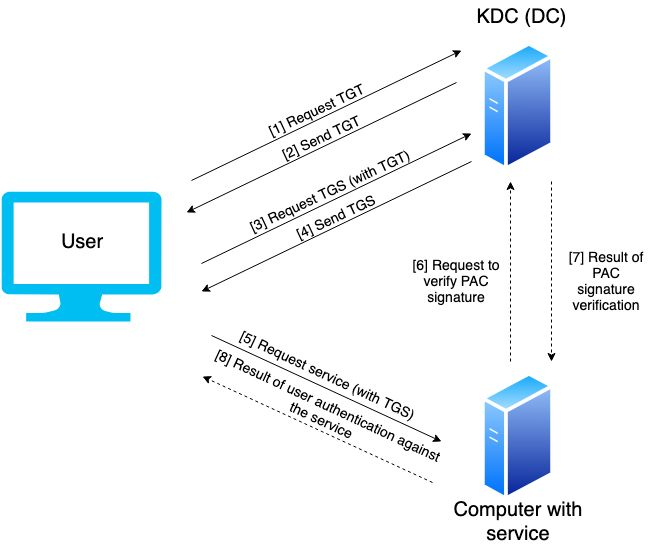
\includegraphics[width=.8\textwidth]{figuras/TGT_TGS_PAC.jpg}
	\caption{Steps for Kerberos authentication}
\end{figure}
\linej
The process to access a service is as follows\cite{tarlogic_theory}\cite{tarlogic_comprehension}\cite{events_1}:
\begin{enumerate}
	\item The user request a Ticket Granting Ticket (TGT). This ticket is encrypted with the KDC key and is used for request to the KDC one or more Ticket Granting Service (TGS). This request is ciphered with the user hash.
	\item The DC returns the requested TGT is everything is in order.
	\item The user requests the TGS.
	\item The DC returns the requested TGS is everything is in order.
	\item The user sends a request to a computer running a service to make use of it. For this the TGS is sent.
	\item Optionally the Privilege Attribute Certificate (PAC) can be sent to the DC to be verified. The PAC is an structure present in almost every ticket that contains the privileges of the user and it is signed with the KDC key. Nevertheless, the PAC verification checks only its signature, without inspecting if privileges inside of PAC are correct. Furthermore, a client can avoid the inclusion of the PAC inside the ticket by specifying it in KERB-PA-PAC-REQUEST field of ticket request. Unfortunately most services do not validate the PAC.
	\item Optionally the DC returns the result to the computer that requested it, which should be running the service in question.
	\item Optionally the user receives the response to his request to use the service.
\end{enumerate}

\linej
The Golden Ticket attack depends on obtaining the password information of the KRBTGT account to generate a forged TGT. It can provide the attacker with the desired privileges in the AD (like administrator).
\linej
This means TGTs can be generated to access every account within the AD. This forged TGT is known as Golden Ticket.
The Golden Ticket does not depend at all of the administrator password of the AD, which means that changing this password does not invalidate a Golden Ticket in anyway.
\linej
\linej
Because the attack uses a valid TGT is very hard to detect it is a forgery. Once it has been issued the TGT can be used at any time and any amount of times until the time expiration.
Any TGS obtained from a Golden Ticket is no longer a forgery, because is generated from the DC.
\linej
\linej
The password information of the KRBTGT account can be just the hash of the password, which is stored in memory and can be retrieved with enough local privileges in a DC. To generate the Golden Ticket the attacker also needs the domain name and the SID of the domain to which the KRBTGT account belongs, which are trivial to get\cite{stealthbits}.
\linej
Furthermore once the required data is obtained the Golden Ticket can be created offline using certain programs, like Mimikatz. This means is impossible to detect the creation of the ticket itself if is not done on a computer in the network.
\linej
It follows that this attack can only be detected either during the steps needed to create the TGT (get the hash of the KRBTGT account) or by the use of the TGT.
\linej
\linej
By default Mimikatz sets the forged ticket age to 10 years, which is useful to some attackers because they would need only one attack to compromise the entire network for that time.

\subsection{Exploit methods}
To keep this simple only the basics are explained about the techniques used in the examples for a Golden Ticket attack. Because some of the exploits are similar they are numbered for easier identification. The scripts in the next exploits were used to understand the different ways to perform Golden Ticket attacks and during the tests to try to detect them. Of course there are more ways to generate a Golden Ticket, and some are much more harder to detect, but there is no time to examine them all. Also it is possible to combine several of the next exploits or change some of their steps.
\linej
For example there is a sever-agent version of Mimikatz called Pypykatz\cite{pypykatz_agent}\cite{pypykatz_server} that is very new and should be a bit harder to detect that the exploits showed here. Unfortunately the student could not make it retrieve the KRBTGT hash.
\linej
\linej
These scripts try to automate as much of the process as possible, which is usually done in an interactive way. This automation helps to assure that the results are the same each time and reduces the time for each test. All the tests in this project were executed at least twice. Tests were repeated if there were changes that could affect their results.

\subsubsection{Exploit 1: Local Mimikatz in DC}
This requires local administrator privileges in the DC and also and an already downloaded version of Mimikatz in the DC, which the attacker can easily get after gaining privileges. If this example were to be used as it is it will probably be detected by the antivirus and Windows Defender, but again they can be disabled by a local administrator and there are techniques to avoid being detected by them.
\linej
\lstinputlisting[style=PS,caption=Script to generate and inject a Golden Ticket,captionpos=b]{src/genticket.ps1}
\linej
The script uses Mimikatz to get the needed data to generate the Golden Ticket, saving it to a file for convenience. Then the data is split in variables, each being a piece for generating the forged ticket. The \textit{exit} parameter is to exit the Mimikatz shell after executing the command.
\linej
After injecting the ticket (with the \textit{/ptt} option) the session haves administrator privileges in the AD, so any service in the AD can be used in this PowerShell session, any command should be allowed. Without the injection option Mimikatz would store the ticket in a file, which can be injected at any time with Mimikatz.
The id 500 is the normal id for the administrator account in the AD.
This script can be executed in multiple ways, for example from a PowerShell interactive terminal run as an administrator.
\linej
\lstinputlisting[style=txt,caption=Example of the contents of the output file,captionpos=b]{src/output.txt}
\linej
The password hash of the KRBTGT account is retrieved by Mimikatz interacting with the Local Security Authority (LSA) or Local Security Authority Subsystem Service (LSASS), which is run by the lsass.exe process.
\linej
This process is the Windows service responsible for providing single sign-on functionality.
With it users are not required to re-authenticate each time they access resources.
It provides access not only to the authenticated user's credentials, but every set of credentials used by every open session since the last boot\cite{wikipedia_lsass}\cite{dump_ways}.
\linej
Mimikatz exploits this cache of credentials and reports the results to the user in the various forms employed by LSASS\cite{SANS_mimikatz}\cite{pentestlab}.

\subsubsection{Exploit 2: Mimikatz from memory in DC} \label{invoke-Mimikatz}
This is similar to the previous example but instead of having a downloaded version of Mimikatz (stored in the disk) the program is downloaded directly into the PowerShell session, so Mimikatz is never stored in disk.
The clear advantage over the previous one is that it should be harder to detect.
\linej
With slight changes this could work in a computer that is not a DC, if the attacker compromised a workstation a domain admin logged onto\cite{dump_ways}.
\linej
\lstinputlisting[style=PS,caption=Script to run Mimikatz only in memory and inject a Golden Ticket,captionpos=b]{src/genticket_mem.ps1}
\linej
The script downloads a version of Mimikatz from Github and creates a PowerShell object with its contents, that can be invoked at any time in this shell\cite{powersploit}\cite{mimikatz_details}. Then as before it dumps the needed information to generate the Golden Ticket in a file, which is read and parsed to store the interesting parameters into variables.
\linej
Due to difficulties with the last \textit{Mimikatz} command to work with the parameters in the variables a workaround was used. This is writing a new file that has the command with those parameters, and then execute the file.
\linej
\linej
On the one hand it can be harder to detect with obfuscation, renaming and not using such an obvious url.
On the other hand PowerShell can be monitored for downloading commands, particularly those with objects.

\subsubsection{Exploit 3: Mimikatz with DCSync}
The DCSync is a Mimikatz feature in which a no-DC attempts to impersonate a DC and request account information from a real DC. This technique is less noisy because it does not require direct access to a DC (which are often heavily monitored)\cite{dump_ways}\cite{pentestlab}. To run Mimikatz we still need local administrator privileges in the computer.
\linej
\lstinputlisting[style=PS,caption=Script to run Mimikatz with DCSync,captionpos=b]{src/genticket_dcsync_mimikatz.ps1}
%some times the dcsync Mimikatz command does not work and needs to restart the no DC computer
\linej
This follows the same structure as the previous cases, but this time with the dcsync option.
The disadvantage in this case is that there needs to be a connection to a running DC that is not being monitored for the requests Mimikatz sends. There are open source tools available for this kind of monitoring\cite{dcsync_monitor} and it can also be detected by monitoring the network\cite{dcsync_monitor_network}.

\subsubsection{Exploit 4: DCSync with Kiwi}
In this case the access to the no-DC computer in the targeted network is done through Metasploit\cite{metasploit} and its own version of Mimikatz called Kiwi\cite{pentestlab}. The Kali virtual machine is for running Metasploit outside the AD, but a Windows machine running in the AD could have been used as well.
\linej
We need to know the password of the account we want to access remotely and the targeted computer needs to have a SMB share.
In this case the variable \textit{SMBPass} stores the password, which is \textit{Passw0rd}.
\linej
\lstinputlisting[style=ruby,caption=Part 1 of the remote DCSync exploit automation,captionpos=b]{src/metasploit_p1_kiwi.rc}
\linej
This runs a remote process, exploiting the SMB capabilities to run commands to spawn a Meterpreter shell\cite{meterpreter} with administrator privileges. There is a chance that the \textit{run} command fails to provide a Meterpreter shell at this stage, but trying again always ends working because the session is not getting created even though the exploit is working.
\linej
\linej
Now we are in a Meterpreter shell, which we can use to get the exact privileges we need for the next part. This is because even though we have administrator privileges there are different kinds of administrator privileges on Microsoft systems.
\begin{figure}[H]
	\centering
	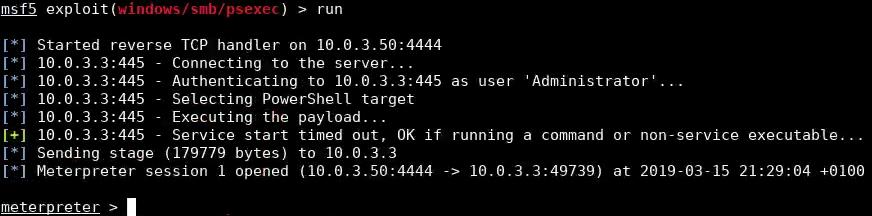
\includegraphics[width=\textwidth]{figuras/meterpreter.png}
	\caption{Meterpreter shell running}
\end{figure}
\linej
To do this we look for a session running administrator privileges in the AD. In this case the targeted machine had a PowerShell session running as administrator, to which we migrate.
\linej
\begin{figure}[H]
	\centering
	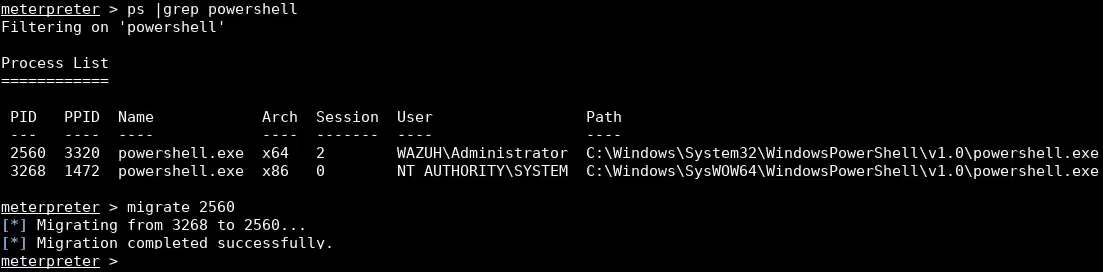
\includegraphics[width=\textwidth]{figuras/migrate.png}
	\caption{Migration to a PowerShell session as AD administrator}
\end{figure}
\linej
Now we are ready to run the real exploit. This loads the Metasploit version of Mimikatz (Kiwi) in the Meterpreter shell, allowing the attacker to use Kiwi commands.
The command in this case retrieves the information of the KRBTGT account needed to generate the Golden Ticket.
\linej
In this case the generation of the ticket is not using the data in an automated way, because there was no real need since is the same every time and the time needed to do this with Ruby felt like a waste. In this case the ticket is saved to the \textit{/tmp/golden.tck} file in the Kali machine.
\linej
\lstinputlisting[style=ruby,caption=Part 2 of the remote DCSync exploit automation,captionpos=b]{src/metasploit_p2_kiwi.rc}
\begin{figure}[H]
	\centering
	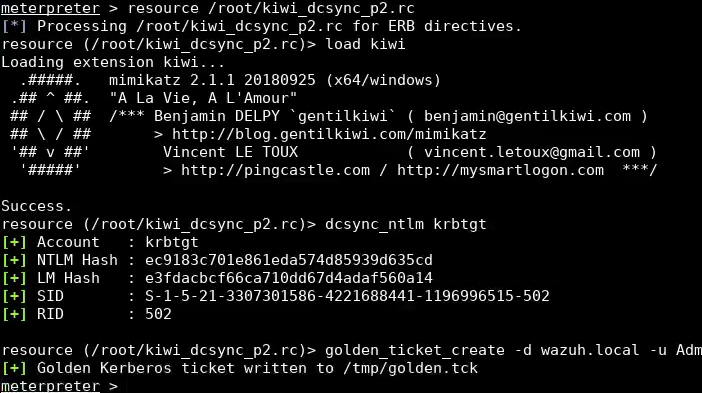
\includegraphics[width=\textwidth]{figuras/kiwi_p2.png}
	\caption{Retrieval of KRBTGT data and generation of the Golden Ticket with Kiwi}
\end{figure}
\linej
The obvious downside of this method for the attacker is that Metasploit is very widely used and known, therefore there could be security monitoring for it\cite{detect_metasploit_traffic}. But again the attacker is using a technique that does not need to control a DC and does not need to store anything in the disk of the targeted system, making it much harder to detect in that regard.
\linej
\linej
Of course there is no real need to use Metasploit to get a remote shell to run Mimikatz. The attacker could use ssh, run remote commands with \textit{psexec} or use the Windows Remote Shell. But some of these need to be enabled and they would not be much different of the previous examples.

\subsubsection{Exploit 5: Hashdump with Meterpreter}
Using a reverse TCP exploit the attacker access the targeted DC with a Meterpreter shell. This is similar to the previous case but using the Meterpreter command \textit{hashdump} instead of the DCSync retrieval of Kiwi\cite{pentestlab}. This stills uses Kiwi to generate the Golden Ticket.
\linej
\lstinputlisting[style=ruby,caption=Part 1 of the remote Hashdump exploit automation,captionpos=b]{src/metasploit_p1_hashdump.rc}
\linej
Again there is a migration to an administrator account of the AD. In this case another command to get the SID of the network would be needed if we did not know it already, for example a simple \textit{whoami /user} would suffice.
\linej
\lstinputlisting[style=ruby,caption=Part 2 of the remote Hashdump exploit automation,captionpos=b]{src/metasploit_p2_hashdump.rc}
\begin{figure}[H]
	\centering
	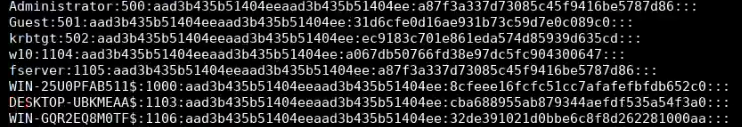
\includegraphics[width=\textwidth]{figuras/hashdump.png}
	\caption{Retrieval of KRBTGT data with hashdump}
\end{figure}
\linej
As before it is expected of the DCs to be more monitored. This means that the DCSync version is more interesting to an attacker because it has the same difficulty and benefits at a lower risk.

\subsection{Detection purely with signatures}
Searching for suspicious strings can be used to trigger alerts with Wazuh.
Signature matching of data coming from Windows events and default logs from Windows systems is not much different from what any antivirus do. It follows that it would be as easy to evade as them. For example with substitution of suspicious strings from the source code and recompilation\cite{understanding_powersploit_mimikatz}.
\linej
\linej
This does not mean that signature matching is totally worthless, but that it is not something to focus on. In this project relying in signatures was avoided as much as possible.
Useful signatures to match not only amount to third-party tools. It is easy to monitor extensions, directories, certain files, command line options, usernames, etc.
\linej
Obviously matching some signatures is more valuable than matching others. For example finding \textit{Mimikatz.exe} is easier to implement and less valuable than \textit{krbtgt}, \textit{lsadump}, \textit{kerberos::} or \textit{privilege::}.
\linej
\linej
As we know the techniques to detect or avoid detection evolve with each other over time.
Any way we manage to detect programs like Mimikatz could be overcome in the future.
\linej
That does not mean that detection techniques are bound to fail or that there is no point to them.
Many attackers know how hard it can be to overcome detection techniques.
\linej
It is also important to remember these scenarios are continuously changing, with new techniques to avoid detection and the creation of new tools.

\subsection{Detection purely with Windows events}
In theory we can identify certain attacks only with the security events of Windows. There are multiple websites in which this attack has been analyzed and its events identified\cite{events_1}\cite{detection_events}.
\linej
Unfortunately the events recorded did not always probe to be the same as the cited sources (probably because it was tested on the new Windows Server version, 2019).
In most cases their frequency is not enough to be distinguished of the regular activity, even when using a lab environment without work load.
This could probably be improved if these events had more information (particularly those as critical as Kerberos'), but they are very short and generic.
\linej
\linej
Wazuh provides access to Windows events by default, due to the rules and decoders of its ruleset\cite{wazuh_ossec_ruleset}, the user only needs to define rules to specify what and how he wants to monitor.
\linej
We can enable additional logging with the Advanced Audit Policy Configuration. For example for auditing kernel objects, more Kerberos logging, changes in settings or account events.
\linej
\linej
The student tried to analyze the security events to find patterns in the previous exploits, by recording all the data received by Wazuh in during their execution. This was done just by looking the current line of the log, executing the exploit and copying the log from there to a new file.
\linej
The obvious problem of this method is that it results in logs with tens to hundreds of lines filled with a not very easy to read format. The workaround used was to parse the logs with custom AWK scripts\cite{memoria_github}, removing fields to make the logs more readable and counting each of the events in them.
\linej
\linej
The idea of finding a relationship between certain windows events and this attack was abandoned because:
\begin{itemize}
	\item It was not providing any new results.
	\item It was too time consuming.
	\item It can be accomplished using Sysmon\cite{sysmon}\cite{sysmon_event_7_mimikatz}.
	\item Also it was concerning the amount of noise this method has, even though in a laboratory without real system load, to tell apart an intrusion from a totally healthy system.
\end{itemize}
\linej
The real useful addition to the Windows builtin events is having Sysmon\cite{sysmon} in each of the monitored Windows computers. They can be combined to identify attackers better\cite{detection_events}.
\linej
With Sysmon we can have reports of events [1-21] and 255, which in some cases provide very precise and useful information of the system. For example we can configure Sysmon to log data about process with a certain processes, like: \textit{PowerShell}, \textit{Mimikatz}, any \textit{.ps1} or any \textit{.exe}.
Sysmon can monitor each of the events either by whitelisting or blacklisting by default or both. We can also combine it with rules from Wazuh, using Sysmon to increase the report capabilities and Wazuh to filter them.
\linej
\linej
\label{increment_explanation}
Originally getting more data from Sysmon and other sources for detection was an increment in itself, but seeing as the first increment could not be accomplished without it both were combined into the same increment.
This was due to overestimating the report capability of Windows events in the planning stage and because increment 2 was way easier than planned.
From this point Sysmon and remote scripts are used to identify threats and they do not have to be just additional detection as it was first planned.
\linej
\linej
Also is important to note that Sysmon can be a bit tricky to balance the configuration to get as much suspicious events as possible, while not reporting so much it affects the performance of the network. This is responsibility of the administrators of the network, who also have to tune the configuration to their custom needs.
There are public configs for Sysmon that attempt to provide a good insight of the system while not logging too much data\cite{sysmon_config} and some even with OSSEC on mind\cite{ossec_sysmon}.
\linej
\linej
Having a working setup of Wazuh and Sysmon just requires to install Sysmon in the Windows computers and enable forwarding its log \ref{lst:forward_sysmon}.

\subsection{Detection of Mimikatz}
Mimikatz is the tool of choice for this kind of attack for most attackers because it is very effective, easy to use and has multiple ways to be used in different attacks\cite{mimikatz_github}\cite{mimikatz_details}. This is a double edge sword for Mimikatz because it has become one of the programs to look for in antimalware detection programs. In this case we assume these programs have not detected Mimikatz and is up to Wazuh to do it. It is interesting to note that the author of Mimikatz provides ways to detect it, like the YARA rules he maintains\cite{mimikatz_github} or BusyLights\cite{understanding_powersploit_mimikatz}.
\linej
\linej
Detecting Mimikatz is not a sign of a Golden Ticket attack (unless is clear in the way it is used), but still it is a big and dangerous threat to the system and worth checking out.
\linej
Unfortunately as seen in the exploits before there are multiple ways to execute Mimikatz, in an attempt not to be discovered by known techniques.
\linej
\linej
Each time a Mimikatz shell spawns certain DLLs are loaded. The technique to identify a succession of events in a short time as another event is called grouping or composite.
Grouping is a very effective technique, but it can require a lot of work to identify its components. In some cases the attack may not produce enough noise or it may not be possible to tell it apart from the normal events of the system\cite{sysmon}\cite{sysmon_event_7_mimikatz}.
\linej
Fortunately Mimikatz needs a fair amount of DLLs to work and some of them are not very usual. This makes the execution of Mimikatz noticeable.
\linej
\linej
 The load of a DLL can be detected by the event 7 of Sysmon and the grouping can be identified with Wazuh rules. It also can be detected by the event 10 of Sysmon, for inter-process access, but a greater cost of bandwidth.
For this task is better to configure Sysmon to monitor these 5 images, to avoid logging too much:
\linej
\lstinputlisting[style=xml,caption=Sysmon monitoring with event 7 for certain DLLs,captionpos=b]{src/sysmon_event_7.xml}
\linej
On the manager side the next rules are needed:
\linej
\lstinputlisting[style=xml,caption=Rules for suspecting a Mimikatz execution as a group of events,captionpos=b]{src/rules_event_7_mimikatz_alternative.xml}
The \textit{sysmon\_event7} means that another rule has marked the log as a Sysmon event of type 7.
\linej
The \textit{same\_field} option means that every one of the matches must have the same value in the designed field, which in this case means that these events come from the same computer.
\linej
The \textit{frequency} option means that the rule has to be matched that number of times to trigger. Is set to 2 because is the minimum value possible.
\linej
\linej
Usually each of the suspicious DLLs would have its own rule, but it would not always identify Mimikatz because the frequency has to be at least 2. Therefore rules \textit{300301} and \textit{300302} identify 2 and 3 DLLs each (using a logical OR), making it possible to trigger the grouping rule.
The last rule identifies the use of the DLLs in a 10 seconds gap as the execution of Mimikatz. This detection could be evaded by adding time between the load of the DLLs in the source code.
\linej
\linej
The problem of these less precise rules is that it is possible to have false positives. None were seen during this project for this case.
\linej
Unfortunately due to the way OSSEC matches rules there is no way to have an hierarchy of rules to trigger a precise grouping rule or the other one.
\linej
\linej
Detecting the use of every variant of Mimikatz is virtually impossible, not only because their sheer number due to its popularity but because anyone can compile their own. Therefore the logical way to detect Mimikatz would be to detect the basic step for every version: the interaction with the LSASS and process injection. More can be read on page \pageref{detect_lsass}.

\begin{table}[H]
	\centering
	\begin{tabular}{|l|l|}
		\hline
		\rowcolor{gray!30}
		Exploit & Detected \\ \hline
		1: Local Mimikatz in DC& \RYES\\ \hline
		2: Mimikatz from memory in DC& \RYES\\ \hline
		3: Mimikatz with DCSync& \RYES\\ \hline
		4: DCSync with Kiwi& \RYES\\ \hline
		5: Hashdump with Meterpreter& \RYES\\ \hline
	\end{tabular}
	\caption{Exploit detection by grouping events}
\end{table}
This method detects the use of Mimikatz in all the ways implemented in this project.
The hashdump exploit is detected because Kiwi is used in the session in that machine to generate the Golden Ticket. A real attacker probably would generate the ticket outside of the network, avoiding being detected by this technique.

\subsection{Detection of the use of the TGT with klist} \label{klist_detection}
We can not always detect when a forged TGT is generated, but the attacker still needs to use it to gain access to the active directory domain with the privileges set in the ticket. The first choice for this task would be to monitor the Kerberos log searching for unusual patterns, but it proved to be more hard than it should, so instead a scan the cache of Kerberos tickets every few minutes was implemented.
\linej
The program to examine the contents of the cache is \textbf{klist}.
\linej
\linej
In order to do this we need to enable the execution of Wazuh's remote commands in the Windows agent and set the properties of the command in the manager \ref{lst:klist_wodle}\cite{wazuh_remote_command}.
\linej
\linej
In this case the command is a script \ref{lst:klist}\ to get all the tickets of all the sessions with klist, compare the ticket value for the field \textit{TicketExpireHours} with the value of \textit{MaxTicketAge} of the Group Policy (putting the difference in a new field) and parse the output to JSON. Having the output in JSON makes it a bit easier to read from the logs (which is useful to fix any mistake in the script) and removes the need of a decoder in the manager.
The idea came from a very different klist script that only works interactively and reports in plain text\cite{klist_script_idea}.
\linej
This script needs to be run in every member of the network to guarantee detection for every user.
\linej
The conversion to JSON was done manually to add information and because the ``ConvertTo-Json'' cmdlet does not work as expected.
Doing this with only PowerShell assures it will work in any Windows system without external programs. The downside of this parsing and my limited knowledge of PowerShell is that the script is a bit bulky and the dependency on the format of the output of klist.
\linej
\linej
Unfortunately the automated way to get the \textit{MaxTicketAge} from the Group Policy in \ref{lst:klist_getMaxTicketAge}\ does not work by default with remote commands because Windows remote commands only allow certain types of commands.
In any case the \textit{MaxTicketAge} value is not usually changed and it requires AD administrator privileges to do it, so due to the time constrains of the project this automation was abandoned. There are other ways to get the \textit{MaxTicketAge} value, but as mentioned is not something to spend time on.
\linej
\linej
Next there is an example of the difference between the normal output of klist and the string stored in an alert in the manager.

\begin{figure}[H]
	\centering
	\includegraphics[width=.9\textwidth]{figuras/klist_normal.png}
	\caption{Klist listing tickets for a certain session}
\end{figure}
\begin{figure}[H]
	\centering
	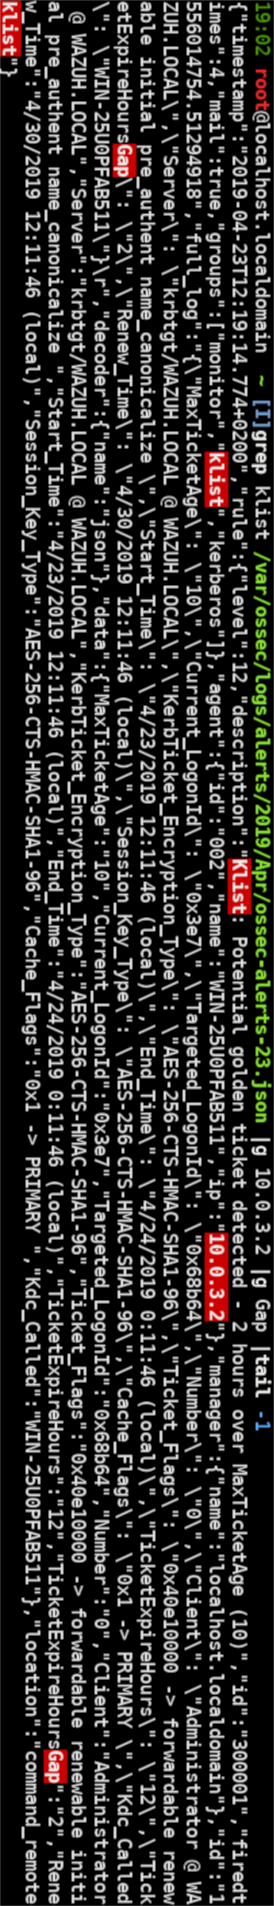
\includegraphics[height=\textheight]{figuras/klist_alert_rotated.png}
	\caption{Latest alert of the klist monitoring in the manager}
\end{figure}
\linej
The time difference mentioned before is a very easy way to detect a forged ticket. With a simple subtraction in the PowerShell script only a rule that makes a number comparison in the manager is needed to launch the alert.
\linej
\lstinputlisting[style=xml,caption=Rules to detect a suspicious expiration age from the report of the klist script,captionpos=b]{src/rules_klist.xml}
\linej
The purpose of the first rule is to identify any log in JSON with \textit{MaxTicketAge} and \textit{TicketExpireHours} fields. The second rule is used to examine the contents of the \textit{TicketExpireHoursGap} field of the logs that the first rule has identified. If the value of the \textit{TicketExpireHoursGap} field starts with a digit different than 0 then it means that \textit{MaxTicketAge} $>$ \textit{TicketExpireHours}, therefore the expiration age is greater that it should, triggering an alert.
Additionally it can only trigger once each 600 seconds, to avoid flooding of alerts.
\linej
\linej
This attack is often used because it may grant the highest privileges in the domain, is hard to detect and is very persistent because it does not care for the password changes in the active directory. That is why is very attractive for domains in which the attacker may decide to come back later, maybe even years later. That means is very unlikely for a forged ticket to not have a very big expiration age, because is one of its most appealing benefits; but again it would be possible to an attacker to keep generating forged tickets with a valid expiration age forever, at a greater risk of being detected in other ways.
\linej
\linej
The testing of the script was satisfactory, the cases that inject a TGT were detected and there were no false positives:
\begin{table}[H]
	\centering
	\begin{tabular}{|l|l|l|}
		\hline
		\rowcolor{gray!30}
		Exploit & Detected & As expected \\ \hline
		1: Local Mimikatz in DC& \RYES& \RYES\\ \hline
		2: Mimikatz from memory in DC& \RYES& \RYES\\ \hline
		3: Mimikatz with DCSync& \RYES& \RYES\\ \hline
		4: DCSync with Kiwi& \RNO& \RYES\\ \hline
		5: Hashdump with Meterpreter& \RNO& \RYES\\ \hline
	\end{tabular}
	\caption{Exploit detection by the klist script}
\end{table}
Of course if we chose to store the ticket in a file we could inject it in other moment or computer, but then it could be detected by this method.
\linej
\linej
Additionally there could be monitoring for unusual usernames, because is possible to get a TGT with administrator privileges with non existent username to avoid the monitoring that administrator accounts are often under.
\linej
\linej
It can be worth checking if the attacker is using klist to clean the cache of injected tickets, to cover any tracks. This can be easily accomplished monitoring the execution of klist with the event 1 of Sysmon:
\begin{lstlisting}[style=xml]
<ProcessCreate onmatch="include">
	<Image condition="contains">klist</Image>
</ProcessCreate>
\end{lstlisting}
\linej
And checking with Wazuh if the option \textit{purge} was used:
\lstinputlisting[style=xml]{src/rules_klist_purge.xml}

\subsection{Silver Ticket}
A Silver Ticket is very similar to a Golden Ticket, is a forged TGS instead of TGT. Therefore a Silver Ticket only grants access to a service in a computer. Is important to note that some services need the privileges of more services, therefore more than a Silver Ticket may be needed.
\linej
Steps 1 and 2 of a normal Kerberos authentication exchange are not needed (figure \ref{kerberos_exchange}) because they are only to get a TGT. Without a TGT a TGS can not be requested from the DC, so steps 2 and 3 are also not a part of the Silver Ticket attack.
\linej
There is no need to connect to a DC, only a connection to the computer hosting the service is needed (steps [5-8]). Unless PAC validation is required, the service accepts all data in the TGS ticket.
\linej
The TGS is ciphered with the password hash of the account running the service, making changes of the password an effective mitigation against Silver Tickets.
To extract this data from memory the attacker has to have local administrator privileges\cite{events_1}\cite{silver_ticket}.
\linej
\linej
To extract the data the attacker would need to run Mimikatz with:
\begin{lstlisting}[style=PS,numbers=none]
"privilege::debug" "sekurlsa::logonpasswords" exit
\end{lstlisting}
\linej
For example in the next scenario:
\begin{itemize}
	\item The user to impersonate is the AD Administrator.
	\item The computer is is \textit{WIN-GQR2EQ8M0TF}.
	\item The domain is \textit{wazuh.local}.
	\item The domain is identified as \textit{S-1-5-21-3307301586-4221688441-1196996515}.
	\item The attacker wants access to the \textit{HOST} service.
	\item The password hash of the account is \textit{68fbd238f574f7685beed96a2db15004}.
\end{itemize}
The Mimikatz command would be:
\begin{lstlisting}[style=PS,numbers=none]
"kerberos::golden /admin:Administrator /id:500 /sid:S-1-5-21-3307301586-4221688441-1196996515 /domain:wazuh.local /target:WIN-GQR2EQ8M0TF.wazuh.local /rc4:68fbd238f574f7685beed96a2db15004 /service:HOST /ptt" exit
\end{lstlisting}
Allowing the attacker to access the \textit{HOST} service on that computer with AD Administrator privileges.
\linej
\linej
Silver Tickets get registered in the Kerberos' cache in the same way as the Golden Tickets, so they can be detected with the klist script. The execution of Mimikatz can be detected with grouping just as before.

\subsection{Mitigation}
These exploits take advantage of the inherent weaknesses of Kerberos, so there is no way to fully prevent them. Nevertheless, Microsoft provides a public guide explaining how to mitigate this kind of attacks\cite{microsoft_mitigation}.
The easiest way to mitigate this attack is to change the password of the KRBTGT account to invalidate any existing Golden Ticket, which has to be done twice (make sure the domain converges before doing the second password change\cite{hood}), but it also invalidates existing proper TGTs.
\linej
The recommendation from Microsoft is to regularly reset the password\cite{tarlogic_comprehension}\cite{adsecurity_483}, which can be done with their official script\cite{reset_script}. This could be also triggered by alerts that we are confident detect Golden Tickets, but as mentioned this could affect other functionality and so the decision is for the network administrators to make. Any TGT that is not valid produces an error in a TGS request, which can be used for exposing an attacker\cite{scom_GT}.
\linej
\linej
Also there are other measures like:
\begin{itemize}
	\item Have administrative passwords longer than 25 characters to avoid brute force cracking and make them unique for each system.
	\item Enforce a least privilege model.
	\item Minimize the quantity of administrative accounts.
	\item Isolate DCs: Use DCs only as servers, never work stations of any kind.
	\item Isolate administrator accounts: Use administrator accounts only for administrator duties.
	\item Isolate AD accounts: Create tiered groups with very granular permissions on the domain and create Access Control List permissions on the Organization Units of the AD\cite{AD_tier}.
	\item Use Read Only Domain Controllers (RODCs): keep Read Write DCs segregated using network segregation and AD sites to force users to logon to RODCs, making breach detection easier. RODCs don't have any real user hashes (nor the hash of the KRBTGT account)\cite{hood}\cite{reset_RODC}.
	\item Use honeypots: With populated the LSASS cache with false credentials\cite{SANS_mimikatz}\cite{honeyhashes} or with decoy AD objects\cite{decoy_AD}. And then monitor the logs for attempts to use them. This can lead to detect attackers or to find vulnerabilities in the network.
	\item Disable storage of clear text passwords in LSASS memory to limit the information provided by Mimikatz\cite{SANS_mimikatz}.
	\item Run LSASS in protected mode (from Windows 8.1): calls to LSASS are only allowed by other protected-mode processes\cite{SANS_mimikatz}\cite{understanding_powersploit_mimikatz}.
	\item Use choke points: Create a choke point for access to your DCs, adding another layer of protection. Create a Terminal Server that can only talk to the DCs. Configure the DCs to only accept administrative connections from that Terminal Server\cite{choke}.
\end{itemize}
\linej
We could go on with more detail and increasing the mitigation\cite{AD_defense}, but is not the objective of this project.

\subsection{Conclusion}
We have seen how the data to generate Golden Tickets can be obtained in different ways and the difficulties for both the attacker and the defender roles.
\linej
\linej
Relying on the klist detection means there is no real need to detect each of the different ways to generate the Golden Ticket because it may be impossible depending on the circumstances. More importantly the attacker still needs to present it to a DC to get the TGSs, to get any benefit from the Golden Ticket.
\linej
Detecting certain Sysmon events in a close time gap can guarantee the detection of Mimikatz, therefore detecting one of the most used ways to gather this data. Detecting certain signatures for running commands, reads and accesses are a worthy way to detect the creation of a Golden Ticket, without spending much resources.
\linej
These are good examples of how detecting common steps to multiple exploits is one of the strong points of an HIDS.
\linej
\linej
Another way of detection is to use YARA to look for certain patterns in memory, just like we can search for strings in the events. In the case of events the data comes from the program, which is easy to modify with multiple techniques like substitution or obfuscation. The patterns in memory are much more harder to change because it involves changing the logic of the program. That means most attackers would just take the risk to be detected by this kind of technique.


\section{More about the extraction of credentials}
In the previous section the extraction of credentials was explained to understand the details surrounding a Golden Ticket attack. This includes extracting password hashes from the memory of the LSASS process with Mimikatz or Hashdump. But there are more ways of extraction that are used against AD network now a days.
\linej
Once credentials have been retrieved an attacker has more options, like generating a Golden Ticket.
The key points of access are the \textit{NTDS.DIT} file that is stored in disk and the running process \textit{lsass.exe}.

\subsection{Exploit methods}
Because the database file of the AD accounts is locked from copying and reading, only Windows tools are allowed to. These tools are \cite{dump_ways}:
\begin{itemize}
	\item Reg: Allows to change or save registry hives, including those that contain credentials.
	\item Ntdsutil: Provides management of this database, including creation of backups.
	\item WMIC: Commands for the Windows Management Instrumentation. They allow all kinds of remote management, including copy of files using Shadow Copy. Sysmon has 3 events to monitor them specifically.
\end{itemize}
Another way to extract these credentials is to dump them from memory using third party tools and scripts. This is saving part of the data of a process running in the system\cite{dump_ways}.
There are multiple tools available for this, but in this project only these were used: Mimikatz, Hashdump, ProcDump, pd, Minidump.
\linej
Some of these tools have the option to retrieve the password or hashes history, meaning that the attacker could gain valuable insight on the password policy of the target.
\linej
\linej
There was no effort to automate these exploits because they are too simple.
All the extraction programs were executed with local administrator privileges in a DC.

\subsubsection{Exploit 6: Retrieval of NTDS.DIT with ntdsutil}
Another way to get the desired information is to copy the database of the AD Domain Services (the NTDS.DIT file) and conduct an offline password audit of the domain. This means once we have this data we can use a wide selection of tools to crack it\cite{ntdsdit_tools}\cite{extracting_ntds}\cite{ntds_powershell}.
\linej
\linej
The attacker has to open a shell as administrator in a DC to create the backup. Multiple commands or an one-liner can be used:
\begin{lstlisting}[style=PS]
ntdsutil "activate instance ntds" ifm "create full C:\temp\ntdsutil" quit quit
\end{lstlisting}
\linej
This command creates a ntdsutil shell and activates the instance to later create a backup in a temporary directory (inside the ifm subshell).
\begin{figure}[H]
	\centering
	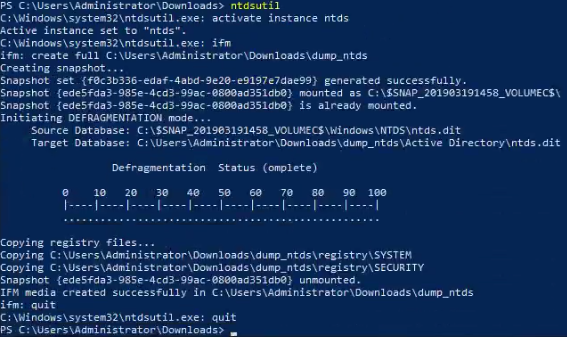
\includegraphics[width=\textwidth]{figuras/ntdsutil.png}
	\caption{Backing up the database of the AD using the ntdsutil shell}
\end{figure}
\linej
There are other ways to use ntdsutil in ways harder to detect\cite{more_dumps}, but this is enough for gathering events for analysis.
\linej
\linej
The creation of processes related to ntds can be reported by Sysmon:
\begin{lstlisting}[style=xml]
<ProcessCreate onmatch="include">
	<Image condition="contains">ntdsutil.exe</Image>
</ProcessCreate>
\end{lstlisting}
\linej
And alerts set with Wazuh:
\label{ntdsutil_detection}
\lstinputlisting[style=xml]{src/rules_ntds.xml}
\linej
The first rule is the parent, it filters windows events with the \textit{ntds} string.
\linej
The second rule detects the ntdsutil executable. This signature is more useful than normal because it is a builtin tool. The third matches \textit{ntds} for the command line, which is not really reliable.
\linej
The rest are for detecting suspicious database events from Windows events. These database events assure the detection of ntdsutil even if it were to be executed without using known signatures.
\linej
\linej
There is also the remote version of Reg: WinReg. But there was no time to investigate on it. Is likely that it can be detected with network monitoring, as other remote tools.

\subsubsection{Exploit 7: Storing registry hives with Reg}
These commands produce the different save files, each of a different group of credentials, that can be later extracted offline with certain tools\cite{more_dumps}:
\begin{lstlisting}[style=PS]
reg.exe save hklm\sam c:\temp\sam.save
reg.exe save hklm\security c:\temp\security.save
reg.exe save hklm\system c:\temp\system.save
\end{lstlisting}
\linej
Reg is not detected as malware because it is a builtin tool in Windows. With Sysmon we can report the execution of Reg with the event 1, reporting the creation of a process:
\begin{lstlisting}[style=xml]
<ProcessCreate onmatch="include">
	<Image condition="contains">reg.exe</Image>
</ProcessCreate>
\end{lstlisting}
\linej
And Wazuh to trigger an alert:
\lstinputlisting[style=xml]{src/rules_reg.xml}
\linej
The parent rule matches the creation of Reg from the report of Sysmon.
\linej
The second rule detects the \textit{save} string in the reg command.
\linej
The rest of the rules detect the registry strings for credentials.
\linej
\linej
This also could be detected using the event 7, but it would interfere with grouping detection. Of course it is possible that these rules do not cover all the extraction uses of Reg. Is worth noting that this is a signature base detection, therefore it could be overcome with certain third-party programs.
\linej
\linej
Additionally a grouping detection for the DLLs Reg uses was tested. It detected Reg events every time without relying on the \textit{reg.exe} signature, but there were false positives, particularly during boot.

\subsubsection{Exploit 8: Dump of LSASS with ProcDump}
ProcDump\cite{procdump} is a command-line utility whose primary purpose is monitoring an application for CPU spikes and generating crash dumps during a spike. This program can be used to create a dump file of the running \textit{lsass.exe} process:
\begin{lstlisting}[style=PS,numbers=none]
C:\Users\Administrator\Downloads\procdump.exe -accepteula -64 -ma lsass.exe c:\temp\lsass.dmp
\end{lstlisting}
\linej
The dumped file can be used to extract the credentials by other programs, like Mimikatz\cite{more_dumps}. This is also true for the next exploits.

\subsubsection{Exploit 9: Dump of LSASS with pd}
ProcessDumper, also known as pd\cite{pd}, is another program to dump the \textit{lsass.exe} contents. For example if the id of the process is 552:
\begin{lstlisting}[style=PS,numbers=none]
C:\Users\Administrator\Downloads\pd.exe -p 552 > c:\temp\lsass.dump
\end{lstlisting}

\subsubsection{Exploit 10: Dump of LSASS with Minidump}
Minidump is a script from the PowerSploit Post-Explotation Framework\cite{powersploit}. It can be combined with the \textit{Get-Process} builtin to dump the process into a file:
\begin{lstlisting}[style=PS]
Import-Module c:\users\administrator\downloads\PowerSploit-master\Exfiltration\Out-Minidump.ps1
Get-Process lsass | Out-Minidump -DumpFilePath c:\temp
\end{lstlisting}

\subsubsection{Exploit 11: Retrieval of NTDS.DIT with NinjaCopy} \label{invoke-NinjaCopy}
%%fixes needed
%%	%https://github.com/PowerShellMafia/PowerSploit/commit/bd6fe64316afe293d6b4cdf095ed3cfb64b6ab25
%%	%https://github.com/PowerShellMafia/PowerSploit/issues/293
Another PowerSploit module that can be used to steal the NTDS.DIT file is \textit{NinjaCopy}:
\begin{lstlisting}[style=PS]
Import-Module C:\Users\Administrator\Downloads\PowerSploit-master\Exfiltration\Invoke-NinjaCopy.ps1
Invoke-NinjaCopy -Path "c:\windows\ntds\ntds.dit"  -LocalDestination "c:\temp\ntds.dit"
\end{lstlisting}
\linej
Or to copy the NTDS.DIT of the DC in this laboratory to a no-DC computer:
\begin{lstlisting}[style=PS]
Import-Module C:\Users\Administrator\Downloads\PowerSploit-master\Exfiltration\Invoke-NinjaCopy.ps1
Invoke-NinjaCopy -Path "c:\windows\ntds\ntds.dit"  -LocalDestination "c:\temp\ntds.dit" -ComputerName "WIN-25U0PFAB511"
\end{lstlisting}
\linej
This module allows any file, even if it is locked, to be copied without starting suspicious services or injecting in to processes. This is because it can copy \textbf{any file} from a NTFS volume, by opening a read handle to the entire volume, therefore bypassing the following protections\cite{dump_ways}:
\begin{itemize}
	\item Files which are opened by a process and cannot be opened by other processes, such as the NTDS.dit file or SYSTEM registry hives. This is known as locking the file.
	\item Flags set on a file to alert when the file is opened. Windows can not set a flag because NinjaCopy does not use a Win32 API to open the file.
\end{itemize}
\linej
The code to parse NTFS is loaded with a reflective DLL, making it harder to detect because it does not use the Windows loader nor a DLL file.
\linej
The direct read of the device can be reported with the event 9 of Sysmon, but event 1 can be useful to make sure in the remote case. This needs to be in the configuration file of Sysmon in the DC:
\begin{lstlisting}[style=xml]
<ProcessCreate onmatch="include">
	<Image condition="contains">wsmprovhost.exe</Image>
</ProcessCreate>
<RawAccessRead onmatch="include">
	<Image condition="contains">powershell.exe</Image>
	<Image condition="contains">wsmprovhost.exe</Image>
</RawAccessRead>
\end{lstlisting}
\linej
\lstinputlisting[style=xml,caption=Rules for detecting NinjaCopy,captionpos=b]{src/rules_ninjacopy.xml}
\linej
The local case only generates an event of type 9 and its only signatures are \textit{PowerShell} and \textit{Device{\textbackslash}HarddiskVolume}. It does not even record the name of the file because the handle is for the volume. This can not really guarantee this event comes from the execution of NinjaCopy, but until now has always worked and never reported a false positive. This rule could be much more useful if the NTDS.DIT file were in a different volume than normal.
\linej
\linej
The remote case is much more easier to detect. In the tests it spawned at least 4 events of each type in about 12 seconds, all from the DC.
The bigger the NTDS.DIT file and the slower the connection the more events are produced.
\linej
The remote command is executed by the \textit{wsmprovhost} program, which stands for Windows Remote PowerShell Session.
The contents of the logs of the event type 1 are easy to distinguish from normal, due to the constant value of the \textit{commandLine} and \textit{parentCommandLine} fields.
\linej
The second and third rules detect the events of type 1 and 9 for the remote execution, and the last rule is a grouping rule of these two. This assures there are no false positives, but the second rule matches the exploit so well that it could be left out and probably would never cause false positives.
\linej
If the remote command is executed from DC and set to copy from the same computer it still triggers the remote alert.
\linej
\linej
Grouping the DLLs loaded by the \textit{Import-Module} command probed to be effective. As with Mimikatz, this loads the DLLs needed for NinjaCopy to work, which can be registered by the event 7 of Sysmon:
\lstinputlisting[style=xml]{src/sysmon_event_7_ninjacopy_import.xml}
\linej
These 8 DLLs are detected by 4 rules to reach the minimum frequency:
\lstinputlisting[style=xml]{src/rules_ninjacopy_import.xml}
\linej
This detection works with both local and remote cases the same.
\linej
False positives were found when attempting to log in remotely multiple times one after the other, as described on page \pageref{reverse_login}.
Others may appear in a real environment.
This technique depends too much on the time frame and can be avoided changing the code.
%\linej
%\linej
%The next detection attempt was to use a grouping technique for the DLLs the program uses during the copy process. All of them were monitored with the event 7 of Sysmon. The most frecuent were: advapi32, kernel32, kernelbase, msvcrt and ntdll.
%\linej
%These DLLs are used very often in any healthy system. The script did not increase their use too much, therefore false positives were produced during normal execution, discarding this method of detection.

\subsection{Detection of process accessing LSASS} \label{detect_lsass}
The event 10 of Sysmon reports when a process access another process, possibly detecting hacking tools that read the memory contents of processes\cite{sysmon}.
This event can be used to detect LSASS dumps\cite{sysmon_event_10_lsass}.
\linej
The downside is it can generate significant amounts of logging, therefore it was configured to log only the LSASS process and exclude the instances from the OSSEC agent and the Virtual Box service.
%This exclude seems to affect other events of type 7 too, even though it should not.
\linej
\begin{lstlisting}[style=xml,caption=Sysmon monitoring with event 10 for LSASS reads,captionpos=b]
<ProcessAccess onmatch="include">
	<TargetImage condition="contains">C:\Windows\System32\lsass.exe</TargetImage>
</ProcessAccess>
<ProcessAccess onmatch="exclude">
	<SourceImage condition="contains">C:\Windows\System32\vboxservice.exe</SourceImage>
	<SourceImage condition="contains">C:\Program Files (x86)\ossec-agent\ossec-agent.exe</SourceImage>
</ProcessAccess>
\end{lstlisting}
\linej
After some analysis of these events it was clear that normal accesses could be identified by the \textit{grantedAccess} field. Its value is a mask, that indicates the type of privileges the process is accessed with.
\linej
They had a value of \textit{0x3000} (even though these do not happen often) or \textit{0x1000} if the process is \textit{svchost.exe}. The detected malicious programs produced at least one event with a different value on this field.
\linej
\lstinputlisting[style=xml,caption=Rules to detect unusual values of grantedAccess,captionpos=b]{src/rules_lsass.xml}
\linej
The first identifies events of type 10 for the LSASS process.
\linej
The second rule triggers if the string \textit{UNKNOWN} is in the field \textit{callTrace}. This occurrence was found during testing of the exploits 4 and 5, that use a reverse TCP shell to connect to their target. This rule causes false positives with the Minidump command and is possible that it would cause false positives on a real network.
\linej
The third and fourth match the normal cases, excluding them from the detection of the last rule.
\linej
The last rule uses a regular expression to match any hexadecimal value of \textit{grantedAccess}, therefore detecting any unusual value, because all normal logs have being identified as normal at this point.
\linej
\linej
The results might change with the size of the database, the status of the system and the version of the system and the programs.
All the exploits used until this point were tested, resulting in a 100\% rate for those who dump the LSASS.

\begin{table}[H]
	\begin{tabularx}{\textwidth}{|l|X|}
		\hline
		\rowcolor{gray!30}
		Exploit & unusual grantedAccess\\ \hline
		1: Local Mimikatz in DC& \cellcolor{green!60}$\bullet$ 0x143a\\ \hline
		2: Mimikatz from memory in DC& \cellcolor{green!60} $\bullet$ 0x143a\\ \hline
		3: Mimikatz with DCSync& \cellcolor{red!60}\\ \hline
		4: DCSync with Kiwi& \cellcolor{red!60}\\ \hline
		5: Hashdump with Meterpreter& \cellcolor{green!60}$\bullet$ 0x1f3fff\\ \hline
		6: Retrieval of NTDS.DIT with ntdsutil& \cellcolor{red!60}\\ \hline
		7: Storing registry hives with Reg& \cellcolor{red!60}\\ \hline
		8: Dump of LSASS with ProcDump& \cellcolor{green!60}$\bullet$ 3 events with 0x1fffff\\ \hline
		9: Dump of LSASS with pd& \cellcolor{green!60}
			$\bullet$ 0x1f3fff \linej
			$\bullet$ 0x1452 followed by 0x1410, this pair repeated 28 times \linej
			$\bullet$ 0x1452 \\ \hline
		10: Dump of LSASS with Minidump& \cellcolor{green!60}
			$\bullet$ 0x1f3fff \linej
			$\bullet$ 0x1fffff \\ \hline
		11: Retrieval of NTDS.DIT with NinjaCopy& \cellcolor{red!60}\\ \hline
	\end{tabularx}
	\caption{Exploit detection of unusual grantedAccess values}
\end{table}
\linej
Another way to detect unusual access to LSASS is with the event 8 of Sysmon\cite{detection_events}, that reports when a process creates a thread in another process:
\begin{lstlisting}[style=xml]
<CreateRemoteThread onmatch="include">
	<TargetImage condition="image">lsass.exe</TargetImage>
</CreateRemoteThread>
\end{lstlisting}
\linej
As for Wazuh just a rule to detect the event of type 8 and the LSASS executable are enough:
\lstinputlisting[style=xml]{src/rules_lsass_event_8.xml}
\linej
Only exploits 1, 2 and 5 were detected with this rule.

\subsection{Mitigation}
Some of the measures for the Golden Ticket attack can be used for this, particularly those about protecting LSASS.
\linej
There are multiple ways to protect the NTDS.DIT file\cite{protect_NTDS}\cite{hood}:
\begin{itemize}
	\item Install the system in multiple volumes with multiple file formats.
	\item Monitor or restrict the ntdsutil command.
	\item Backup and disk encryption.
	\item Restrict access to DCs and AD administrators.
	\item Remove the ability to start/stop the Volume Shadow Copy service from all users on the system.
	\item Remove the ability to modify the security settings of the Volume Shadow Copy service from all users except for SYSTEM.
\end{itemize}

\subsection{Conclusion}
We have seen more ways to acquire credentials and how to detect them with Sysmon and Wazuh. The detection of the dump of LSASS was particularly interesting because its relevance and scope.
\linej
Other detection techniques for these exploits could be implemented with network tools and remote commands.
More ways to detect the cases from the previous section were shown.
There are more tools and techniques to obtain authentication data that were not studied or tested, but probably some of them can be found using some of the detection methods in this section.

\section{More about PowerShell}
In previous examples we have shown how dangerous PowerShell scripts can be for a system, in particular NinjaCopy is a good example of the complexity they can reach.
\linej
There are enough PowerShell exploits and mitigation techniques that they could have its own section in this project (for example PowerSploit, PowerShellEmpire and Nishang), but they were not contemplated at the start and there is no time allocated for them now.
In the last years PowerShell (as an attack platform) has become much more used against organizations, because traditional defenses are not able to mitigate or even stop PowerShell attacks in some cases.
\linej
This section is for diving a bit on how an attacker may use PowerShell and how to detect and mitigate it. It was not planned, but not researching about PowerShell capabilities after seen how dangerous it can be seems a bit careless. Therefore about 8 hours were used for this section.
\linej
\linej
In some of the examples in this project PowerShell can be replaced by CMD.
We chose to leave CMD aside our preoccupations because cmd.exe is commonly blocked (unlike PowerShell) and is much less used that PowerShell in cybersecurity attacks.
\linej
\linej
Other similar options for broad attacks, that we are not going to examine, are\cite{powershell_adsecurity}:
\begin{itemize}
\item Custom executables.
\item Sysinternal tools.
\item Windows Scripting Host.
\item VBScript, CScript, JavaScript and Batch files.
\end{itemize}
\linej
There are a number of reasons why attackers love PowerShell\cite{powershell_adsecurity}:
\begin{itemize}
\item Run code in memory without touching disk.
\item Download and execute code from another system.
\item Interface with .Net and Windows APIs.
\item Built-in remoting.
\item Most organizations are not watching PowerShell activity.
\item Many endpoint security products don’t have visibility into PowerShell activity.
\end{itemize}
\linej
Again in this project we can only take a peek at them, but knowing them at least gives us an idea of real world scenarios.

\subsection{Encoding commands}
PowerShell provides a builtin option to execute commands from an encoded string. This can be used to bypass signature matching. Of course the attacker does not need to encode it in the same machine, that would be a risk for the key string to be detected.
\linej
\lstinputlisting[style=PS,caption=Encoding and executing ntdsutil,captionpos=b]{src/powershell_enc.ps1}
\linej
Data about the execution of PowerShell can be obtained with the event 1 of Sysmon:
\begin{lstlisting}[style=xml]
<ProcessCreate onmatch="include">
	<CommandLine condition="contains">powershell.exe</CommandLine>
	<CommandLine condition="contains">encodedCommand</CommandLine>
	<CommandLine condition="contains">-enc </CommandLine>
	<CommandLine condition="contains">ntdsutil.exe</CommandLine>
</ProcessCreate>
\end{lstlisting}
\linej
Focusing logging and detection on the CommandLine field is more effective than the Image field, because it usually provides key information that does not appear in the other. Usually we would not be monitoring this field for the signature ntdsutil.exe, because there are too many commands, but in this case we are doing a exception to show what it brings and that there is no real need for it.
\linej
Even though encoding ntdsutil makes it impossible for that string to found in the CommandLine field of the PowerShell process, the execution of ntdsutil can be detected by other means. In this case the string ntdsutil appears in both fields, when ntdsutil.exe is executed.
\linej
\linej
\linej
To put it simply the encoded PowerShell command spawns a ntdsutil process:
\linej
\lineh
\textit{Image: ``[$\cdots$]powershell.exe'',
\linej
CommandLine: ``[$\cdots$]powershell.exe -encodedCommand [$\cdots$]''}
\linej
\linej
$\xrightarrow{\makebox[\textwidth]{Creation of the new process}}$
\textit{Image: ``[$\cdots$]ntdsutil.exe'',
\linej
CommandLine: ``[$\cdots$]ntdsutil.exe''
\linej
ParentCommandLine: ``[$\cdots$]powershell.exe''}
\linej
\lineh
\linej
\linej
The very same PowerShell command cannot be totally encoded, therefore it is possible to detect the strings for these options. This applies too to other PowerShell options, like for bypassing the execution policy, they either are detected as encoded or by signature\cite{powershell_adsecurity}.
Another way to detect encoded commands is to look out for unusual long CommandLine fields:
\lstinputlisting[style=xml,]{src/rules_powershell_enc_latex.xml}
\linej
The first rule to match the event triggers the alert.
In testing this was always the 100100 rule, but it was checked that the other two also work if this rule is not present.
The syntax of this rule is simplified for this document, but the original can be found in the repository of this project\cite{memoria_github}.
\linej
\linej
The encoded command used in this case triggered the alerts for too long CommandLine (100100) and the previous alerts: CommandLine with ntdsutil.exe (300011) and suspicious database events (300013, 300014 and 300015)\ref{ntdsutil_detection}.

\subsection{PowerShell version 5 security features}
The version 5 of PowerShell has useful security features to mitigate complex PowerShell attacks\cite{powershell_adsecurity}:
\begin{itemize}
	\item The PowerShell Constrained Language Mode with AppLocker: it provides mitigation.
	\item The Anti-Malware Scan Interface: it provides mitigation.
	\item PowerShell logging features: it provides more data, making possible signature matching for some exploits.
	\item PowerShell commands to get status on detected threats by Windows Defender: it provides another way to query a data source.
\end{itemize}
\linej
AppLocker is a program used for whitelisting the use of programs in Windows.
AppLocker also has functionality to allow only enterprise signed scripts, reducing the chance of malicious PowerShell scripts being run.
\linej
The Constrained Language Mode limits the capability of PowerShell to base functionality, removing advanced features like .Net and Windows API calls.
In short it allows day-to-day tasks and at the same time restricts the use of the most dangerous attack tools, because they often rely on these features.
For example the Invoke-Mimikatz\ref{invoke-Mimikatz} and Invoke-NinjaCopy\ref{invoke-NinjaCopy} methods stop working because they rely on reflective DLL loading.
\linej
It can be activated in multiple ways and an attacker could deactivate it too, but these changes can be monitored.
This setting cannot be changed from a session with the Constrained Mode activated even with administrator privileges.
\linej
\linej
The Anti-Malware Scan Interface enables all script code to be scanned prior to execution by PowerShell and other Windows scripting engines, that are compatible with it.
This requirement is only satisfied by a few programs nowadays.
\linej
\linej
There are multiple logging features for PowerShell:
\begin{itemize}
	\item Logging by modules. It provides the option to log each module. For example \textit{Microsoft.PowerShell.*} for most of the core capabilities and \textit{ActiveDirectory} logs use related to AD functionality.
	\item The system-wide transcript option records the input and output of PowerShell as it appears in a terminal, for each PowerShell user per computer.
The files can be written to a write-only share or to the cache until it is back online.
	\item Script block logging provides the ability to log de-obfuscated PowerShell code to the event log.
Many PowerShell attacks obfuscate their code to avoid signature matching.
\end{itemize}
\linej
It is highly recommended to disable or remove the legacy version 2 of PowerShell that is left in the system, because it has lots of vulnerabilities that are not going to get patched and it can be used to bypass the previous restrictions.

\subsection{PowerShell without powershell.exe}
PowerShell is more than a single executable, is a core component of Windows (not removable) that exists in \textit{System.Management.Automation.dll}.
PowerShell can host different runspaces, which are effectively PowerShell instances.
A custom PowerShell runspace can be instantiated via code, so PowerShell can be executed through a custom coded executable (such as MyPowershell.exe).
\linej
Because PowerShell commands can be executed without the executable powershell.exe, it avoids signature matching and the locked powershell.exe mitigation\cite{powershell_adsecurity}.
\linej
\linej
One of the frameworks that can be used for this is PS$\textgreater$Attack\cite{PSAttack}.
It includes many offensive PowerShell tools that rely on this DLL to bypass possible locks.
The PowerShell tools are encrypted to avoid signature matching and are decrypted to memory at run-time\cite{powershell_adsecurity}.
\linej
The tool tested was Invoke-Mimikatz, which was previously used in \ref{invoke-Mimikatz}.
\linej
PS$\textgreater$Attack just needs to run the executable and call this module with the options desired.
\linej
\linej
With the PowerShell script block logging this execution gets registered in plain text (with slight format issues).
This probes that bypassing powershell.exe locks and command encryption can be detected with script block logging.
The event ids generated by running the executable and the module are 4104, 4105 and 4106. The most useful seemed to be 4104 because it includes the rebuild code from the blocks.
\linej
\linej
Next the Wazuh manager needs to be configured to forward the PowerShell log to him from the agents \ref{lst:forward_powershell}.
\begin{figure}[H]
	\centering
	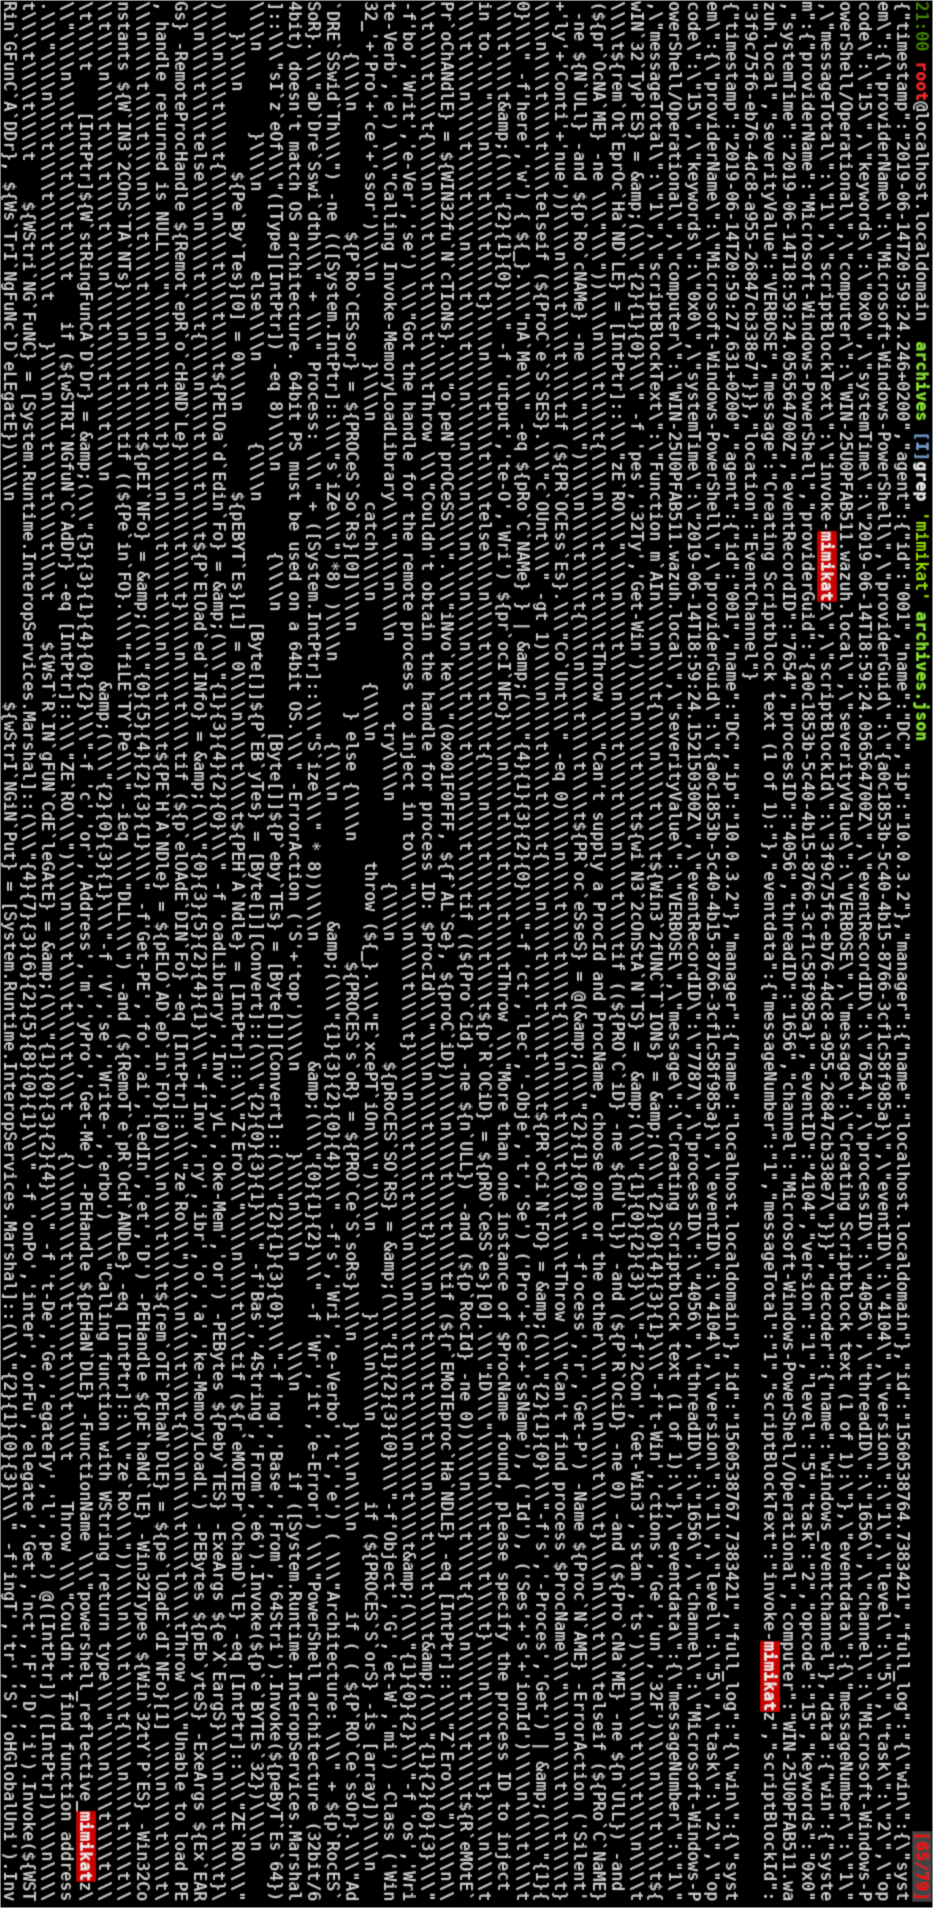
\includegraphics[height=\textheight]{figuras/PSATTACK_mimikatz_rotated.png}
	\caption{Part of PSAttack events in the archives log}
\end{figure}

\subsection{Conclusion}
PowerShell can be very dangerous for the security of Windows systems: it can do almost anything and it has multiple ways to avoid being detected.
These include encoding, encryption, reflective DLL loading and bypassing locks on executables.
All of them have been shown in this project, along with mitigations and/or detection techniques.
\linej
In this section we have only scratched the surface of PowerShell auditing. It would be interesting to have more time for this topic.

\section{Detection of suspicious logins}
In Windows there are multiple ways to login remotely, but all of them rely on the same authentication method. Depending on its success or failure certain security events are issued. Therefore it does not make sense to have multiple ways to reproduce these attacks, as with the previous cases.
\linej
In all these cases the code is run on the no-DC, which authenticates against the DC, using the builtin command \textit{winrs}\cite{winrs}. Here this command is used to specify the remote computer to log in, the user, the password and the command to run after a successful authentication, in that order.
\linej
\linej
Usually this would use a dictionary of common passwords to be mixed with other characters, depending on the password requirements of the AD.
To simplify its emulation, the same passwords will tried all the time.
\linej
\linej
In this section the essential non-functional requirements RNF-03, RNF-04 and RNF-05 are covered.

\subsection{Reverse brute force login attempts} \label{reverse_login}
In this case the attacker tries to login guessing the password without changing his ip address.
He hopes that this goes on undetected because the logins are against different accounts.
\linej
This can be reproduced with a very simple loop:
\lstinputlisting[style=PS]{src/reverse_logins_winrs.ps1}
\linej
Fortunately Wazuh already has rules for this in \textit{0580-win-security\_rules.xml}\cite{wazuh_ruleset}.
Failed logins are identified by the rule 60104, which is triggered by the security event 4771\cite{windows_events}.
Grouping is used by the rule 60205 to trigger another alert with a higher level, if there are at least 8 in 240 seconds from the same ip address.
The value of the MS\_FREQ variable is set to 8 in this file.
\linej
\lstinputlisting[style=xml,captionpos=b,caption=Rule 60205 of Wazuh]{src/rule_60205.xml}

\subsection{Distributed brute force login attempts}
Instead of changing the user the attacker changes his ip address every few attempts. In this case is not so much a matter of not being detected, but of not getting temporary banned by ip address, which usually results in a drop of received packages by the firewall of the network.
\linej
\linej
Usually the attacker would connect from outside of the network, because once inside it would be hundreds of orders of magnitude faster to crack them from a file with credentials.
Instead of changing the ip address of the interface he would change where his remote command comes from, usually using a Virtual Private Network paid service, an anonymity network or previously compromised victims.
Both cases provide multiple servers across the world and is trivial to write a shell command to jump from one to the next.
\linej
The example script \ref{lst:distributed_logins_winrs}\ is mostly about automation to change the ip address for the internal network, which has the interface connected to the \textit{wazuh.local} domain.
Administrator privileges were required to change the ip address successfully. The sleep was found to be an effective measure to avoid trying to log in before the domain was reconnected.
\linej
\linej
The rule 60205 in Wazuh only works for failed attempts comming from the same ip address, therefore it fails to detect this. A similar rule can solve this, just by checking the same user is targeted and by changing the \textit{same\_field} requirement to \textit{not\_same\_field} for the ip address:
\begin{lstlisting}[style=xml]
<rule id="110001" level="3" frequency="5" timeframe="300">
	<if_matched_sid>60104</if_matched_sid>
	<not_same_field>win.eventdata.ipAddress</not_same_field>
	<same_field>win.eventdata.targetUserName</same_field>
	<description>Multiple Windows audit failure events with different IPs</description>
	<options>no_full_log</options>
	<group>pci_dss_10.6.1,gdpr_IV_35.7.d,</group>
</rule>
\end{lstlisting}
\linej
This frequency is fine for testing in a laboratory with an internal network, but probably is way too low for a real environment.
Wazuh can be used to ban the ip for a time with its active response feature\cite{active_response}.

\subsection{Login outside of usual hours}
Allowed logon hours can be set with AD, resulting in failure even with correct passwords when outside of the time range.
Even so we can not rely always in it and there are situations where is interesting to monitor if there are attemps to log in on unusual hours.
For example an attacker would want to breach the network when there is a lesser chance of being detected, for example when the security staff is asleep.
In this case we take interest in detecting these events for users of a certain Organizational Unit, which are useful for AD management.
\linej
\linej
Doing this purely with OSSEC rules would need some hacks to change the code of the rules and restart the manager, for every time the users in the OU change.
Because this changes are possible and because the security events do not report if the user belongs to an OU, we can consider these rules to be like variables.
A workaround would be to name the users with a part of the name of the OU, like \textit{OU1\_user1}, and then have rules matching any username starting with it.
\linej
\linej
Of course these are not acceptable and there is a better way.
Running a remote command with Wazuh we can search the security log for the events of interest, check the hour and verify if they belong to a user of the OU.
As with the klist detection (page \pageref{klist_detection}) a PowerShell script was created \ref{lst:OU}\ and a remote command was set \ref{lst:OU_wodle}.
The script returns JSON output with basic information about the events that met the requirements.
It needs to be run as Administrator to be able to query the security log and it only needs to be in the DCs, since OU logins are made always against them.
The OU name and the hour range are set in the script by hand, but could also be automated.
\linej
\linej
The first part of the script gets the usernames for the OU in question into an array.
\linej
The second is a function that parses the event properties, checking if the conditions are met: the hour of the event is not in the valid range (in this case [8, 17]) and the username is in the previous array.
Next the properties \textit{TargetUserName}, \textit{TimeGenerated}, \textit{OrganizationalUnit} and \textit{EventID} are set in a JSON manner.
The full string is returned at the end of the function, each event in a line.
\linej
The last part is about collecting the security events of interest in the last minutes and calling the function with them. In this case a 10 minute margin was set, because it takes about 5 seconds to query the log each time. The remote command was set to run every 10 minutes to match it.
\linej
We take interest in the event id 4771 for the failures and in the events 4768 (TGT request) and 4769 (TGS request) for the successes\cite{windows_events}.
\linej
\linej
The rules \ref{lst:OU_rules}\ in Wazuh are very simple, the first filters the events that match the format and the second just triggers for everything with an username (since the checks are done in the script).

\subsection{Conclusion}
These login events are very easy to perform, but also to detect.
More sofisticated methods can be used, but is important to remember that brute force logins are not efficient when compared to offline cracking.
There is always a risk of users having unsecure passwords, which can be reduced by enforcing and teaching good password policies.
\linej
Detecting logins in unusual hours can be hard just with OSSEC rules, but it can be solved with a remote script.
\linej
\linej
Again the advantage of using an HIDS is we don't need to monitor every mean of authentication, just 3 events are enough. Combined with the already existing rules and possibilities of remote scripts, Wazuh probes to be a useful tool for management of login events. Other checks could be easily implemented, for example logins from certain ip ranges can be monitored with regular expressions for the ip field (\textit{win.eventdata.ipAddress}).


\cleardoublepage
\chapter{Increment 3}
This increment is titled ``\IncrementoTres''.
It includes an introduction to ransomware, study on simplified and real ransomware and measures against it.
\linej
\linej
In this increment we assume the malware has already breached into the system and our role is to detect and mitigate it, as soon as it begins to hold hostage the system or data.
It does not make sense for this project to study intrusion strategies related to ransomware, because there are too many and there is no guarantee they can be detected by an IDS.

\section{The basics of ransomware}
Ransomware is a term used to describe a class of malware that is used to digitally extort victims into payment of a specific fee.
Is not limited to any particular geography or operating system, and can take action on any number of devices\cite{ransomware_oReilly}.
\linej
Once the ransom is paid the attacker provides the instructions to restore the affected resources.
The best guarantee the ransom works is because attackers are interested in keeping the pay rate as high as possible, but as an illegal activity there is no way to ensure is going to free the system and that it will not be affected again in the future (the attacker could install a backdoor).
\linej
\linej
Any fully functional ransomware needs\cite{ransomware_digital_extortion}:
\begin{itemize}
\item Some mean to hold a resource hostage.
\item An anonymous system for exchanging data with the affected system.
\item A ransom payment method that can not be traced back to the digital extortionist.
\end{itemize}
\linej
There are two basic forms of ransomware, that are not mutually exclusive\cite{ransomware_oReilly}\cite{ransomware_digital_extortion}:
\begin{itemize}
\item Cryto: They encrypt, obfuscate, or deny access to files.
Depending on the target it may search for specific directories or file extensions.
In most scenarios the ransomware does not affect the critical system files or functionalities and does not deny access to the system.
Normally is more sophisticated and targets systems with more robust security than locker ransomware.
\item Locker: They restrict access or lock users out of the system.
Usually the affected system is not able to perform basic tasks, even for payment, which results in a preference of payment voucher systems.
Is easy to recover from but also to implement.
\end{itemize}
\linej
Both can take extra steps, like exfiltrating data or take down any antimalware detected software.
Infected systems are often used by attackers to spread the malware, for example across the network.
The cybercriminal wants the victim to notice as soon as the attack is done, to get paid as fast as possible, and the most common method is sending direct messages or changing the desktop background.
\linej
\linej
The next image shows a simplification of the steps of a ransomware attack.
We only care for the detection of the ``Destruction'' segment, but that does not mean we can ignore the whole picture.
\begin{figure}[H]
	\centering
	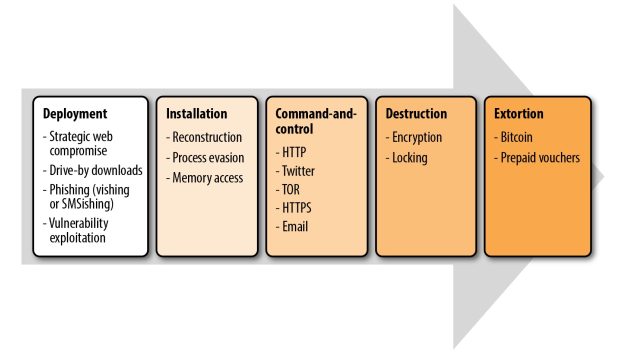
\includegraphics[width=\textwidth]{figuras/anatomy_of_a_ransomware_attack.png}
	\caption{Anatomy of a ransomware attack\cite{ransomware_oReilly}}
\end{figure}

\subsection{State of ransomware}
Ransomware is important for this project because it has gained much relevance in cybersecurity in the last years.
We think understanding it better is the first step to develop detection for it.
\linej
\linej
The main problems for studying ransomware is that is illegal and sometimes is hard to gather information.
For example most of the attacks are not reported and ransomware attacks are often analyzed offline and using auditing tools like decompilers because most of the time there is no source code\cite{ransomware_digital_extortion}.

\subsubsection{The growth of ransomware}
Next there are some estimations about the ransomware economy\cite{ransomware_economy}:
\begin{itemize}
	\item There are more than 6000 dark web marketplaces selling ransomware, with 45000 products listed.
	\item The ransomware marketplace on the dark web has grown in 2502\% from 2016 to 2017.
A major antimalware company states a 90\% increase in detection for business and a 93\% for individuals, in the same year\cite{ransomware_malwarebytes}.
	\item Some sellers of ransomware are making more than 100 thousand USD per year, just by retailing ransomware, when a legitimate software developer makes 30\% less.
\end{itemize}
\linej
Often ransomware includes remote control software to allow the remote execution of commands.
They often check if the server (certain ips or domains) can be reach before starting the process, waiting for a possible connection in the future if not.
Because these domain addresses are always resolving to new host ips, the criminal enterprises can regularly move around the Internet in relative safety, as they will always know their malcode can speak to them.
Keeping this Command and control server functional and anonymous may be hard and expensive depending on the approach used by the attacker.
They have evolved to use algorithms to generate a list of thousands of domains dynamically.
%Particularly DNS scans for new suspicious entries is advised.
\linej
The flaw of this approach is that can trigger behavioural alerts and reduces the scope of the attacks.
There is no need to initially contact the Command and control server, even for crypto ransomware because the public RSA key can be downloaded with the malware.
In some cases the attacker can command the malware to delete itself to avoid leaving evidence for security proffesionals\cite{ransomware_oReilly}\cite{ransomware_digital_extortion}.
\linej
\linej
The fundamental reason why this market exists is because the victims are willing to pay.
Is hard to know specifics because is estimated that most of the times these attacks are not reported (fewer are prosecuted and fewer are sentenced), but the mean crypto ransom is 300 USD per computer\cite{ransomware_digital_extortion}.
\linej
\linej
Unlike many other forms of cyberattacks, ransomware can be quickly and brainlessly deployed with a high probability of profit nowadays.
It has been a revelant type of malware since its beginning 23 years ago, but in the last years its economy has grown hugely, mainly because\cite{ransomware_digital_extortion}\cite{ransomware_economy}:
\begin{itemize}
	\item Bitcoin and Tor: for pseudo-anonymous activities.
	\item Proliferation of service providers: anyone can get into the ransomware business because technical knowledge is not needed for every step of the process.
	\item Lack of fundamental security controls: such as backups, penetration testing, patching, etc.
\end{itemize}
\linej
Bitcoin allows money to be transferred in a way that makes it nearly impossible for law enforcement to follow the money trail.
Anyone can set up a free and unrestricted Bitcoin wallet address without needing any approval from financial institution, regulations, or dealing with providing evidence and proofs of identity, taxation, evidence of residence, and so on.
Anybody can see the Bitcoin transactions or the flow of the cryptocurrency from address to address in the blockchain, making it possible to backtrack it to a real identity.
Unfortunately cybercriminals use to mix transactions to make them very hard to follow, this is what Bitcoin mixing services are for.
\linej
Tor is an anonymity network, that can be used to mask illicit activities and can be used just by running a program.
\linej
Neither provides perfect anonymity, but both are very easy to use, which has lowered the risk and barrier to entry for ransomware perpetrators.
The requirement for ransoms to be paid over the Tor network has ensured there is no centralized endpoint to investigate with traditional geo-based law enforcement approaches\cite{ransomware_digital_extortion}.
\linej
\linej
Due to these innovations, the underground ransomware economy is now an industry that resembles commercial software. It can be divided into sections like: development, support, distribution and even help desks. This market can be divided into tiers\cite{ransomware_economy}:
\begin{itemize}
	\item Authors: They can be responsible for the creation of the malware (including frameworks) and training and support on them. In the current state of the market they can just remain as authors, without ever running the malware in other computers. The cost is based on how customized the code is for a particular target.
	\item RaaS: Ransomware-as-a-Service borrows from the Software-as-a-Service model. RaaS is designed to make ransomware available to even novice criminals. It provides technical and step-by-step information on how to launch the ransomware attack with the purchased software. The most sofisticated have a platform for checking the current status of the attack. In some cases the ransom is split among the members of the supply chain.
	\item Distributors: A high profit/risk tier. They can distribute it themselves by spam campaigns, social engineering, targeted hacks or exploit kits. They can also leverage RaaS.
\end{itemize}
\linej
Splitting the work into different modules makes the ransomware market more complex and competitive.
It encourages role specialization (increasing quality and reducing risk for authors), it makes it easier to enter (expanding the market) and the modularity increases the quantity of different products (making the malware change faster).
\linej
Of course making it easier to enter the market is a double edge sword, because it makes it easier for police to investigate.
Defenders have the inherent advantage of interrupting the entire attack if they can break or interrupt any link of the chain.
\linej
This market can be simplified into the next image:
\begin{figure}[H]
	\centering
	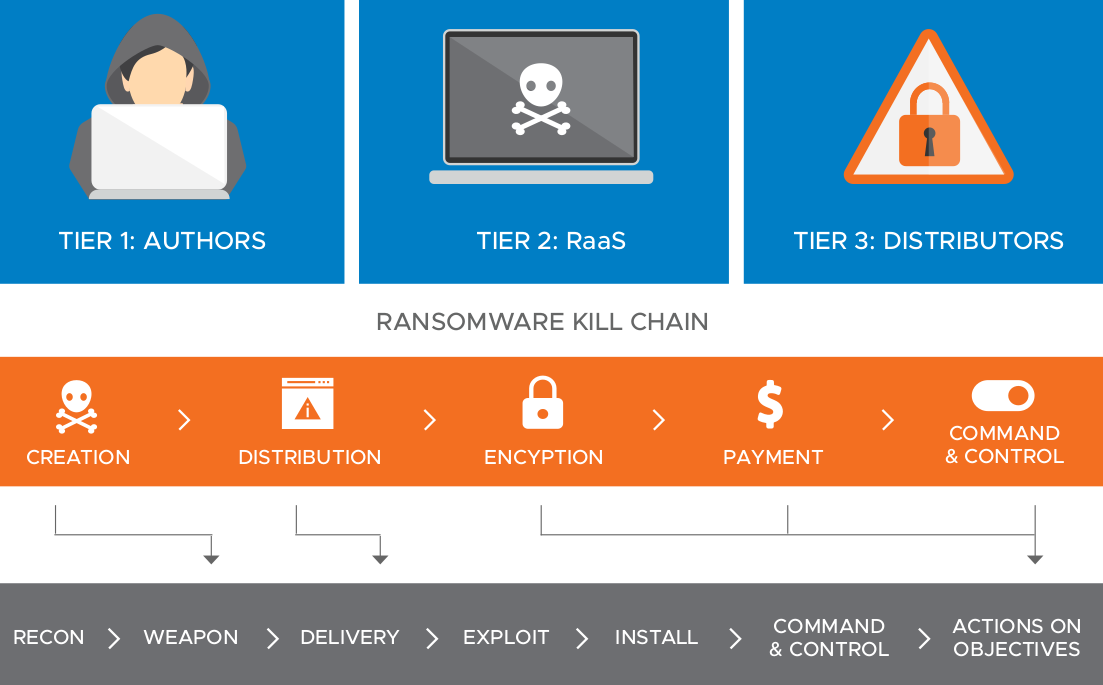
\includegraphics[width=\textwidth]{figuras/ransomware_chain.png}
	\caption{Ransomware supply chain and economy tiers\cite{ransomware_economy}}
\end{figure}
\linej
As long as the victims keep paying the ransom this trend will continue and the specialization will increase, resulting in more and bigger ransomware incidents.
%More creative forms of ransomware are sure to emerge over the years, like encrypting the master boot record\cite{ransomware_digital_extortion}.
The more ransomware is used the more secure the systems are against it, therefore in the future is also safe to assume that it would be more economical for criminals to use cryptominers or credential stealing instead\cite{ransomware_malwarebytes}.
\linej
\linej
Is also interesting to consider how ransomware and other attacks may take place if the main attack fails.
For example even if a ransomware attack fails it should be possible to use a distributed denial of service attack at greater cost and with lesser benefit.
A increase of malware as a distraction is expected in the future as the use and security of backups improves\cite{ransomware_economy}.

\subsubsection{Ransomware targets}
The more important the data the more money the victim is asked for.
Generally the bigger the business the better security it has and the more money cybercriminals can extort.
\linej
But the value of data may change from person to person, therefore there is no absolute best target for ransomware.
In the last years there has been an increase on the number of personal data sold in the dark web, which includes all kinds of data.
Cybercriminals can put pressure on the victim not only with direct ransom but also with the threat of selling the data.
\linej
In practice certain type of targets seems to rate higher on cybercriminals' priority lists\cite{ransomware_digital_extortion}:
\begin{enumerate}
	\item \textbf{Healthcare}: Apparently nothing sells as good on the black market as private healthcare records.
		Medical records do not lose value over time and they contain not only the person's medical history, but offers a full set of sensitive data that can be exploited in more ways than one (credit card numbers, social security numbers, banking credentials, e-mail IDs and employment history).
Cybercriminals use this currency to spread infections by phishing attacks, data fraud, and theft of medical histories.
	\item \textbf{Manufacturing}: Including businesses like automotive, electronics, textile and pharmacy.
The nature of the chemical and automotive businesses makes certain aspects horrifying, however, cybercriminals' motivation is predominantly financial, as they attack corporations not with the intention of mass murder, but to obtain valuable data and lucrative sensitive information.
	\item \textbf{Financial services}: The accessibility of payment methods and globally spread banking services whose main purpose is customer convenience will keep the financial industry high on the list. Attackers only need to impersonate or trick the victim in order to gain access to an account.
	\item \textbf{Goverment agencies}: They hold all types of personal and confidential data. If a goverment agency stops working it can affect many people.
	\item \textbf{Transportation}: Usually ransomware attacks set a time limit to pay the ransom, but in transportation real life sets the time limit. A higher effortless pressure results in less advance malware needs, meaning that transportation businesses could be effectively extorted with locker ransomware or denial of service attacks.
As in previous cases there is also interest in personal data and financial accounts.
	\item \textbf{Home users}: Ransomware is one of the best effective malware against personal computing users, who are considerably not experienced in cybersecurity.
This has increased due to the rise of smartphones and IoT devices.
Most users either don't use backups, they are not done often enough or they are stored in the same computer.
\end{enumerate}
\linej
In the end the target is always the people and the cybercriminal can either create a situation where is cheaper to pay or to gamble on the feelings (fear, shame, guilt, etc) of the victim.
\begin{figure}[H]
	\centering
	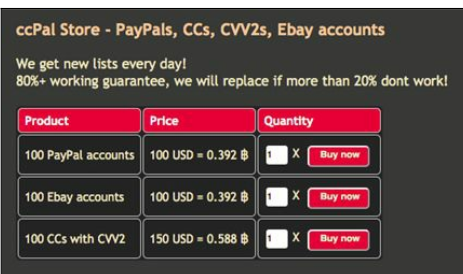
\includegraphics[width=.7\textwidth]{figuras/credit_cards_for_sale.png}
	\caption{Credit cards for sale\cite{ransomware_digital_extortion}}
\end{figure}

\section{Common patterns in crypto ransomware}
64\% of ransomware detected in 2016 was crypto ransomware\cite{ransomware_digital_extortion}, but it was not until 2013 that cybercriminals came back to it as their primary source of ransomware income\cite{ransomware_oReilly}.
The are many different crypto ransomware products, but we take interest in those who encrypt the files because, they are the ones that make the most impact on them.
If the encryption is done with strong algorithms it should not be possible to decrypt them in a lifetime (without knowing the decryption key).
\linej
\linej
This means suspicious activity regarding backups and files is common among the different crypto ransomware variants.
We assume the attacker prefers to execute the attack as fast as possible because:
\begin{itemize}
\item Once the encryption process starts is probably going to be detected very fast, either by an user or by an antimalware detector.
\item The only advantage of waiting is keeping the noise down.
\item If the encryption is only done on key files it should be very fast.
\item The system can be scanned quite silently before starting the encryption.
\end{itemize}
\linej
The most eficient way to encrypt the files is to use a symmetric algorithm (like AES-256), ensuring very strong and fast encryption even for big files.
The symmetric key is the same for encryption and decryption, and in this type of attack it holds the entire value of the ransom: once the ransom is paid the symmetric key is send to the victim to decrypt the files.
\linej
Obviously this key has to be kept secret by the attacker, therefore is ciphered with a public-key asymmetric algorithm (like RSA), allowing the attacker to transfer it without any risk.
Only the people with the private key should be able to decipher the symmetric key, therefore only the attacker can decipher it.
The public key is either downloaded with the malware or after the installation.
\linej
A major disadvantage of symmetric key encryption is that, in some cases, the key can be retrievered from RAM using special software.
Fortunately the DRAM in most systems is still live for anywhere from a few seconds to a few minutes after power loss, allowing a shutdown to stop the attack and still being able to recover from it.
However these techniques are unlikely to work with functions that avoid leaving trails in memory\cite{ransomware_oReilly}.
\linej
\linej
Most ransomware families use the built-in Windows Crypto API to handle the encryption.
While this is not a process that can necessarily be blocked, it is a process on which a security team can be alerted.
The problem is not detecting its use, but rather not spawning false positives\cite{ransomware_oReilly}.
\linej
\linej
Because the attack is supposed to be fast, the detection (and response) needs to be even faster to be able to stop it.
That is why multiple detection ways were explored for this case of study:
\begin{itemize}
\item For file encryption:
	\begin{itemize}
		\item Windows Defender's Controlled Folder Access
		\item Sysmon events
		\item Windows File Auditing
		\item Syscheck Monitoring with Wazuh
	\end{itemize}
\item For backup deletion:
	\begin{itemize}
		\item Detection of certain commands
		\item Increase of the backup volume free storage space
	\end{itemize}
\end{itemize}

\subsection{File encryption example}
This example shows how easily removal and encryption of files can be done with the right tools.
\linej
In this scenario the attacker uses AES for the files and ciphers the key passphrase with a RSA public key.
Both algorithms are supported by many tools: GnuGG, OpenSSL, custom DLLs and programming languages like PowerShell or Python.
OpenSSL was chosen because it works the same on Windows and GNU/Linux and is easy to use and install.
\linej
\linej
The first step would be the generation of the pair of RSA keys.
The private key stays in the computer of the attacker and the public key is stored into the victim's.
In this case the files are named ``keys.pem'' and ``public.pem'' respectively and the length of the key is 1024 bits.
The first file includes both private and public keys.
The second file is generated by the second command, which extracts the public key out of the combined file ``keys.pem''.
\begin{lstlisting}[style=PS,keywordstyle=\color{black}]
openssl genrsa -out keys.pem 1024
openssl rsa -in keys.pem -pubout -out public.pem
\end{lstlisting}
\linej
The next PowerShell script creates a random passphrase of letters, numbers and some special characters, which is used later for the symmetric key by the AES implementation of OpenSSL.
This passphrase is ciphered with the public RSA key and saved to the file ``passphrase.txt''.
Then script loops over all the files in \textit{C:/temp/} with the \textit{.txt} extension, encrypting them to AES-256 (in block cipher mode) and deleting the original file when done.
The \textit{openssl} variable is just for convenience.
\lstinputlisting[style=PS,caption=Script to encrypt files and cipher the passphrase with RSA,captionpos=b,label={lst:ransomware_basic}]{src/ransomware_basic.ps1}
\linej
The passphrase file can be deciphered with the private key, getting the random passphrase used in the script:
\begin{lstlisting}[style=PS,keywordstyle=\color{black}]
openssl rsautl -decrypt -in passphrase.txt -inkey keys.pem
\end{lstlisting}
\linej
Decrypting the files can be done using the same passphrase, because AES is a symmetric algorithm.
This example assumes the same value for the variables as in the encryption process:
\lstinputlisting[style=PS]{src/ransomware_decrypt.ps1}

\subsection{Detection of file crypto ransomware}
Next some sources for possible detection of crypto ransomware are examined.
Each of these options has its pros and cons, there is no restriction for using them toguether (in case one fails).
It is important to keep in mind that the Wazuh server is supposed to manage multiple systems, therefore scalability should be a concern and maybe only one of the solutions could be used in a real network.

\subsubsection{Windows Defender's Controlled Folder Access}
Windows Defender has the option to monitor specified folders for accesses and/or modification on real-time.
This feature is designed to combat the threat of ransomware.
It includes the option to whitelist applications and two basic modes of operation\cite{hardening_windows_10}:
\begin{itemize}
	\item Audit: Just notifies about suspicious activity with the event 1124.
	\item Block: Blocks and notifies about suspicious activity with the event 1123.
\end{itemize}
\linej
These events trigger for any suspicious activity, not only for ransomware attacks, but their detection is trivial \ref{lst:windows_defender}.
Windows Defender event log can be forwarded to Wazuh \ref{lst:forward_Windows_Defender}, allowing to improve the protection provided by Windows Defender with Wazuh.
The configuration of the whitelisted applications and the monitored directories can be managed by the Group Policy, the Windows Defender interface or the registry.
\linej
Windows defender has a set of monitored folders by default and the rest are listed in \textit{Computer{\textbackslash}HKEY\_LOCAL\_MACHINE{\textbackslash}SOFTWARE{\textbackslash}Policies{\textbackslash}Microsoft{\textbackslash}Win- dows Defender{\textbackslash}Windows Defender Exploit Guard{\textbackslash}Controlled Folder Access{\textbackslash}Pro- tectedFolders}.

\subsubsection{Sysmon events for file changes}
Sysmon events can be used to monitor changes in folders too, for example monitoring the folder \textit{C:{\textbackslash}temp{\textbackslash}}:
\begin{lstlisting}[style=xml]
<!--EVENT 2: FILE CREATION TIME RETROACTIVELY CHANGED IN THE FILESYSTEM-->
<FileCreateTime onmatch="include">
	<TargetFilename condition="contains">C:\temp\</TargetFilename>
</FileCreateTime>

<!--EVENT 9: RAW DISK ACCESS-->
<RawAccessRead onmatch="include">
	<Device condition="contains">C:\temp\</Device>
</RawAccessRead>

<!--EVENT 11: FILE CREATED-->
<FileCreate onmatch="include">
	<TargetFilename condition="contains">C:\temp\</TargetFilename>
</FileCreate>
\end{lstlisting}
\linej
Unfortunately none of the Sysmon events can detect file deletion, but they can be useful in other ways:
\begin{itemize}
	\item Event 2 could detect backdoors, which would change some key file and restore its previous creation time. Is not uncommon for ransomware to install them to extort the system in the future. Instead of relying on this event is a safer idea to use file integrity monitoring, checking the checksum of each key file for changes.
	\item Event 9 can be used to detect direct reading of the device, an alternative access method to avoid being detected by traditional file monitoring, like in the case of NinjaCopy \ref{invoke-NinjaCopy}.
	\item Event 11 can detect the new files, which could be identified as encrypted files in some cases with active response. Depending on the directory and the Wazuh rules there may be false positives.
\end{itemize}
%\linej
%For the execution of this example (with 4 .txt files) Windows Defender reported 6 events of type 1124 and Sysmon 5 of type 11 (4 creations of .txt.enc and symmetric.key).
%This makes sense because events 2 and 9 are triggered by change of creation time and raw access of the drive respectively.
%It is important to note that if the changes are blocked only events of type 1123 are generated.

\subsubsection{Windows File Auditing}
Windows File Auditing is a security feature that can be enabled and configured for multiple folders, reporting with events [4656-4663].
\linej
Windows does not log file activity in an usual way.
Instead, it logs granular file operations that require further processing and they are usually out of order.
The next table tries to describe and show the difference between these events as simple as possible\cite{windows_events}\cite{events_46_56_X}:
%\begin{table}[H]
	%\begin{tabularx}{\textwidth}{|l|X|X|}
		%\hline
		%\rowcolor{gray!30}
		%Event ID & Name and description & Useful data\\ \hline
		%4656& A handle to an object was requested. Logs the start of every file activity but does not guarantee that it succeeded.&
			%$\bullet$ Executable responsible
			%\linej $\bullet$ Filename of the object
			%\linej $\bullet$ Access mask
			%\linej $\bullet$ Accesses
			%\\ \hline
		%4658& The handle to an object was closed. Logs the end of a file activity.&
			%$\bullet$ Executable responsible
			%\\ \hline
		%4659& A handle to an object was requested with intent to delete. Logs a failed attempt to delete.&
			%$\bullet$ Executable responsible
			%\linej $\bullet$ Access mask
			%\\ \hline
		%4660& An object was deleted. Logs a delete operation.&
			%$\bullet$ Executable responsible
			%\\ \hline
		%4663& An attempt was made to access an object. Logs the specific micro operations performed as part of the activity.&
			%$\bullet$ Executable responsible
			%\linej $\bullet$ Filename of the object
			%\linej $\bullet$ Access mask
			%\linej $\bullet$ Accesses
			%\\ \hline
	%\end{tabularx}
	%\caption{Windows File Auditing events}
%\end{table}
\begin{table}[H]
	\begin{tabularx}{\textwidth}{|l|X|}
		\hline
		\rowcolor{gray!30}
		Event ID & Name and description\\ \hline
		4656& A handle to an object was requested. Logs the start of every file activity but does not guarantee that it succeeded.\\ \hline
		4658& The handle to an object was closed. Logs the end of a file activity.\\ \hline
		4659& A handle to an object was requested with intent to delete. Logs a failed attempt to delete.\\ \hline
		4660& An object was deleted. Logs a delete operation.\\ \hline
		4663& An attempt was made to access an object. Logs the specific micro operations performed as part of the activity.\\ \hline
	\end{tabularx}
	\caption{Windows File Auditing events}
\end{table}
\linej
More detail and thought is needed to complete the previous table\cite{windows_events}\cite{events_46_56_X}:
\begin{itemize}
	\item If an operation is rejected because not having enough privileges the only event issued is 4656.
	\item Windows only issues the event 4663 when the operation is complete. There might be multiple 4663 events for a single handle, logging smaller operations that make up the overall action.
	\item There are some events that do not appear in the previous range: 4657 is for registry changes and 4661 and 4662 are for AD objects.
	\item Events 4656 and 4663 include the ``accesses'' property, which refers to the type of operation: read, write, delete.
		The field can include multiple values, for example a rename involves read, delete and write.
		The problem of this field is that it does not follow a very normal interpretation of these types of basics operations.
	\begin{itemize}
		\item``WriteData'' implies that a file was created or modified unless a ``delete'' access was recorded for the same handle. The only way to know if it was created or if it was modified is to know if the file existed before, for example with a database.
		\item``ReadData'' is logged almost in every case, resulting in only being a normal read if none of the others are recorded.
		\item``Delete'' also includes move events. Move events do not spawn 4659 or 4660 events.
	\end{itemize}
	\item The path included in the event may be the device path, for example ``{\textbackslash}{\textbackslash}Device{\textbackslash}{\textbackslash}Harddisk- Volume3{\textbackslash}{\textbackslash}openssl{\textbackslash}{\textbackslash}bin{\textbackslash}{\textbackslash}bftest.exe'', instead of the normal volume path like ``c:{\textbackslash}temp''.
\end{itemize}
\linej
We can conclude that these events are not as easy to handle as they could be, but they can still be used for the detection of ransomware.

\subsubsection{Syscheck Monitoring with Wazuh}
Wazuh can check file changes directly checking checksum differences with the Syscheck module, this is known as File Integrity Monitoring.
Each agent maintains its own database for better performance.
\linej
The monitoring needs to be configured \ref{lst:syscheck_agent}\ in the agent, instead of the manager.
This generates Syscheck events that can be processed by rules, triggering alerts.
Syscheck has many options, like files to be ignored (which can also be done with rules) or the maximum recursion level to monitor.
\linej
The most interesting features of Syscheck for this project are\cite{libro_ossec}:
\begin{itemize}
	\item Real-time monitoring. It can only be set at folder level, not directly for files, but that can be worked around with ignores in fixed cases or match restrictions in rules.
	\item Scheduled scan. Interesting from a scalability point of view for checking security settings and looking for rootkits, but not useful for inmediate detection.
	\item Inmediate scan. The agent can be ordered to do a scan at any time. This is interesting to combine with active response.
	\item The creation and deletion of files can be detected too.
\end{itemize}

\subsubsection{Comparison of the different monitoring alternatives}
The previous analysis is interesting but a conclusion is yet to be reached.
Each of the next tables shows a simplification of the advantages and disadvantages of each of the examined methods:
\newcolumntype{w}{>{\hsize=.5\hsize}X}
\begin{table}[H]
	\begin{tabularx}{\textwidth}{|w|w|}
		\hline
		\rowcolor{gray!30}
		Advantages & Disadvantages\\ \hline
			$\bullet$ It allows the accesses to be blocked (in Block mode).
			\linej $\bullet$ It can detect any kind of creation, modification and deletion.
			\linej $\bullet$ False positives are uncommon.
			\linej $\bullet$ Provides abstraction to the end user. Windows decides which programs are legitimate.
			\linej $\bullet$ Legitimate whitelisting. Blacklisting can be implemented with rules in Wazuh.
			\linej $\bullet$ Fundamentally faster active response than Wazuh, which adds multiple steps to the direct response of Windows Defender in block mode.
		&
			$\bullet$ The logs do not include the filename, just the folder path.
			\linej $\bullet$ The logs do not explain the reason to find the event suspicious.
			\linej $\bullet$ The logs do not detail the kind of file event (creation, modification or deletion).
				%During the testing they always reported ``blocked from modifying''.
			\linej $\bullet$ It is an external program, therefore it can not be totally trusted to work on complex cases.
			\linej $\bullet$ It is one of the most and first denfensive programs targeted by attackers.
			\linej $\bullet$ The whitelisting may need manual adjustment, for example allowing the Wazuh agent.
			\\ \hline
	\end{tabularx}
	\caption{Advantages and disadvantages of file monitoring with Windows Defender}
\end{table}

\begin{table}[H]
	\begin{tabularx}{\textwidth}{|w|w|}
		\hline
		\rowcolor{gray!30}
		Advantages & Disadvantages\\ \hline
			$\bullet$ They can detect other malware approaches to the files.
		&
			$\bullet$ They can not be used to detect any kind of changes.
			\linej $\bullet$ Real malware can be hard to tell apart from false positives.
			\\ \hline
	\end{tabularx}
	\caption{Advantages and disadvantages of file monitoring with Sysmon events}
\end{table}

\begin{table}[H]
	\begin{tabularx}{\textwidth}{|w|w|}
		\hline
		\rowcolor{gray!30}
		Advantages & Disadvantages\\ \hline
			$\bullet$ They can be used to detect any kind of creation, modification and deletion.
		&
			$\bullet$ They can be too complex and counterintuitive. Following their flow requires composite rules in Wazuh.
			\linej $\bullet$ Lack of critical information in the logs.
			\linej $\bullet$ Real malware can be hard to tell apart from false positives.
			\\ \hline
	\end{tabularx}
	\caption{Advantages and disadvantages of file monitoring with Windows File Auditing events}
\end{table}

\begin{table}[H]
	\begin{tabularx}{\textwidth}{|w|w|}
		\hline
		\rowcolor{gray!30}
		Advantages & Disadvantages\\ \hline
			$\bullet$ They can be used to detect any kind of creation, modification and deletion.
			\linej $\bullet$ Diff is supported for text files.
			\linej $\bullet$ They always include critical information, like the filename and the program.
		&
			$\bullet$ Real malware can be hard to tell apart from false positives.
			\linej $\bullet$ The format of the events is not suited for field matching.
			\\ \hline
	\end{tabularx}
	\caption{Advantages and disadvantages of file monitoring with Syscheck events}
\end{table}
\linej
From these tables we can conclude that:
\begin{itemize}
	\item Fast local action is more suited to antivirus than IDS, therefore it makes sense to turn to Windows Defender for this feature. Further actions can still be implemented with Wazuh active response. For the others the active response is still possible, but slower.
	\item Windows Defender is the most attractive method to detect and stop the malware, but there are risks in only trusting Windows Defender.
	\item Because is hard to detect the creation of new files with the Windows File Auditing it makes sense to use the event 11 of Sysmon for this and likewise Sysmon can not detect file deletion which this security auditing can. But both have fundamental problems with false positives.
	\item Direct monitoring with Wazuh seems to be easier and more effective that combining Windows File Auditing with Sysmon.
	\item The Sysmon events 2 and 9 are always useful to find suspicious events with a low chance of false positives.
	\item Windows Defender detects the attack on its own, while the others need to relate multiple events in a short period of time with Wazuh's composite rules.
\end{itemize}

\subsubsection{Protecting Windows Defender}
If Windows Defender is chosen for protection against ransomware then it makes sense to improve the protection of Windows Defender because is very targeted by attackers.
This project can not afford much time on this task, but it can provide a solution for the most basic way to deactivate Windows Defender completely or just any of the features against ransomware.
The easiest way for an attacker to do this is to use the Windows registry, therefore enabling or disabling directly the functionality in question.
\linej
Access to the registry can be hardened, but in this case is assumed that not allowing to use access to registry editing tools is not enough to prevent an skilled attacker from doing so.
\linej
In the end this is a complex problem that does not only affect Windows Defender (the Wazuh agent is a similar case) and is impossible to fully solve, but measures can be taken nonetheless.
\linej
\linej
There may exist better ways to ``block'' registry changes, but none were found.
The objective is to assure that certain entries never are set to 1 and that other entries are always set to 1.
In the registry the value 1 often means the setting is enabled.
In this scenario we assume the system has the entries with the desired values from the beginning.
\linej
More specifically the entries to avoid being 1 are in \textit{HKLM{\textbackslash}SOFTWARE{\textbackslash}Policies {\textbackslash}Microsoft{\textbackslash}Windows Defender{\textbackslash}}:
\begin{lstlisting}[style=xml,frame=none]
	Spynet\SpyNetReporting
	DisableAntiSpyware
	DisableBehaviorMonitoring
	DisableOnAccessProtection
	DisableScanOnRealtimeEnable
\end{lstlisting}
\linej
And the entries to keep their value as 1 are in \textit{HKLM{\textbackslash}SOFTWARE{\textbackslash}Policies{\textbackslash}Mi- crosoft{\textbackslash}Windows Defender{\textbackslash}Windows Defender Exploit Guard{\textbackslash}Controlled Folder Access{\textbackslash}}:
\begin{lstlisting}[style=xml,frame=none]
	EnableControlledFolderAccess
	ExploitGuard_ControlledFolderAccess_AllowedApplications
	ExploitGuard_ControlledFolderAccess_ProtectedFolders
\end{lstlisting}
\linej
Wazuh can monitor the registry for changes, but not creation, and Windows also has auditing features that allow to monitor the registry, but Sysmon seems easier to configure.
Periodic checks for changes, in case an event report was lost, can easily be done in Wazuh with the remote command feature.
Other real-time checks could also be implemented, like ensuring the Windows Defender process is running as expected.
\linej
Monitoring the registry for creation/deletion, value changes and renaming can be done with Sysmon events [12-14] respectively.
In this case we only need to monitor a few entries \ref{lst:sysmon_events_registry}.
These events can be a bit odd:
\begin{itemize}
	\item The Windows registry can use a temporary name for an entry, at least when manually creating one with the graphical user interface.
	\item There is no need to change the value in order to spawn an event 13, the execution of a change command is enough.
	\item An entry can be created with the desired value directly, only spawning an event 13.
	\item In the case of renaming there may not be an event of id 14, but one of id 13 (with the old name) followed with an event of id 12 (with the new name).
\end{itemize}
\linej
This means that the easies way to manage them is to:
\begin{itemize}
	\item Delete or set to 0 the entries to avoid being 1. This should be triggered by any of the [12-14] events, except the event 13 when the value is set to 0 (to avoid recursion).
	\item Create and set to 1 the entries that always should be 1. It should only happen when the entry is deleted or renamed.
	\item Set to 1 the entries that always should be 1. It should only happen when the entry is changed.
\end{itemize}
\linej
The rules to accomplish this are very simple \ref{lst:rules_registry}.
The only detail that can lead to confussion is the use of the \textit{field} tag to filter the event id instead of using the \textit{if\_group} tag, which is because \textit{if\_sid} with \textit{if\_group} interact as a logical OR, but \textit{if\_sid} with \textit{field} interact as a logical AND.
\linej
These rules cover the previous cases toguether with the active response configuration \ref{lst:active_response_registry}.
\linej
\linej
The active response command is executed on the agent that triggered the alert, running a CMD script, which runs a PowerShell script.
Direct execution of PowerShell is not possible yet, but it is in the works.
This is documented from \ref{lst:change-registry-value_0}\ to \ref{lst:delete-registry}.
For undesired entries changing the value and the deletion can both be used.
%The first time the active response was enabled the deletion did not work because a lack of privileges, which should be solved with:
%\begin{lstlisting}[style=PS]
%icacls 'C:\Program Files (x86)\ossec-agent\active-response\bin\change-registry-value_0.cmd' /setowner SYSTEM
%\end{lstlisting}
%Oddly enough after a reboot it started to work, even without setting the owner to SYSTEM.
\linej
\linej
In this case the entries were grouped for both rules and active response scripts, therefore instead of executing the command for only the affected entry it is done for the whole group.
This could be solved in multiple ways:
\begin{itemize}
	\item Having an alert and active response command for each entry.
	\item Sending the affected entry name as an argument. This can not be done yet in Wazuh.
	\item Having the final PowerShell script check manually the status to only work on the affected entry.
\end{itemize}
\linej
None were implemented because there is no downside at this scale to just execute script for all the related entries.
The main problem with this approach is the management is harder than if it were centralized.
%https://github.com/wazuh/wazuh-ruleset/issues/155
	%3002 - Real time protection encountered an error and failed.
	%5001 - Real time protection is disabled
	%5004 - Real time configuration changed
	%5007 - The antimalware platform configuration changed
	%5010 - Scanning for malware and other potentially unwanted software is disabled.
	%5012 - Scanning for viruses is disabled.
	%5101 - The antimalware platform is expired

\subsubsection{Reducing false positives}
In this case the problem with detection methods other than Windows Defender's Controlled Folder Access is there is no guarantee that the reported events are from normal and legitimate operations.
There are many circumstancial solutions like: maintaining a list of allowed applications or looking for suspicious behaviour (for example many files created and later deleted in a short time).
But none of them are guaranteed to always work by default.
Instead a simpler approach was implemented: use decoys and look for suspicious behaviour.
Because Windows Defender does not provide the filename decoy filtering can not be used with it.
\linej
The deletion of files was chosen as the suspicious behaviour to detect, because there is no need to save the encrypted files in the same directory.
Mass creation of files can also be detected and identified as suspicious.
\linej
\linej
Decoy files are files that appear to be normal files but should never be changed or deleted by a legitimate user.
Therefore if there are such events paired with other suspicious behaviour in a short amount of time it should mean that a ransomware attack is going on.
\linej
These restrictions can be increased to reduce the chance of generating false positives at the risk of losing real positives.
Increasing the required number of other deleted files over the minimum of two \ref{lst:syscheck_rules_2}, for the decoys and Wazuh composite rules, in contrast with the normal rules \ref{lst:syscheck_rules}.
\linej
There are ways to hide decoy files for normal users and to automate their creation, but that is trivial and not the objective of this section.
To reduce the file storage used by the decoys hard links and soft links could be used, but there is no guarantee that ransomware would treat the files exactly as the rest, therefore reducing the chance of the detection to work.
\linej
In this example the decoys are just named ``decoy1'' and ``decoy2'' for simplification.
Two decoys are used instead of only one with a complex way to duplicate its alert (like using active response), because the storage space should not be affected by this and it is easier.
\linej
\linej
Decoys proved to work on testing with the encrypting script \ref{lst:ransomware_basic}\ and detection with both Windows File Auditing \ref{lst:file_audit}\ and Syscheck Monitoring with Wazuh \ref{lst:syscheck_rules}.

\subsection{Backup deletion}
Backups provide effective mitigation against crypto ransomware attacks in most cases.
There are many scenarios between distributed backups in servers accross the world and just having local backups.
Their ability to overcome ransomware attacks depends on multiple factors like: the exact malware, the distribution of the backup system, the security of the backup system, etc.
\linej
In this case we assume the target only has local backups that are managed with the Shadow Copy service, which allows files to be copied even when in use.
%A Shadow Copy storage can be added to a device and a Shadow Copy can be created as easily as:
%\begin{lstlisting}[style=xml]
%vssadmin add shadowstorage /For=C: /On=F: /MaxSize=50%
%vssadmin create shadow /For=C:
%\end{lstlisting}
%\linej
Some known ransomware like Locky and Cerber try to delete existing Shadow Copies before encrypting the files\cite{ransomware_oReilly}:
\begin{lstlisting}[style=PS]
C:\Windows\system32\vssadmin.exe delete shadows /all /quiet
C:\Windows\system32\wbem\wmic.exe shadowcopy delete
\end{lstlisting}
\linej
Only vssadmin was used for testing because wmic is just the same but from remote (and is even easier to detect because it has three specific Sysmon events).
A new disk was added to the virtual machine of the SMB server to serve as a Shadow Copy storage on the \textit{F:} drive.
This and a network disk are the most basic methods for scheduling backups using Shadow Copies, due to Windows restrictions.
\linej
\linej
It is not possible to detect the deletion of Shadow Copies with file monitoring methods like: Sysmon events, Windows' File Activity Monitoring events and Windows Defender's Controlled Folder Access.
The Shadow Copies are not in the filesystem of the volume, they are managed directly by the Shadow Copy service as special storage.
%TODO detection
%detectar borrado de backups mirando el tamaño libre en el volumen
	%si disminuye se actualiza (CBC database?)
	%si aumenta se debe de haber borrado algo


\subsection{Active response against ransomware}
%TODO


%TODO real ransomware tests
%\section{}
%TODO table detection Yes/No colors
%\begin{table}[H]
	%\centering
	%\begin{tabular}{|l|l|l|}
		%\hline
		%\rowcolor{gray!30}
		%Ransomware variant & Detected \\ \hline
		%TODO& \RYES\\ \hline
	%\end{tabular}
	%\caption{Real ransomware detection by previous methods}
%\end{table}

\section{Mitigation}
Ransomware does not need any particular weakness or vulnerability to work on a system, but the better protected the system is the harder it is for it to be victim of a ransomware attack.
Next are some of the most basics measures to mitigate ransomware attacks\cite{ransomware_oReilly}\cite{ransomware_digital_extortion}\cite{hardening_windows_10}:
\begin{itemize}
	\item Prevent the ransomware from accessing the Windows Registry:
Ransomware can use the registry to maintain persistence through reboots and to disable security features on the victim machine.
Administrators can disable writing to at least to certain registry keys using Windows Resource Protection.
	\item Cyber insurance:
In some cases it may reduce certain costs, like: notifications costs to data breach victims, loses from offline periods, legal defense costs and forensics and investigation costs.
	\item Using decoy resources:
They can be used to detect unplanned acceses or changes and to find vulnerable systems (using honeypots).
	\item Security awareness and education:
It is important to teach the basics of cybersecurity threats to its targets.
For example being careful with web browsing and everyday documents like PDFs or Mircrosoft Office documents, all of which can contain malware that runs on access.
	\item Fundamental security controls:
They provide the base for the cybersecurity of the system.
Their vulnerabilities may allow or increase the scope of all kinds of attacks.
They may change from system to system, but the basic are: backups, penetration testing, patching, software updates, firewall, antimalware software and advanced security options (like Exploit Protection, Secure Boot and Early Launch Antimalware).
	\item Granular permissions and isolation:
Minimizing the available administrator accounts to attackers, by reducing its number and keeping them as isolated as possible, is a good way to mitigate their threat.
For example it makes sense to require administrator privileges for the backup service, which is key for crypto ransomware, even when they are remote backups.
They can mean the difference between compromising just a system or the whole network, when a system becomes a central point of failure.
	\item Restrictions to unnecessary services and software:
They may not be enough to keep the attacker away from using the software, but at least they probably would rise some alerts or slow the process.
In some cases the attacker may reconsider the target to not be worth the effort.
Some of the recommended restrictions are over: Tor, powershell, vssadmin, wmic, certain directories and not digitally signed software.
	\item Removing unused devices:
Basic action to prevent possible further infection spreading.
It should be applied to physical devices like: mapped drives, USB storage devices or memory sticks and smartphones.
All writeable devices should be removed from a station when not in use.
	\item File exchange management:
Many businesses need file sharing to worked on collaboratively.
Once the process of file sharing becomes a routine, security gets on wobbly feet.
To keep the filesystem safe, organizations should establish best practices for sharing data and files in a safe and secure manner.
An effective way to minimize risks is application of digital signatures.
	\item Response plan development:
At a moment of crisis, decision-making can be weak exacerbating the consequences of the infection.
Developing a solid plan for fighting malware infections is the first mitigation task that should be completed by the responsible business leaders in the organization.
\linej
Next is a quick five-step guide for businesses under attack:
	\begin{itemize}
		\item Disabling sync features:
Enabled syncing features makes it easier for offenders to instigate attacks that will overwrite files, especially when they use crypto ransomware.
By disabling sync features you can prevent targeting data in the cloud.
		\item Removing malware from the affected devices:
There are two basic ways to do this: scan the systems or replicate the system from scratch.
The first option is usually faster but there is no 100\% guarantee to detect the malware, while the second needs preparation beforehand (for example with backups) and time with services unavailable.
Replicate the system from scratch can be much more easier and faster with virtualization management.
		\item File recovery:
Depends on the system version in use and there may me data that can not be restored.
		\item Blocking the payment transaction:
Under certain circumstances, the payment transaction can be blocked, even if you have already started the payment process.
This is throughble when the files have been successfully recovered without using the help provided by the attackers.
		\item Contacting law enforcement and reporting the crime:
It is important not only for taking action in the concrete case, but also for predicting and protecting against future cases.
Sending a report to the relevant software authorities is also recommended.
If there were more reports then there would be more data on ransomware attackes, making it easier to defend against it.
	\end{itemize}
\end{itemize}


%\section{Conclusion}
%TODO



\cleardoublepage
\chapter{Conclusions and additions}
\chapter{Conclusions and additions}

%TODO




\appendix
\cleardoublepage
\chapter{Glossary}


%TODO


%\cleardoublepage
%\chapter{Technical Manual}

%Manuais técnicos: en función do tipo de Traballo e metodoloxía empregada, o contido poderase dividir en varios documentos. En todo caso, neles incluirase toda a información precisa para aquelas persoas que se vaian a encargar do desenvolvemento e/ou modificación do Sistema (por exemplo código fonte, recursos necesarios, operacións necesarias para modificacións e probas, posibles problemas, etc.). O código fonte poderase entregar en soporte informático en formatos PDF ou postscript.

%TODO


%\cleardoublepage
%\chapter{User Manual}

%Manuais de usuario: incluirán toda a información precisa para aquelas persoas que utilicen o Sistema: instalación, utilización, configuración, mensaxes de erro, etc. A documentación do usuario debe ser autocontida, é dicir, para o seu entendemento o usuario final non debe precisar da lectura de outro manual técnico.


%TODO


\cleardoublepage
%done="$(\grep -oh 'ref{lst:\w*}' *.tex | cut -d '{' -f2 | tr '\n' '|')"; \grep -oh 'label={lst:\w*}' code-configuration.tex | \grep -vE "${done:0:-1}"

\chapter{Programming and configuration code}
%\lstinputlisting[style=xml,caption=,captionpos=b]{src/}
%\lstinputlisting[style=PS,caption=,captionpos=b]{src/}

\section*{Detection of the use of the TGT with klist}
\lstinputlisting[style=xml,caption=Remote command configuration in \textit{/var/ossec/etc/shared/default/agent.conf} for the klist script,captionpos=b,label={lst:klist_wodle}]{src/klist_wodle.xml}
\linej
\lstinputlisting[style=PS,caption=Script to scan and parse to JSON the tickets in the cache,captionpos=b,label={lst:klist}]{src/klist.ps1}
\linej
\lstinputlisting[style=PS,caption=Way to get the MaxTicketAge from the Group Policy,captionpos=b,label={lst:klist_getMaxTicketAge}]{src/report.ps1}
\linej

\section*{Detection of suspicious logins}
\lstinputlisting[style=PS,caption=Distributed brute force logins changing the ip address for the internal network,captionpos=b,label={lst:distributed_logins_winrs}]{src/distributed_logins_winrs.ps1}
\linej
\lstinputlisting[style=xml,caption=Wazuh rules for checking OU logins outside of usual hours,captionpos=b,label={lst:OU_rules}]{src/rules_OU.xml}
\linej
\lstinputlisting[style=xml,caption=Remote command configuration in \textit{/var/ossec/etc/shared/default/agent.conf} to find logins on unusual hours for the OU users,captionpos=b,label={lst:OU_wodle}]{src/OU_wodle.xml}
\linej
\lstinputlisting[style=PS,caption=Remote script to find logins on unusual hours for the OU users,captionpos=b,label={lst:OU}]{src/OU.ps1}
\linej

\section*{File monitoring}
\lstinputlisting[style=xml,caption=Windows Defender's Controlled Folder Access rules,captionpos=b,label={lst:windows_defender}]{src/rules_windows_defender.xml}
\linej
\lstinputlisting[style=xml,caption=Syscheck local configuration in the \textit{ossec.conf} file on the agent,captionpos=b,label={lst:syscheck_agent}]{src/syscheck_agent.xml}
\linej
\lstinputlisting[style=xml,caption=Syscheck rules for crypto ransomware detection,captionpos=b,label={lst:syscheck_rules}]{src/rules_syscheck.xml}
\linej
\lstinputlisting[style=xml,caption=Syscheck rules for crypto ransomware detection with more deletion events required,captionpos=b,label={lst:syscheck_rules_2}]{src/rules_syscheck_2.xml}
\linej
\lstinputlisting[style=xml,caption=Windows File Auditing rules for crypto ransomware detection,captionpos=b,label={lst:file_audit}]{src/rules_file_audit.xml}
\linej

\lstinputlisting[style=xml,caption=Wazuh rules for detecting encrypted files,captionpos=b,label={lst:trid_rules}]{src/trid/rules_trid.xml}
\linej
\lstinputlisting[style=xml,caption=Active response configuration in \textit{/var/ossec/etc/shared/default/agent.conf} for the Trid CMD,captionpos=b,label={lst:trid_ossec}]{src/trid/ossec.conf}
\linej
\lstinputlisting[style=PS,caption=CMD script only for executing the Trid PowerShell script,captionpos=b,label={lst:trid_cmd}]{src/trid/trid.cmd}
\linej
\lstinputlisting[style=PS,caption=PowerShell script that writes a Trid log entry for each modified file in the last 2 minutes in the folder,captionpos=b,label={lst:trid_ps1}]{src/trid/trid.ps1}
\linej

\section*{Registry monitoring and active response for Windows Defender}
\lstinputlisting[style=xml,caption=Sysmon rules for monitoring the Windows registry,captionpos=b,label={lst:sysmon_events_registry}]{src/registry/sysmon_events_registry.xml}
\linej
\lstinputlisting[style=xml,caption=Wazuh rules for registry monitoring,captionpos=b,label={lst:rules_registry}]{src/registry/rules_registry.xml}
\linej
\lstinputlisting[style=xml,caption=Configuration for 3 active response commands for registry rules in \textit{/var/ossec/etc/ossec.conf},captionpos=b,label={lst:active_response_registry}]{src/registry/active_response_registry.xml}
\linej
\lstinputlisting[style=PS,caption=CMD script only for executing another PowerShell script,captionpos=b,label={lst:change-registry-value_0}]{src/registry/change-registry-value_0.cmd}
\linej
\lstinputlisting[style=PS,caption=PowerShell script for setting registry entries to 0,captionpos=b]{src/registry/change-registry-value_0.ps1}
\linej
\lstinputlisting[style=PS,caption=CMD script only for executing another PowerShell script,captionpos=b]{src/registry/change-registry-value_1.cmd}
\linej
\lstinputlisting[style=PS,caption=PowerShell script for setting registry entries to 1,captionpos=b]{src/registry/change-registry-value_1.ps1}
\linej
\lstinputlisting[style=PS,caption=CMD script only for executing another PowerShell script,captionpos=b]{src/registry/create-registry-value_1.cmd}
\linej
\lstinputlisting[style=PS,caption=PowerShell script for creating registry entries with value 1,captionpos=b,label={lst:create-registry-value_1}]{src/registry/create-registry-value_1.ps1}
\linej
\lstinputlisting[style=PS,caption=CMD script only for executing another PowerShell script,captionpos=b]{src/registry/delete-registry.cmd}
\linej
\lstinputlisting[style=PS,caption=PowerShell script for deleting registry entries,captionpos=b,label={lst:delete-registry}]{src/registry/delete-registry.ps1}
\linej

\section*{Backup deletion}
\lstinputlisting[style=xml,caption=Sysmon configuration for monitoring vssadmin,captionpos=b,label={lst:vssadmin_sysmon}]{src/sysmon_vssadmin.xml}
\linej
\lstinputlisting[style=xml,caption=Wazuh rules for the detection deletion with vssadmin,captionpos=b,label={lst:vssadmin_rules}]{src/rules_vssadmin.xml}
\linej

\lstinputlisting[style=xml,caption=Remote command configuration in \textit{/var/ossec/etc/shared/default/agent.conf} for the free space script,captionpos=b,label={lst:free_space_wodle}]{src/space_volume/wodle_free_space.xml}
\linej

\lstinputlisting[style=PS,caption=PowerShell script to manage the free space in the backup volume and report in JSON,captionpos=b,label={lst:free_space_ps1_simple}]{src/space_volume/free_space_simple.ps1}
\linej
\lstinputlisting[style=xml,caption=Wazuh rules for processing the output of the free space remote command,captionpos=b,label={lst:free_space_rules_simple}]{src/space_volume/rules_free_space_simple.xml}
\linej

\lstinputlisting[style=PS,caption=PowerShell script to get the free space in the backup volume and parse its output to JSON,captionpos=b,label={lst:free_space_ps1}]{src/space_volume/free_space.ps1}
\linej
\lstinputlisting[style=xml,caption=Configuration in \textit{/var/ossec/etc/ossec.conf} for the free space detection,captionpos=b,label={lst:free_space_ossec_configuration}]{src/space_volume/ossec.conf}
\linej
\lstinputlisting[style=sh,caption=Bash script in \textit{/var/ossec/active-response/bin} to compare the free space value with the previous one and update the storage and log files,captionpos=b,label={lst:free_space_sh}, stringstyle=\color{black}]{src/space_volume/free_space.sh}
\linej
\lstinputlisting[style=xml,caption=Wazuh rules for processing processes for the detection of the increase of the free space,captionpos=b,label={lst:free_space_rules}]{src/space_volume/rules_free_space.xml}
\linej

\section*{Others}
\lstinputlisting[style=xml,caption=Enable Sysmon log forwarding to Wazuh in \textit{/var/ossec/etc/shared/default/agent.conf},captionpos=b,label={lst:forward_sysmon}]{src/forward_sysmon.xml}
\linej
\lstinputlisting[style=xml,caption=Enable PowerShell log forwarding to Wazuh in \textit{/var/ossec/etc/shared/default/agent.conf},captionpos=b,label={lst:forward_powershell}]{src/forward_powershell.xml}
\linej
\lstinputlisting[style=xml,caption=Enable Windows Defender log forwarding to Wazuh in \textit{/var/ossec/etc/shared/default/agent.conf},captionpos=b,label={lst:forward_Windows_Defender}]{src/forward_Windows_Defender.xml}
\linej


%\cleardoublepage
%\chapter{Licenza}
Se se quere pór unha licenza (GNU GPL, Creative Commons, etc), o texto da licenza vai aquí.



\cleardoublepage
%\markboth{BIBLIOGRAFÍA}{BIBLIOGRAFÍA}
%\addcontentsline{toc}{chapter}{Bibliografía}


%\begin{thebibliography}{99}
%% EXEMPLO DE DOCUMENTO DESCARGADO DA WEB
%\bibitem{cuda} Nvidia CUDA programming guide. Versión 2.0, 2010. Dispoñible en {\it http://www.nvidia.com}.

%% EXEMPLO DE PÁXINA DA WIKIPEDIA
%\bibitem{cdma} Acceso múltiple por división de código. Artigo da wikipedia ({\it http://es.wikipedia.org}). Consultado o 2 de xaneiro do 2010.

%% EXEMEPLO DE LIBRO
%\bibitem{gonzalez} R.C. Gonzalez e R.E. Woods, {\it Digital image processing}, 3ª edición, Prentice Hall, New York, 2007.

%% EXEMPLO DE ARTIGO DE REVISTA
%\bibitem{patricia} P. González, J.C. Cartex e T.F. Pelas, ``Parallel computation of wavelet transforms using the lifting scheme'', {\it Journal of Supercomputing}, vol. 18, no. 4, pp. 141-152, junio 2001.
%\end{thebibliography}


\chapter{Bibliography}
\printbibliography[type=book,heading=subbibliography,title={Books}]
\printbibliography[type=article,heading=subbibliography,title={Articles}]
\printbibliography[type=online,heading=subbibliography,title={Online}]
\printbibliography[nottype=book,nottype=online,nottype=article,heading=subbibliography,title={Other sources}]



\end{document}


